\documentclass[12pt,twoside]{report}
%\documentclass[12pt]{article}
\newcommand{\fontscale}{1.2} % = font size in pt / 10

\usepackage[utf8]{inputenc}
\usepackage[ngerman,english]{babel}
%==== Titel des Beitrags: ======================================
\newcommand{\autor}{Nicolas Berg and Andreas de Vries}
\newcommand{\titel}{Cosmology: Basics and Current Trends}
\newcommand{\untertitel}{}
%===============================================================
%%% Seiteneinstellungen: %%%%%%
\usepackage[paper=a4paper,inner=30mm,outer=30mm,top=28mm,bottom=17mm]{geometry}
%-------------------------------------------------
\newcommand{\fett}[1]{\mbox{$\boldsymbol{#1}$}}
\newcommand{\fettgr}[1]{\mbox{\mathversion{bold}$#1$}} % greeks
%\newcommand{\fettbb}[1]{\mathbf{#1}} % für die Komplexitätsklassen!
\usepackage{amsmath}  % geht wohl nicht zusammen mit pictex !!??
\usepackage{amssymb}
\usepackage{amsthm}
\usepackage{mathrsfs}
\usepackage{ifthen}
\usepackage{listings}
\usepackage{upquote} % ASCII Apostroph in listings und \verb
%\usepackage{floatrow} % Positionierung von Float-Objekten wie figure und table
%\usepackage[font=footnotesize,labelfont=bf,labelsep=period]{caption}
\usepackage[labelfont=bf,labelsep=period]{caption}
%%\captionsetup{justification=raggedright,singlelinecheck=false} % Text linksbündig

\usepackage[dvipsnames,table]{xcolor}
\usepackage{float} % [H] places floats (figures & tables) precisely here
\usepackage{eurosym}
\usepackage{makeidx}
\usepackage{sidecap}  % erlaubt \begin{wide} in figure
\usepackage{wasysym} % Symbole, u.a. Promille (\permil) und Astronomie
%\usepackage{textcomp}  % Währungen, z.B. \textyen (Yen und Renminbi=Yuan)
%                       % \texteuro, textcent, \textdollaroldstyle

%%--- Klassische LaTeX Fonts: ----------------------------
\usepackage[T1]{fontenc}
%% Times: -------
\usepackage{newtxtext,newtxmath}
%\usepackage{mathptmx}
\usepackage{aurical} % wunderschön, benötigt \Fontskrivan im Text
\usepackage[scaled=.75]{beramono} % schmaler Monofont

%--- wenn das Paket amsmath nicht geladen wurde:
%\newcommand{\binom}[2]{{#1 \choose #2}} \newcommand{\boxed}[1]{\fbox{$#1$}}

%% Appendix setting
%\usepackage[page,toc,titletoc,title]{appendix}
\usepackage{tocloft}

% --- Konfiguration biblatex -----------------------------------------
% ---  !!!  Befehl \printbibliography am Ende nicht vergessen !!!  ---
\usepackage{csquotes,xpatch}
%\usepackage[backend=biber,style=bwl-FU,dashed=true,giveninits=true,uniquelist=false,maxcitenames=2]{biblatex}\let\cite\footcite\let\cites\footcites
%\usepackage[backend=biber,style=ieee,sorting=nyt]{biblatex} % nummeriert
%\usepackage[style=nature,doi=true,sorting=nyt,intitle=true]{biblatex} %
\usepackage[style=numeric-comp,sorting=nyt,firstinits=true,maxnames=5]{biblatex} % nummeriert

%\DefineBibliographyStrings{ngerman}{andothers = {{et\,al\adddot}},} % "et al." statt "u.a."

\addbibresource{./mathphys.bib}
%\addbibresource{../../bibtex/mathphys.bib}
%---------------------------------------------------------------------

%--- Eigene Definitionen: -------------------------------------------
\newcommand{\itemspace}{\hspace*{0ex}} % Abstandskorrektur in itemize-Umgebung: 3ex bei svmono, 0 sonst 
\newcommand{\dist}{\hspace*{-1.1ex}} % Abstandskorrektur in eqnarray-Umgebung, -1.75ex/1.5ex/0ex
\newcommand{\Euro}{\ \euro\,}
\newcommand{\D}{\,\mathrm{d}}
\newcommand{\DD}{\mathrm{d}} % ohne Abstand
\newcommand{\E}{\,\mathrm{e}}
\newcommand{\I}{\mathrm{i}}
\renewcommand{\Im}{\mathrm{Im}\,}
\renewcommand{\Re}{\mathrm{Re}\,}
\newcommand{\qq}[1]{\symbol{34}#1\symbol{34}}
%\newcommand{\qq}[1]{\code{'\hspace*{-1ex}'\hspace*{-.25ex}#1\hspace*{-.25ex}'\hspace*{-1.0ex}'\hspace*{-.25ex}}}
\newcommand{\q}{\code{\symbol{34}}}
%\newcommand{\q}{\code{'\hspace*{-1ex}'\hspace*{-.25ex}}}
\newcommand{\bitrot}{\symbol{60}\symbol{60}\symbol{60}\ }
\newcommand{\az}{\symbol{34}}  % Anführungszeichen "
\newcommand{\unterstrich}{\symbol{95}}
\newcommand{\leer}{\lambda}
\newcommand{\bs}{\symbol{92}} % backslash, Schräger
\renewcommand{\mid}{\,|\,}
\newcommand{\scri}{\mathscr{I}}

\usepackage[pdftex]{rotating,graphicx}
\usepackage{hyperref}

\hypersetup{%
  pdftitle={\titel},
  pdfauthor={\autor},%
  colorlinks=false,plainpages=false,%
  hidelinks,
}

\graphicspath{{./graphics},{../Historie/ART/bilder}}

\usepackage{mathtools} % required to draw pentagon axiom / equation diagram
\usepackage[compat=1.1.0]{tikz-feynman}
\usetikzlibrary{shapes,arrows,patterns,positioning,matrix,decorations.markings} %,snakes}
\usepackage[europeanresistors,americaninductors]{circuitikz}\ctikzset{bipoles/length=5ex}
\definecolor{rot}{rgb}{.9,0,0} % tikz color
\definecolor{gruen}{rgb}{0,.6,0} % tikz color
\definecolor{blau}{rgb}{0,0,.6} % tikz color
\definecolor{gold}{rgb}{1.,.95,0} % tikz color
\definecolor{hellblau}{rgb}{.95,.95,1} % tikz color
\definecolor{weiss}{rgb}{1,1,1} % tikz color

% Marginalien:
\marginparwidth10ex % Marginalie
\newcommand\mpar[1]{\marginpar{\sffamily\scriptsize #1}} % Marginalie
%\newcommand\mpar[1]{\marginpar{\flushleft\sffamily\small #1}} % Marginalie
\newcommand\marginnote[1]{\mpar{#1}} % Marginalie

\newcounter{meinZaehler}%  Zähler für Fußnoten aus figure-/table-Umgebungen

\newcommand{\hellblau}{\color[rgb]{0.97,.97,1}} % Hintergrundfarbe
\newcommand{\weiss}{\color[rgb]{1,1,1}} % Hintergrundfarbe
\newcommand{\rot}  [1]{\textcolor[rgb]{.9,0,0}   {\textbf{#1}}}
\newcommand{\gruen}[1]{\textcolor[rgb]{0,.6,0}   {\textbf{#1}}}
\newcommand{\blau} [1]{\textcolor[rgb]{0,0,.6}   {\textbf{#1}}}
\newcommand{\grau} [1]{\textcolor[rgb]{.5,.5,.5} {\textbf{\textit{#1}}}}
\newcommand{\gray} [1]{\textcolor[rgb]{.5,.5,.5} {\textrm{#1}}}
\newcommand{\pink} [1]{\textcolor[rgb]{.8,.2,.4} {\textbf{#1}}}
\newcommand{\gold} [1]{\textcolor[rgb]{1.0,.6,0} {\textbf{#1}}}
\newcommand{\schwarz} [1]{\textcolor[rgb]{0,0,0} {\textmd{#1}}}
%\newcommand{\URL}  [1]{\textcolor[rgb]{0,0,1}    {\underline{\textit{#1}}}}
\newcommand{\URL}  [1]{\url{#1}}
\newcommand{\rottt} [1]{\textcolor[rgb]{.9,0,0}  {\textbf{\texttt{\footnotesize #1}}}}
\newcommand{\blautt} [1]{\textcolor[rgb]{0,0,.6}  {\textbf{\texttt{#1}}}}
\newcommand{\pinktt}[1]{\textcolor[rgb]{.8,.2,.4} {\textbf{\texttt{#1}}}}
\newcommand{\code} [1]{\texttt{#1}} %{{\footnotesize\tt #1}}
\newcommand{\codlet} [1]{{\footnotesize\tt #1}} %{{\scriptsize\tt #1}}

\newcommand{\pinkverb}[1] {\color[rgb]{.8,.2,.4}}
\newcommand{\schwarzverb}[1] {\color[rgb]{0,0,0}}

\hyphenation{%
 Ber-lin
 De-zi-mal-bruch-ent-wick-lung
 Dienst-an-bie-ter Dienst-an-bie-ters Dienst-an-bie-tern
 Fest-schrift Fest-schrif-ten
 Grund-idee Grund-ide-en
 Han-dels-struk-tur Han-dels-struk-tu-ren
 Hash-funk-tion Hash-funk-tionen
 Hash-wert Hash-wer-te Hash-werts Hash-wer-ten
 Hei-del-berg
 Kauf-manns-und
 Kind-ele-ment Kind-ele-men-te Kind-ele-men-ten Kind-ele-men-tes
 mac-ro-state mac-ro-states
 Mann-heim
 Soft-ware-ent-wick-ler Soft-ware-ent-wick-lung
 Wahr-schein-lich-keits-the-o-rie
 Web-ad-res-se Web-ad-res-sen
 Web-ser-ver Web-ser-vers
 Wert-pa-pier-ma-nage-ment
}

%\newtheorem{satz}{Theorem}[chapter]
%\newtheorem{satz}{Satz}[chapter]
\newtheorem{satz}{Theorem}[section]
%\newtheorem{satz}{Satz}[section]
\newtheorem{lem}[satz]{Lemma}
\newtheorem{prop}[satz]{Proposition}
\newtheorem{axi}[satz]{Axiom}
\newtheorem{axiom}[satz]{Axiom}
%%%---  deutsch:
%\newtheorem{cor}[satz]{Korollar}
%\newtheorem{reg}[satz]{Regel}
%\theoremstyle{definition}
%\newtheorem{aufgabe}{Aufgabe}[chapter]
%\newtheorem{defi}[satz]{Definition}
%\newtheorem{rem}[satz]{Bemerkung}
%\newtheorem{beisp}[satz]{Beispiel}
%\newtheorem{beispe}[satz]{Beispiele}
%%---  englisch:
\newtheorem{cor}[satz]{Corollary}
\theoremstyle{definition}
\newtheorem{definition}[satz]{Definition}
\newtheorem{rem}[satz]{Remark}
\newtheorem{beisp}[satz]{Example}
\newtheorem{beispe}[satz]{Examples}
%\newtheorem{uebung}{Problem}[chapter]
%%---------------------------------
%\newenvironment{definition} {\begin{defi}}{\hfill{$\square$}\end{defi}}
\newenvironment{beispiel} {\begin{beisp}}{\hfill{$\square$}\end{beisp}}
\newenvironment{beispiele} {\begin{beispe}}{\hfill{$\square$}\end{beispe}}
\newenvironment{bem} {\begin{rem}}{\hfill{$\square$}\end{rem}}
\newenvironment{algo} {\begin{algorithm}}{\end{algorithm}}
\newenvironment{beweis}{\noindent\emph{Proof idea.}}{\hfill{Q.E.D.}\\ }
%\newenvironment{beweis}{\noindent\emph{Beweisidee.}}{\hfill{Q.E.D.}\\ }


\makeindex
\usepackage[nottoc]{tocbibind}

%\includeonly{%%%  unten nicht "\include{...}" vergessen!!
%}
%%%%%%%%%%%%%%%%%%%%%%%%%%%%%%%%%%%%%%%%%%%%%%%%%%%%%%%%%%%%%%%%%

\begin{document}

\author{\autor}
\title{\textbf{\titel}}
\date{%
	Version: \today
%	\\ [2em] %[12em]
%	{\footnotesize
%		%Dieses Skript unterliegt der
%		This work underlies the 
%		\emph{Creative Commons License} CC BY 4.0
%		\\
%		(\url{https://creativecommons.org/licenses/by/4.0/deed.en})
%		\\ [1.0ex]
%		\phantom{x}\hspace*{-1ex}%
%		\href{https://creativecommons.org/licenses/by/4.0/deed.en}
%		     {\includegraphics[scale=.5]{CC-BY}}
%	}
}

\maketitle
%\setcounter{page}{2}
%%\setcounter{tocdepth}{2}
%\pagestyle{toc}
\tableofcontents

%%%%%%%%%%%%%%%%%%%%%%%%%%%%

\chapter{General relativity}


\section{The logical foundation of general relativity}
Like any physical theory, general relativity theory 
as a logical construct has precisely defined axioms that are assumed
and from which all other laws and properties can be deduced.
The essential axiom of general relativity theory is
the equivalence principle. 
%We will formulate it immediately in its
%heuristic form; for the strict mathematical
%formulation, please refer to \cite{Straumann-1988}.
Einstein elegantly formulated it in such a way that it “automatically”
implied two laws that he wanted to physically require from his
theory of gravity: the
correspondence principle and the equality of inertial and gravitational
mass.
The “correspondence principle” refers to the relationship
between gravitational theory and special relativity theory and
states that
locally, i.e., on a small scale or 
in areas of weak gravity, the laws of special relativity theory apply approximately.
In this way, general relativity theory contains
special relativity as a limiting case, because with vanishing masses
and uniform motions of bodies they merge into one another
\cite[p. 266]{Born-2001}.

The equality of heavy and inertial mass, on the other hand, 
states that the weight of a body in a given 
gravitational field is always proportional to its inertial mass:
all bodies fall at the same speed in the same gravitational field
\cite[pp. 37, 269ff]{Born-2001},
for example, in the Earth's gravitational field at the Earth's surface with a uniform
acceleration $g = 9.81$ m/s$^2$.
Accordingly, one can decrease one's weight by accelerating in the opposite direction, and vice versa.
Today, when television images and video clips of freely floating
astronauts are familiar to everyone, this fact hardly surprises
anyone.
%%Even by the comparatively small effect of rotation of the Earth, a person with a mass of 75 kg weighs about 250 g less at the equator than at the poles \cite[§1.3.2]{Gerthsen-Meschede-2015}. % p. 22
%
%%
%\begin{quote}
%	[Ende Oktober, Anfang November 1907]
%	„wurde mir klar, daß alle Naturgesetze innerhalb des Rahmens der
%	Speziellen Relativitätstheorie behandelt werden können -- nur
%	nicht das Gravitationsgesetz. Ich wollte die Gründe dafür verstehen.
%	[\ldots]
%	Ich saß auf meinem Stuhl im Patentamt in Bern. Plötzlich hatte ich 
%	einen Einfall: Wenn sich eine Person im freien Fall befindet, wird
%	sie ihr eigenes Gewicht nicht spüren. Ich war verblüfft.
%	Dieses einfache Gedankenexperiment machte auf mich einen tiefen
%	Eindruck. Es führte mich zu einer Theorie der Gravitation.“
%
%	\hfill{Albert Einstein (1922), 
%	zitiert nach \cite[S. 343]{Foelsing-1993}}
%\end{quote}
%
%\begin{quote}
%	„Für einen Beobachter, der sich im freien Fall vom Dach seines
%	Hauses befindet, existiert -- zumindest in seiner unmittelbaren 
%	Umgebung -- kein Gravitationsfeld.“
%
%	\hfill{Albert Einstein (1920),
%	zitiert nach \cite[S. 344]{Foelsing-1993}}
%\end{quote}
%
%\noindent
%Fölsing betont, dass zu der damaligen Zeit die Gleichheit von träger und
%schwerer Masse den meisten Physikern gar nicht bewusst war
%und nur vereinzelt von kritischen Geistern wie Heinrich Hertz
%oder Ernst Mach analysiert worden war, wovon Einstein wusste.
%Was Einstein jedoch offenbar nicht wusste, war, dass der ungarische
%Physiker Loránd Eötvös bereits 1889 die Gleichheit von träger und schwerer
%Masse experimentell bis auf ein Verhältnis von $1:10^8$
%bestätigt hatte
%\cite[S. 345]{Foelsing-1993}.
%
%Einstein schloss aus dem Äquivalenzprinzip radikal, dass die
%Wirkung eines Gravitationsfeldes ganz prinzipiell nicht von einer 
%beschleunigten Bewegung unterschieden werden kann und dass die
%Geometrie einer Raumzeit mit einem Gravitationsfeld
%gekrümmt sein muss.
%Sein Gedankengang dabei war in etwa folgender.
%Nach den Gesetzen der speziellen Relativitätstheorie
%sind die Bahnen gleichförmig bewegter Körper und
%ebenso die Lichtstrahlen stets die kürzesten Linien zwischen
%zwei Raumzeitpunkten.
%Unbeschleunigte Bewegungen 
%im gravitationsfreien Raum beschreiben
%stets Geraden.
%In beschleunigten Bezugssystemen,
%oder äquivalent in Bezugssytemen in einem
%Gravitationsfeld,
%müssen dann aber die kürzesten Linien
%gekrümmt sein.
%Dieser Gedanke kam Einstein bereits 1907.
%Die folgenden acht Jahre bemühte er sich
%„nur“ noch darum, diese Idee mathematisch präzise
%zu auszuformulieren.
%
%%Mit einem einfachen Gedankenexperiment schloss Einstein
%%daraus und aus der Annahme der Gleichheit von träger und schwerer
%%Masse auf die Gekrümmtheit der Raumzeitgeometrie.
%
%%------------------------
%
%
%In seinem Vortrag "`Einiges über die Entstehung der allgemeinen Relativitätstheorie"'
%führte Einstein aus, wie er auf diese wesentlichen Erkenntnis 
%%zur Entwicklung seiner Gravitationstheorie 
%kam:
%
%\begin{quote}
%%\begin{em}
%	"`Ich kam der Lösung des Problems zum erstenmal einen Schritt näher, als
%	ich versuchte, das Gravitationsgesetz im Rahmen der speziellen
%	Relativitätstheorie zu behandeln. Wie die meisten damaligen Autoren
%	versuchte ich, ein Feldgesetz für die Gravitation aufzustellen,
%	da ja die Einführung unvermittelter Fernwirkung wegen der Abschaffung
%	des absoluten Gleichzeitigkeitsbegriffs nicht mehr [\ldots] möglich war.
%	[\ldots]
%	
%	Solche Überlegungen führten aber zu einem Ergebnis, das [\ldots]
%	nicht zur alten Erfahrung [passte], dass die Körper alle dieselbe
%	Beschleunigung in einem Gravitationsfeld erfahren. Dieser Satz, der
%	auch als der Satz von der Gleichheit der trägen und schweren Masse
%	formuliert werden kann, leuchtete mir nun in seiner tiefen Bedeutung
%	ein. Ich wunderte mich im höchsten Grade über sein Bestehen und vermutete,
%	dass in ihm der Schlüssel für ein tieferes Verständnis der Trägheit
%	und Gravitation liegen müsse.
%	[\ldots]
%	Nun verwarf ich den Versuch der oben angedeuteten Behandlung des
%	Gravitationsproblems im Rahmen der speziellen Relativitätstheorie
%	als inadäquat. Er wurde offenbar der fundamentalsten Eigenschaft
%	der Gravitation nicht gerecht."'
%%\end{em}
%
%	\hfill{zitiert nach \cite[S.~81f]{Straumann-1988}}
%\end{quote}
%
%
%
%\subsection{Das Äquivalenzprinzip}
%Gemäß Galilei fallen alle Körper unter Vernachlässigung des Luftwiderstands
%gleich schnell. 
%Die physikalische Grundlage f\"ur die allgemeine Relativit\"at ist die 
%experimentell bis
%auf eine Genauigkeit von $10^{-12}$ nachgewiesene
%Identit\"at von tr\"ager und schwerer Masse. Auf ihr
%beruht die Schwerelosigkeit in einer antriebslos fallenden Rakete, 
%denn Beschleunigung und Gravitation kompensieren sich durch diese 
%Identit\"at.
Regarding these two principles, Einstein unified them and formulated the now so-called Einstein equivalence principle:

\begin{axiom}[\textbf{Einstein equivalence principle}]
	\label{equivalence-principle}%
	\cite[S. 88]{Straumann-1988}
	No local experiments can distinguish a non-rotating system falling freely in a gravitational field (a “local inertial frame”) from a uniformly moving system in gravity-free space.
\end{axiom}

\noindent
Expressed somewhat sloppier, the equivalence principle states:
\emph{No local experiments can distinguish between acceleration and gravity.}
%
However, both formulations of the equivalence principle are somewhat vague, 
as it is not
entirely clear what is meant by “local experiments.”
It should initially be understood as a heuristic principle, i.e., a pragmatic principle based on empirical evidence, which is concisely specified by the
mathematical requirement formulated in section \ref{sec-aequivalenzprinzip-mathematisch}.


%\subsection{Konsequenzen des Äquivalenzprinzips}
%
%\subsection{Gleichheit von träger und schwerer Masse}
%Die Trägheit eines Körpers ist dafür verantwortlich, dass er in seinem 
%Bewegungszustand verharrt,  solange keine äußere Kraft auf ihn einwirkt.
%Dementsprechend bezieht sich 
%der Begriff der \emph{trägen Masse}\index{träge Masse} 
%eines Körpers auf den Widerstand, den er seiner Beschleunigung $a$ entgegenstellt. 
%Diese Masse $m_{\mathrm{tr}}$ tritt in der klassischen Mechanik im Newton'schen Kraftgesetz
%\begin{equation}
%	F = m_{\mathrm{tr}}\, a
%	\label{eq:kraftgesetz}
%\end{equation}
%auf.
%Der Begriff der \emph{schweren Masse}\index{schwere Masse} bezieht sich auf die 
%gravitative Massenanziehung von Körpern. Sie tritt in dem vom Kraftgesetz unabhängig
%formulierten {Newton'schen Gravitationsgesetz} auf. 
%Das empirisch von Newton gefundene Gesetz drückt aus, mit welcher Kraft $F$ sich 
%zwei Körper mit den schweren Massen $m_{\mathrm{s},1}$ 
%und $m_{\mathrm{s},2}$ im Abstand $r$ voneinander durch die Gravitation gegenseitig 
%anziehen:
%\begin{equation}
%	F = \frac{G\, m_{\mathrm{s},1} m_{\mathrm{s},2}}{r^2}.
%\end{equation}
%Die schwere Masse ist also eine spezielle Eigenschaft eines Körpers,
%ähnlich wie seine elektrische Ladung.
%Ein geladener Körper erfährt im elektrischen Feld eine 
%von seiner eigenen Ladung abhängige Kraft. 
%Seine Bewegungsreaktion wird dagegen 
%durch seine träge Masse bestimmt. 
%Newtonsch gesehen ist also die Ladung ebenso wie die schwere Masse ein 
%von der trägen Masse ganz unabhängiger Begriff, und es erscheint als
%Zufall, dass beide Massen gleich sind, wie alle bisher durchgeführten
%Präzisionsmessungen ergeben haben.
%
%Das Äquivalenzprinzip nun \emph{impliziert} die Gleichheit von träger und schwerer 
%Masse. Gemäß der allgemeinen Relativität gibt es also keinen Unterschied zwischen
%ihnen. Würde jedoch durch ein Experiment ein Unterschied nachgewiesen,
%so wäre die allgemeine Relativitätstheorie widerlegt.
%
%Die Gleichheit von schwerer und träger Masse ist aber nur notwendige, nicht
%hinreichende Bedingung für das Äquivalenzprinzip.
%Das heißt, die Gleichheit impliziert nicht unbedingt das Äquivalenzprinzip.
%Dazu folgendes Gegenbeispiel. Betrachten wir eine fiktive Welt, in der die
%elektrische Ladung eines Körpers, bei geeigneter Wahl der Maßstäbe, gleich
%seiner trägen Masse ist. % und in der es keine negativen Ladungen gibt.
%Dann bewegen sich geladene Teilchen in einem homogenen Magnetfeld
%als "`Gravitationsfeld"' durch die Larmorkraft in Spiralen.
%Da die Radien und Achsen der Spiralbewegungen beliebig sind,
%gibt es jedoch keine Transformation auf ein beschleunigtes
%Bezugssystem, welche die Wirkung des Magnetfeldes auf alle
%Teilchen gleichzeitig beseitigt
%\cite[S. 88]{Straumann-1988}.
%
%
\subsection{Gravitation curves space and time}
\label{sec-aequivalenzprinzip-mathematisch}
Formally, the equivalence principle leads to general relativity in the 
sense of the fundamental equality of all inertial systems, 
i.e., all freely falling reference frames. Physically, 
it provides an interpretation of gravity.
%
According to the 
equivalence principle, an astronaut in a rocket cannot distinguish whether the rocket is still 
on the ground in the gravitational field 
of the Earth or is already in a vacuum and being pushed upward with 
the acceleration due to gravity $g$. 

Let us imagine two observers, Alice and Bob, in a
gravity-free space, with Bob in an elevator
moving at a constant acceleration
(Figure \ref{fig:bezugssystem}).
%----- Figure ---------------------------------------------------------
\begin{figure}[ht] 
\centering
\includegraphics[scale=1.2]{aufzug}
\caption{\label{fig:bezugssystem}
	Alice and Bob in an elevator accelerated by $g$ in a gravity-free space.
	On the left is Alice's view, on the right is Bob's view, who perceives a gravitational field $g$ and Alice accelerated by $g$.
%	Für %die ruhende 
%	Alice beschreibt ein Lichtstrahl durch den Aufzug eine
%	Gerade (links), für den beschleunigten Bob dagegen
%	eine gekrümmte Bahn.
%	Da Bob nach dem Äquivalenzprinzip nicht unterscheiden
%	kann, ob der Aufzug beschleunigt wird oder sich ruhend
%	in einem Gravitationsfeld befindet, lenkt ein Gravitationsfeld
%	Lichtstrahlen ab.
}
\end{figure}
%----------------------------------------------------------------------
For Alice, being at rest, a ray of light through the accelerated elevator describes a
straight line %(Figure \ref{fig:reference-system} left), 
while for the accelerated Bob it describes
a curved path. % (Figure \ref{fig:reference-system} right).
Since according to the equivalence principle Bob cannot distinguish
whether he is accelerated at $g$ or is at rest in a gravitational field $g$, 
we must conclude that a gravitational field deflects light rays.
Assuming that light rays travel along the shortest possible
path between two points in spacetime,
a \emph{geodesic}\index{geodesic},
Einstein drew the radical conclusion that the curvature 
of the path of a reference frame depends only on the 
geometry of space and time:
%--------------- ------------------------------------------------
{Space and time form a four-dimensional geometric
unit called \emph{“spacetime”}. It is curved, but
at each point it locally looks like
flat Minkowski spacetime (the world of gravity-free special 
relativity with a causality structure of past and future), similar to how the Earth's surface looks locally like a plane at each 
of its points.}
%
%Ziehen wir eine Analogie, um den Begriff der Geodäte zu erläutern: 
%Ein Flugzeug fliegt möglichst
%die k\"urzeste Verbindung, also auf einer {Geod\"ate}; 
%das ist ein Gro{\ss}kreis, der beispielsweise von Frankfurt nach San Francisco
%\"uber Island und Gr\"onland f\"uhrt, wie man sich an 
%einem Globus 
%leicht klarmacht. Diese Route ist jedoch auf einer \"ublichen Karte 
%eine  gekr\"ummte Linie. \"Ahnlich dem Flugzeug beschreiben 
%Inertialsysteme Geod\"aten in einer gekr\"ummten Raumzeit.
%Jedes Bezugssystem entspricht einer Karte der Raumzeit, also einer 
%Projektion auf die Minkowskiraumzeit eines Beobachters.
%
%%%---------------------------------------------------------------
%%Um die zentrale Rolle von Inertialsystemen im freien Fall 
%%und deren Beziehungen zu illustrieren,
%%stellen wir uns zwei Beobachter Alice und Bob vor, die sich in je einer
%%Raumkapsel befinden und sich schwerelos um die Erde bewegen. Beide befinden 
%%sich also im freien Fall. Nehmen wir an, Alice bef\"ande sich im 
%%Sturzflug \"uber Europa und bewege sich genau auf den Erdmittelpunkt 
%%zu, w\"ahrend Bob in einer Kreisbahn um die Erde rotiert. 
%%%----- Figure ---------------------------------------------------------
%%\begin{figure}[ht] 
%%\centering
%%\includegraphics[width=36ex]{./bilder/Inertialsysteme}
%%\caption{\label{fig:inertial}\footnotesize
%%	Alice und Bob im freien Fall im All.
%%	Modifiziert nach \cite[§1.2]{Sexl-Urbantke-1987}
%%} 
%%\end{figure}
%%%----------------------------------------------------------------------
%%Alice l\"asst einen Apfel fallen, ohne ihn zu beschleunigen, indem sie nur 
%%die Finger \"offnet. Was stellt sie fest? Der Apfel schwebt bewegungslos 
%%neben ihr. Gibt sie ihm nun einen leichten Schubs, so bewegt er sich 
%%langsam auf einer Geraden von ihr weg. Bobs Bahn sieht sie als gekr\"ummte
%%Linie (Abb.\ \ref{fig:inertial}). F\"ur Bob dagegen ist die Bahn des Apfels
%%gekr\"ummt. Nach einiger Zeit
%%sieht selbst Alice 
%%den Apfel sich auf einer gekr\"ummten Linie bewegen, wenn er weit genug
%%weg ist.
%%%
%%Ein Inertialsystem (wie Alice, Bob oder der Apfel)  bewegt sich 
%%im Allgemeinen 
%%also nur näherungsweise, d.h.
%%\emph{lokal}, auf einer Geraden, in einem Gravitationsfeld
%%dagegen auf einer gekr\"ummten Bahn.
%%Einstein zog daraus die radikale Konsequenz, dass die Kr\"ummung 
%%der Bahn eines frei fallenden Bezugssystems nur von der 
%%\emph{Geometrie des Raums und der Zeit} 
%%abh\"angt:
%%%---------------------------------------------------------------
%
%Jede Masse kr\"ummt also die Raumzeit um sie herum. Ein 
%K\"orper erf\"ahrt die Abweichung seiner tats\"achlichen
%Bahn von seiner Geod\"aten
%als Kraft: Ganz im Sinne des \"Aquivalenzprinzips sind wir schwer, da
%die Erdoberfl\"ache uns von unserer Geod\"aten wegbeschleunigt
\cite[273]{Born-2001}.


%\subsubsection{Mathematische Formulierung des Äquivalenzprinzips}
%\label{sec-aequivalenzprinzip-mathematisch}
%
%\begin{quote}
%	„Die Darstellung der physikalischen Gesetze ohne Bezug zur Geometrie
%	entspricht der Darstellung unserer Gedanken ohne Worte.
%	Wir benötigen Worte, wenn wir unsere Gedanken ausdrücken wollen.
%	Wonach sollen wir aber suchen, um unser Problem darzustellen?
%	Diese Frage war für mich bis 1912 ungelöst, als ich auf die Idee
%	stieß, daß die Gaußsche Flächentheorie der Schlüssel zu diesem
%	Geheimnis sein könnte. Ich erkannte, daß die Gaußschen 
%	Flächenkoordinaten eine große Bedeutung für das Verständnis
%	dieses Problems haben. Ich erinnerte mich an meine Studentenzeit
%	und die Vorlesung über Geometrie von Carl Friedrich Geiser, der die
%	Gaußsche Theorie diskutiert hatte.
%	Ich fand, daß die Grundlagen der Geometrie für dieses Problem eine
%	tiefe physikalische Bedeutung haben.“
%	
%	\hfill{Albert Einstein (1922), zitiert nach 
%	\cite[S. 354]{Foelsing-1993}}
%\end{quote}
%
%\noindent
%Im Jahre 1828 hatte Carl Friedrich 
%Gauß\index{Gauß, Carl Friedrich (1777-1855)} (1777-1855)
%in Göttingen eine Theorie
%zweidimensionaler gekrümmter Flächen entwickelt, deren Grundgedanke es
%war, einen Ableitungsbegriff für Kurven und Funktionen
%zu liefern, der unabhängig von den verwendeten Koordinaten
%von der Flächenkrümmung abstrahiert und nur den Änderungsanteil
%der Funktion berücksichtigt.
%Auf diese Weise war es möglich, Bewegungsgesetze als „kovariante“
%Differentialgleichungen auf gekrümmten Flächen mathematisch präzise
%zu definieren.
%Eine zentrale Rolle nahm dabei der metrische Tensor ein,
%eine symmetrische $(2 \times 2)$-Matrix, deren Einträge reellwertige
%Funktionen auf der Fläche darstellten.
%Der Mathematiker 
%Bernhard Riemann\index{Riemann, Bernhard (1826--1866)} (1826--1866) 
%verallgemeinerte 1854 diesen Ansatz
%zu einer Theorie von Mannigfaltigkeiten beliebiger Dimension,
%wobei eine Mannigfaltigkeit die höherdimensionale
%Entsprechung einer Fläche ist.
%Der metrische Tensor erweiterte sich für eine $n$-dimensionale
%Mannigfaltigkeit bei Riemann zu einer
%quadratischen $(n \times n)$-Matrix, deren Einträge nun
%reellwertige Funktionen auf der Mannigfaltigkeit waren.
%Mit diesem Tensor ließen sich alle wichtigen geometrischen Eigenschaften
%der Mannigfaltigkeit ausdrücken, wobei allerdings komplizierte 
%nichtlineare Differentialgleichungen verwendet werden mussten.
%Zur konkreten Berechnung und formalen Vereinfachung
%entwickelten 1901 die italienischen Mathematiker
%Gregorio Ricci-Curbastro\index{Ricci-Curbastro, Gregorio (1853--1925)} 
%(1853--1925)
%und Tullio Levi-Civita\index{Levi-Civita, Tullio (1873--1941)} 
%(1873--1941)
%einen handlichen Kalkül, der auch heute noch für Probleme der
%allgemeinen Relativitätstheorie verwendet wird
%\cite[S. 276]{Born-2001}.
%
%Einstein konnte mit diesem mächtigen mathematischen Apparat 
%der Differentialgeometrie eine Raumzeit
%bei Vorhandensein von Gravitationsfeldern als eine gekrümmte
%vierdimensionale Mannigfaltigkeit betrachten und darauf
%Bewegungsgesetze kovariant formulieren.
%Er war aber zunächst mit der notwendigen Mathematik nicht vertraut
%und bat im Spätsommer 1912, als er von Prag zurück nach Zürich zog,
%seinen alten Freund Marcel Grossmann, ihm dabei zu helfen
%\cite[S. 356]{Foelsing-1993}.

\begin{definition}
The mathematical model of a gravitational field according to general
relativity is a \emph{spacetime}\index{spacetime}, i.e. a
four-dimensional semi-Riemannian manifold 
$(\mathscr{M}, \fett{g})$, whose metric tensor $\fett{g}$ has the 
same signature 
as the Minkowski metric 
$\eta_{ij} = \mathrm{diag}\,(1,-1,-1,-1)$.
The metric $\fett{g}$ determines the causality relations of spacetime;
locally, there is always a future and a past light cone.
Moreover, in local coordinates we usually write “$g_{ij}$” instead of “$\fett{g}$,” meaning the $(4 \times 4)$ matrix with components in the coordinate system.
\end{definition}

The equivalence principle then states 
that all physical laws are determined by the
following two requirements \cite[§2.I.3]{Straumann-1988}.
\begin{enumerate}
	\item
	In addition to the metric and its derivatives, the equations of the laws may only contain quantities that already appear in the special relativistic formulation. The metric and its derivatives are derived from the equations of the laws. The equations of the laws are derived from the metric and its derivatives.
	
	\item
	They must be covariant and must reduce to the special relativistic form if they are stated in a coordinate frame where we have $g_{ij}(x_0) = \eta_{ij}$ and 
	$g_{ij,k}(x_0) = 0$ for $x_0 \in \mathscr{M}$. %\footnote
	{%
		Here the comma denotes the partial derivative, i.e.,
		$g_{ij,k} = \partial g_{ij}/\partial x_k$. 
	}
	%Such a frame is called “geodesic”\index{geodesiv frame}.
\end{enumerate}
The covariant form of a physical law is largely determined by these two
requirements. However, there are fundamental
ambiguities in equations with higher-order derivatives,
since partial derivatives commute with each other, but covariant derivatives do not. \cite[§2.I.4.4]{Straumann-1988}.


\section{The Einstein field equations}

In 1859, astronomer Urbain Le Verrier discovered Mercury's perihelion rotation of 45 arc seconds per century. It remained an unsolved mystery of celestial mechanics for 56 years.
%-----------------------------------------------------------------------
\begin{figure}[htp]
\centering
\begin{footnotesize}
	\unitlength1ex
	%\fbox % fbox
\end{footnotesize}
\caption{\label{fig:apsidendrehung}\footnotesize
	Perihelion precession of Mercury. $\Delta \varphi = 43''$ per century
	\cite[113]{Sexl-Urbantke-1987}
}
\end{figure}
%-----------------------------------------------------------------------
What was the problem? Contrary to Newton's classical theory of gravity, Mercury does not move in a closed ellipse, but in a rosette orbit, so that the perihelion, i.e. the point in the orbit closest to the sun, slowly advances with each orbit. 

At a meeting of the \emph{K\"oniglich-Preu{\ss}ische Akademie der Wissenschaften} %(Royal Prussian Academy of Sciences) 
in Berlin on November 18, Einstein derived the perihelion rotation of Mercury as an approximate solution from his approach to a new theory of gravitation. \cite[Eq. (13)]{Einstein-1915b}, cf. \cite[362-366]{Scheck-3-2017}
To achieve this result he had to use an approximation of second order of the curvature terms of spacetime. He obtained the value of $43''$ per century, which nearer to Le Verrier's observation than any theoretical explanaton so far.\footnote{
	Modern measurements \cite[113]{Sexl-Urbantke-1987} correct Le Verriers value to $43.11'' \pm .45$, confirming Einstein's prediction.
}
The following week, he presented the general formulation of the field equations \cite[Equations (2a) and (6)]{Einstein-1915c} for the first time:\footnote{
	Einstein originally formulated the field equations without the $\Lambda$ term and with a different the designation $G_{im}$ for the Ricci tensor $R_{im}$, as it is now usually denoted, and with $\Lambda=0$ in a different, but equivalent, form than in (\ref{eq:Feldgleichungen}) below.
	Note moreover that both the $\Lambda$ term and the $T_{ij}$ term change sign, depending on the definition of the curvature tensors. % if the metric tensor changes from $(+,-,-,-)$ to $(-,+,+,+)$.
}
General Relativity was born at Thursday, November 25, 1915 
%\cite[Eq. (2a)]{Einstein-1915c}, 
\cite[419]{Foelsing-1993}.
%\begin{equation}
%	\fbox{$
%		R_{im} = - \kappa (T_{im} - \frac12 g_{im} T)
%	$} % fbox
%	\label{eq:Feldgleichungen-original}
%\end{equation}
%General Relativity was born at Thursday, November 25, 1915 \cite[S. 419]{Foelsing-1993}.
%%-----------------------------------------------------------------------
%\begin{figure}[htp]
%\centering
%\includegraphics[height=25ex]{Einstein-R_ik}
%\caption{\label{fig:Einstein}\footnotesize
%	Einstein writes the Ricci tensor on the blackboard.
%	Photo taken on January 14, 1931, in the library
%	of the Mount Wilson Observatory in Pasadena, California.
%	%(Quelle: \url{http://www.hilliontchernobyl.com/einstein.htm})
%	(Source: \url{http://crazyhorsebooks.com/explanation-to-the-famous-einstein-picture-of-the-board/})
%	%Zu dem Bild siehe auch: https://delorian64.wordpress.com/2014/02/24/albert-einsteins-cosmological-model/
%}
%\end{figure}
%%-----------------------------------------------------------------------
%
Today the Einstein field equations are written as
\begin{equation}
	\begin{array}{r@{\ \ }c@{\ \ }l}
	%\multicolumn{2}{c}{%\fbox{$
	%	R_{ij} - \frac12 g_{ij}\, R - \Lambda g_{ij} = \kappa T_{ij}
	%} %$}} % fbox
	R_{ij} - \frac12 g_{ij}\, R - \Lambda g_{ij} & = & \kappa T_{ij}
	\\[-1.5ex]
	\
	\schwarz{$\underbrace{\hspace*{17ex}}_{\mbox{geometry}}$}
	& &
	\hspace*{-1.5ex}
	\schwarz{$\underbrace{\hspace*{3ex}}_{\mbox{physics}}$}
	\end{array}
%\end{equation}
%\begin{equation}
%	%\fbox{$
%		R_{ij} - \frac12 g_{ij}\, R + g_{ij}\, \Lambda = \kappa T_{ij}
%	%$} % fbox
	\label{eq:Feldgleichungen}
\end{equation}
with the %today so called 
\emph{Einstein constant}
$\kappa = 8\pi G/c^4$ \cite[Equ. (89)]{Einstein-1914} and the \emph{cosmological constant}\index{cosmological constant} $\Lambda \in \mathbb{R}$, representing
physically a homogeneous negative effective energy density $\rho_{\mathrm{eff}} = - 2 \Lambda / c^2\kappa$ of the vacuum.
\cite[§111]{Landau-Lifschitz-1997},
\cite[69, 96]{Sexl-Urbantke-1987},
\cite[350]{Scheck-3-2017},
\cite[86]{Stephani-1991},
\cite[149, 151]{Straumann-1988}
Note that the Einstein equivalence principle does not imply
that $\kappa$ is a constant. In fact, several physicists (Jordan, Thiry, Dicke,
Dirac, and others) have conjectured that it is a spacetime scalar function.
However, no experiment has confirmed this conjecture. \cite[70]{Choquet-Bruhat-2023}
If $\Lambda \ne 0$, a vacuum spacetime has to be curved necessarily. \footnote{
	At first sight a non-vanishing cosmological constant therefore contradicts the correspondence principle, that a spacetime without gravitation must be the Minkowski spacetime. However, formally the term $g_{ij}\, \Lambda$ can be brought to the right hand side of (\ref{eq:Feldgleichungen}), thus being part of the physical energy-momentum distribution of the spacetime.
}
%
However, observations suggest that $\Lambda/c^2\kappa$ cannot surmount essentially the mean mass density of the universe, $\rho = 10^{-30}$ g/cm$^3$. \cite[143]{Sexl-Urbantke-1987}
Thus a non-vanishing $\Lambda$ plays an important role only for cosmological models. 

The quantities $g_{ij}$, $R_{ij}$ and $T_{ij}$ in (\ref{eq:Feldgleichungen}) are
second-order tensor fields, 
which can be represented for 4-dimensional 
spacetime in given coordinates at each spacetime point
by symmetric $(4 \times 4)$ matrices,
\begin{equation}
	g_{ij}
	= \left(\begin{array}{cccc}
		g_{11} & g_{12} & g_{13} & g_{14} \\
		\rot{$g_{21}$} & g_{22} & g_{23} & g_{24} \\
		\rot{$g_{31}$} & \rot{$g_{31}$} & g_{33} & g_{34} \\
		\rot{$g_{41}$} & \rot{$g_{42}$} & \rot{$g_{43}$} & g_{44}
	\end{array}\right)
\end{equation}
where $g_{ij} = g_{ji}$, i.e., there are only 10 independent components.
Both $R$ and the components of the tensor %Tensor fields 
$R_{..}$ are 
functions of the tensor $g_{..}$ and its 
first and second partial derivatives with respect to 
$x_1$, $x_2$, $x_3$, and $x_4$:
\[
	R_{ij}
	= R_{ij} \left(
		g_{..}, 
		\frac{\partial g_{..}}{\partial x_k},
		\frac{\partial^2 g_{..}}{\partial x_l \partial x_m}
	\right),
	\quad
	R =
	R \left(
		g_{..}, 
		\frac{\partial g_{..}}{\partial x_k},
		\frac{\partial^2 g_{..}}{\partial x_l \partial x_m}
	\right).
\]
Especially, they depend linearly on the second derivatives of $g_{..}$, but nonlinear in the first derivatives.
The central quantity on the left side of the equation
(\ref{eq:Feldgleichungen})
is therefore $g_{ij}$,
the \emph{metric tensor}\index{metric tensor}.
It determines the local distances between two points in
spacetime, i.e., the “metric” of spacetime.
The tensor is thus a purely geometric quantity and
also indirectly determines the curvature of spacetime.

On the left-hand side of the field equations, there are therefore only
terms that describe the \emph{geometry} of spacetime, i.e., the
curvatures of space and time.
The tensor $T_{ij}$ on the right-hand side,
the “energy-momentum tensor,”
describes the physics, 
i.e., the distribution of energy and 
matter in spacetime.

%
The field equations are a system of 10 nonlinear
second-order partial differential equations for the 10 components %of $g_{ij}$.
\[
    g_{ij}
    = g_{ij}(x_0, x_1, x_2, x_3).
\]
% The Riemann tensor consists of derivatives of the Christoffel symbols,
% which in turn contain derivatives of the metric tensor.
It is not easy to find exact solutions. 
Usually, one assumes certain physically reasonable symmetries of the spacetime, restricting the degrees of freedom for the $g_{ij}$. Often one also defines the physics of a gravitational system to be considered, i.e., the components $T_{ij}$.

To summarize, the basic idea of the field equations can be summarized
as follows:
\begin{em}
    Matter and energy curve space and time, while on the other hand,
    the curvature of spacetime determines the motion and distribution of matter and light.
    Due to this recursion, the field equations \emph{must} be nonlinear.
\end{em}%
%--- Figure: ---------------------------------------------------------
\begin{figure}[htp]
	\centering
	\includegraphics[height=25ex]{Spacetime_curvature-3}
	\caption{\label{fig:spacetime-curvature}
		Mass and energy curve space-time,
        and conversely, the curvature of space-time determines the
        distribution of mass and energy.
        Graphics modified from 		%\url{https://en.wikipedia.org/wiki/File:Spacetime_curvature.png}
		\url{https://www.esa.int/spaceinimages/Images/2015/09/Spacetime_curvature}
	}
\end{figure}	
%--- Figure ----------------------------------------------------------
The degree of curvature depends on the size of the masses and energies involved: the larger the mass, the greater the
curvature (Figure \ref{fig:spacetime-curvature}).


\subsection{The first confirmation by observation}
On the initiative of British astronomer Arthur Eddington,
who, despite the isolation of German scientists 
during the World War, had learned about Einstein's new theory
from Dutch physicists,
two expeditions succeeded in observing the
total solar eclipse on May 29, 1919 
in northern Brazil and on the west coast of Africa.
They returned with several photographs of the stars in
the sun's vicinity, but due to bad weather,
only a few of them could be evaluated.
The results of the measurements were published just under six months later,
on November 6, 1919
\cite[p. 444f, 492ff]{Foelsing-1993}.
It was a triumph for Einstein's theory.
The deflection of 1.75 arc seconds at the edge of the sun,
which Einstein had predicted, was confirmed
\cite[p. 309]{Born-2001}.

The news spread around the world like wildfire,
and Einstein became an international pop star practically overnight.
The enormous public response was due, on the one hand, to the fascination
that
a completely new theory, radically contrary to everyday thinking,
had been brilliantly confirmed.
%--- Figure: ---------------------------------------------------------
\begin{figure}[htp]
	\centering
	\includegraphics[scale=1.0]{light-deflection}
	\caption{\label{fig:ligh-deflection}
		Light deflection by the sun.
		During a solar eclipse, stars 
		appearing close to the sun appear to shift away from it.
		This effect can only be observed during total solar eclipses.
		The sun's light is deflected by the moon's gravity, causing stars to appear to shift away from the sun.	}
\end{figure}	
%--- Figure ----------------------------------------------------------
On the other hand, the news certainly also struck a chord with the global public's desire for peace
after the terrible and hitherto unprecedented
industrialized violence of the world war that had just ended,
because, after all, the theory of a German scientist, and Swiss citizen,
had been confirmed by a British team of scientists:
a signal for the international and peaceful impact of science.
%-------------------------------------------------------------------------



\subsection{Gravitational redshift}
Let us consider two experimenters in a spacecraft that maintains a
constant acceleration $g$.
The distance between the two observers in the direction of $g$ is $h$,
cf. Fig. \ref{fig:rotverschiebung}a).
%--- figure: ---------------------------------------------------------
\begin{figure}[h!t]
\centering
	\begin{footnotesize}
	\unitlength1ex
	%\fbox{%
	(a)
	\begin{picture}(14.3,20)
		\put(0,0){\includegraphics[height=20ex]{raumschiff}}
		\put(5.0,12.0){\makebox(0,0)[r]{$\gamma$}}
		\put(8.7,12.5){\makebox(0,0)[l]{$h$}}
		\put(6.5,0.5){\makebox(0,0)[r]{$g$}}
	\end{picture}
	\qquad \qquad
	(b)
	\begin{picture}(14.3,20)
		%\put(0,0){\includegraphics[height=20ex]{./bilder/raumschiff}}
		\put(0,4.4){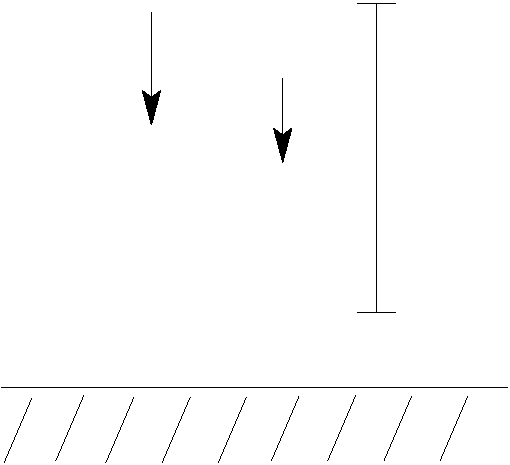
\includegraphics[height=12.7ex]{erde}}
		\put(11.0,17.2){\makebox(0,0)[l]{$A$}}
		\put(11.0, 8.5){\makebox(0,0)[l]{$B$}}
		\put( 7.8,16.0){\makebox(0,0){$m$}}
		\put( 3.5,15.0){\makebox(0,0)[r]{$g$}}
		\put(10.5,12.5){\makebox(0,0)[l]{$h$}}
		\put( 7.1, 4.0){\makebox(0,0)[t]{Earth}}
	\end{picture}
	%} %fbox
	\end{footnotesize}
	\caption{\label{fig:rotverschiebung}
		(a) Redshift by acceleration.
		(b) Redshift by gravitation.
	}
\end{figure}
%--- figure ----------------------------------------------------------
At time $t=0$, the lower observer sends a photon $\gamma$ in the direction of
the upper observer. Let us assume that the spacecraft is at rest at time $t=0$
relative to an initial system. Let $v=gt$ be the velocity of the two
observers after time $t$. Under the assumption $v \ll c$, we can
neglect terms of the order $v/c$ in the following approximation.
Then the photon reaches the upper observer in the time $t \approx h/c$.
Now the upper observer has reached the velocity $v = gt \approx gh/c$.
Due to the Doppler effect, he observes the photon with a redshift
\begin{equation}
	z := \frac{\Delta \lambda}{\lambda}
	\approx \frac{v}{c} \approx \frac{gh}{c^2}.
	\label{eq:rotverschiebung-1}
\end{equation}
According to the equivalence principle, the same redshift can also be expected for two observers
in a homogeneous gravitational field.
Since for a weak homogeneous gravitational field (such as on the Earth's surface)
$\Delta \Phi = gh$
applies to Newton's gravitational potential $\Phi$, we can also write Newton's approximation for the redshift
\begin{equation}
	z = \frac{\Delta \Phi}{c^2}
	.
	\label{eq:rotverschiebung-2}
\end{equation}
This formula could be confirmed up to 1\% by terrestrial experiments basing on the Möß\-bauer effect\index{Mößbauer effect}.

The redshift (\ref{eq:rotverschiebung-1}), however, also follows from the conservation of energy. Let us assume two points $A$ and $B$ in a homogeneous
gravitational field $g$ at a distance $h$ (Figure \ref{fig:rotverschiebung}b).
A mass $m$ falls from $A$ to $B$ with an initial velocity of 0.
At point $B$, according to Newton's theory, it has a kinetic energy
$E_{\mathrm{kin}} = mgh$. Now let us imagine that the entire energy
of the falling body, i.e., rest energy plus kinetic energy, is annihilated at point $B$
into a photon that moves back to point $A$ in the gravitational field.
If the photon had no interaction with the gravitational field, If the photon did not interact with the gravitational field,
we could convert it back into a mass $m$ there and would gain the energy $\Delta E = mgh$ in
this circular process.
In order to preserve the law of conservation of energy, the photon must therefore be shifted to the red. Therefore we obtain the following identities for the photon energy
$$
	E_{\mathrm{below}}
	= E_{\mathrm{above}} + mgh
	= mc^2 + mgh
	= mc^2 \left( 1 + \frac{gh}{c^2}\right)
	= E_{\mathrm{above}} \left( 1 + \frac{gh}{c^2}\right)
	.
$$
This means the the change of wave length
\begin{equation}
	1+z 
	= \frac{\lambda_{\mathrm{above}}}{\lambda_{\mathrm{below}}}
	= \frac{\hbar \omega_{\mathrm{below}}}{\hbar \omega_{\mathrm{above}}}
	= \frac{E_{\mathrm{below}}}{E_{\mathrm{above}}}
	= 1 + \frac{gh}{c^2}
	,
\end{equation}
coincides with (\ref{eq:rotverschiebung-1}).


\section{Exact vacuum solutions of the field equations}

Historically, the first exact solutions of the Einstein field equations with vanishing cosmological constant were found by Karl Schwarzschild in 1916 and by Alexander Friedmann in 1922. Schwarzschild's solution describes the gravitational field in a vacuum, enabling eventually the representation black holes, whereas Friedmann's solution represents a universe filled with a matter fluid of given density and pressure.
In this section we shortly consider the first one as a prominent vacuum solution. We return to Friedmann's solution below in chapter \ref{sec:FLRW-universes}.


%\subsection{Vacuum solutions}

The simplest class of exact solutions to Einstein's
field equations (\ref{eq:Feldgleichungen}), with $\Lambda = 0$, are the
\emph{vacuum solutions}\index{vacuum solutions}.
They solve the field equations with a vanishing
energy-momentum tensor, i.e.,
\begin{equation}
	T_{ij}
	= \left(\begin{array}{cccc}
		0   &   0   &   0   &  0 \\
		0   &   0   &   0   &  0 \\
		0   &   0   &   0   &  0 \\
		0   &   0   &   0   &  0
	\end{array}\right)
	.
	\label{eq:T-ij=0}
\end{equation}
The vacuum solutions thus represent gravitational fields in
a vacuum.
Since the field equations with (\ref{eq:T-ij=0}) are relatively
easy to solve, the first exact solutions to be discovered were two vacuum solutions:
the Minkowski space-time (by construction according to the equivalence principle, of course) and the Schwarzschild solution.


\subsection{Minkowski spacetime of special relativity}
The simplest solution to the field equation is the
\emph{Minkowski spacetime}\index{Minkowski spacetime}.
Its metric tensor in orthogonal coordinates $(t, x, y, z)$ is constant
\begin{equation}
	g_{ij}
	= \left(\begin{array}{@{}rrr@{\hspace*{3.5ex}}c}
		1   &   0   &    0   &  0 \\
		0   &  -1   &    0   &  0 \\
		0   &   0   &   -1   &  0 \\
		0   &   0   &    0   & -1
	\end{array}\right)
	.
	\label{eq:g-Minkoski}
\end{equation}
Since all derivatives of $g_{ij}$ disappear, space
and time are not curved.
In particular, light rays move in straight lines here,
but there is also no gravity.
Min\-kow\-ski space-time is the model of special
relativity.
Of course, Einstein knew this trivial solution
to his field equations; he had deliberately constructed his system of equations
in such a way that Minkowski spacetime would solve them,
cf. the correspondence principle above. However, for a non-vanishing cosmological constant this principle is not satisfied. \cite[151]{Straumann-1988}


\subsection{Black holes}
Einstein himself was unable to determine a non-trivial exact solution to his field equations.
But only a few months after their
publication, the astronomer Karl Schwarzschild succeeded in
finding the first exact solution to the complicated differential equations
for the case of a vacuum outside a given mass.
%It belongs to the class of \emph{vacuum solutions}\index{vacuum solution},
%It belongs to the class of \emph{vacuum solutions}\index{vacuum solution},
%i.e., the field equations for a vanishing energy-momentum tensor,
%\begin{equation}
%    T_{ij} = 0.
%\end{equation}
The solution found by Schwarzschild and now named after him
ultimately describes a black hole\index{black hole},
but this was not understood as a possible physical reality
until the 1960s. The metric tensor that solves the field equations has a
simple diagonal form
\begin{equation}
	g_{ij}
	= \left(\begin{array}{cccc}
		g_{tt} &   0    &   0    &  0     \\
		   0   & g_{rr} &   0    &   0    \\
		   0   &   0    & g_{\vartheta\vartheta} &  0 \\
		   0   &   0    &   0    & g_{\varphi\varphi} \\
	\end{array}\right)
	\label{eq:Schwarzschild-schema}
\end{equation}
and is usually described by the coordinates $(r, \vartheta, \varphi, ct)$,
where $t$ is time and 
$(r, \vartheta, \varphi)$
are the spatial spherical coordinates.
The  three spatial components of $g_{ij}$ have
a sign different from $g_{tt}$,
and the magnitude of the $g_{rr}$ component
is the reciprocal of the magnitude of $g_{tt}$,
\begin{equation}
	g_{rr} = -\frac{1}{g_{tt}}
    .
\end{equation}
In the 1960s, Kerr discovered an exact solution that generalized the Schwarzschild solution and contains non-vanishing
components in the secondary diagonal.
The Kerr solution represents a rotating gravitational source
in a vacuum. \cite[Chap. 6]{Chandrasekhar-1983} %\cite{de-Vries-2009}


%\subsection{Non-vacuum solutions: Models of the universe}
%
%The energy-momentum tensor 
%\begin{equation}
%	T_{ij}
%	= \left(\begin{array}{@{}rccc}
%	  \rho  &  0   &   0   &  0 \\
%		0   &  -p  &   0   &  0 \\
%		0   &  0   &  -p   &  0 \\
%		0   &  0   &   0   & -p \\
%	\end{array}\right)
%\end{equation}
%with two positive differentiable functions 
%$p = p(t)$ und $\rho = \rho(t)$
%represents physically an ideal fluid
%with pressure $p$ and energy density $\rho$.
%%As early as 1914, Einstein had described it as an example of a
%%non-vanishing energy-momentum tensor.
%With the “chronometric coordinates”
%$(\chi,\theta,\varphi, \tau)$, where 
%$(\chi,\theta,\varphi)$
%are spatial polar coordinates for $k \leqq 0$, similar to the Schwarzschild solution,
%and four-dimensional spherical coordinates for $k=1$
%\cite[§111]{Landau-Lifschitz-1997},
%as well as the differentiable functions $a = a(\tau)$ and
%\begin{equation}
%	f_k(\chi) = \left\{\begin{array}{@{\ }ll}
%        \sinh \chi & \mbox{for $k=-1$,} \\
%        \chi       & \mbox{for $k=0$,} \\
%        \sin \chi  & \mbox{for $k=1$.}
%    \end{array}\right.
%	\label{(3.23)}
%\end{equation}
%%In this section, we often write $f$ instead of $f_k$.
%we can then solve the field equations with the metric tensor
%\begin{equation}
%    g_{ij}
%	= a^2 \left(\begin{array}{@{\,}rccc}
%        1  &    0   &   0    &  0     \\
%        0  &   -1   &   0    &  0     \\
%        0  &    0   & -f_k^2 &  0     \\
%		0  &    0   &   0    & -f_k^2 \sin^2 \vartheta \\
%    \end{array}\right)
%    \label{eq:Robertson-Walker-Metrik}
%\end{equation}
%For more details, see, for example, \cite[§3.2]{de-Vries-1994}.
%%
%With the change of coordinates 
%%$(0, \infty) \times \tilde I_k \to (0, \infty) \times J_k$,
%$(\tau, \chi) \mapsto (t,r)$,
%\begin{equation}
%	\tau \mapsto t = \sigma(\tau), \qquad \chi \mapsto r = f_k(\chi),
%	\label{eq:Koordinatenwechsel}
%\end{equation}
%i.e., with
%\begin{equation}
%	\tau = \sigma^{-1}(t), \qquad
%	\chi = f_k^{-1}(r) = \left\{\begin{array}{@{\ }ll}
%		\mathrm{arsinh}\, r & \mbox{für $k=-1$,} \\
%		r & \mbox{für $k=0$,} \\
%		\arcsin\, r & \mbox{für $k=1$,}
%	\end{array}\right.
%	\label{(3.30)}
%\end{equation}
%and with the \emph{world radius}\index{world radius}
%\begin{equation}
%	R(t) := a\big(\sigma^{-1}(t)\big)\, /\, c,
%	\label{eq:def-R}
%\end{equation}
%$c$ the speed of light, we have
%\begin{equation}
%	\D \tau = \frac{c \D t}{R(t)}, \quad \mbox{bzw.} \quad c \D t = a(\tau) \D \tau, \qquad
%	\D\chi = \frac{\D r}{\sqrt{1 - kr^2}}\,.
%	\label{(3.32)}
%\end{equation}
%Therefore the metric reads
%\begin{equation}
%	\D s^2 = c^2 \D t^2 - R^2(t) 
%	\left( \frac{\D r^2}{1 - kr^2} + r^2 \D \theta^2 + r^2 \sin^2 \theta \D \varphi^2 \right).
%	\label{eq:Robertson-Walker}
%\end{equation}
%This is the \emph{Friedmann-Lemaître-Robertson-Walker} (FLRW) line element, the metric of a spactime that is obtained from the \emph{cosmological princip}\index{cosmological principle} of spacelike isotropy. \cite{Sexl-Urbantke-1987}, \cite[§5.3]{Hawking-Ellis-1973}.
%The parameter $t$ is the \emph{cosmic time}\index{cosmic time}.
%
%If, according to (\ref{eq:Koordinatenwechsel}), we only perform the coordinate transformation $\tau \mapsto t$, 
%then the line element of the metric tensor
%(\ref{eq:Robertson-Walker-Metrik}) with (\ref{eq:def-R}) for $k=1$ is
%\[
%	\D s^2 = c^2 \D t^2 - R^2(t) 
%	\left(\D \chi^2 + \sin^2 \chi \D\theta^2 + \sin^2\chi\sin^2 \theta \D\varphi^2 \right).
%\]
%The spatial part 
%$R^2(t) \left(\D \chi^2 + \sin^2 \chi \D\theta^2 + \sin^2\chi\sin^2 \theta \D\varphi^2 \right)$ 
%thus is exactly the three-dimensional line element of a hypersphere with radius $R$ embedded in Euclidian $\mathbb{R}^4$. This explains the designation “worl radius” for $R$. \cite[pp. 149]{Sexl-Urbantke-1987}.
%
%A physical model of the universe is obtained by
%substituting (\ref{eq:Robertson-Walker}) into Einstein's field equations with the energy-momentum tensor
%of an ideal fluid (“galactic gas”). This ultimately yields an
%ordinary nonlinear differential equation for $R(t)$, the \emph{Friedmann equation}
%\cite[pp.~156]{Sexl-Urbantke-1987}.
%%If $R(t)$ is a solution to this equation, the associated Robertson-Walker spacetime is called the \emph{Friedmann cosmos}.
%
% For  the  special  case  of  a  vanishing  cosmological constant
%(“vacuum energy density”), the Friedmann equation for a 
%matter-dominated  universe  (“incoherent”  or  “dust-like  matter”) reduces to the
%simple equation $(\D R/\D t)^2 = \mathscr{A}/R - k$, $\mathscr{A}$ $=$ const, which takes the form
%\[
%	(\dot{a})^2 = A_0 a - k a^2
%\]
%with $A_0 = \mathscr{A}/c^2$. \cite[p.~237]{Stephani-1991} 
%Separation of variables yields the solutions
%\begin{equation}
%	a(\tau) = \left\{ \begin{array}{@{\ }ll}
%		\frac12\, A_0 (\cosh \tau - 1) & \mbox{für $k = -1$,} \\[1.0ex]
%		\frac14\, A_0 \tau^2 & \mbox{für $k = 0$,} \\[1.0ex]
%		\frac12\, A_0 (1 - \cos \tau) & \mbox{für $k = 1$}
%	\end{array}\right.
%	\label{(3.34)}
%\end{equation}
%%mit $\tau \in I_k$. 
%By (\ref{eq:Koordinatenwechsel}) we then have 
%%$t = \frac{1}{c} \int a \D \tau$, d.h.\ $t \in J_k$,
%\begin{equation}
%	t = \left\{ \begin{array}{@{\ }ll}
%		\frac{1}{2c}\ A_0 (\sinh \tau - 1) & \mbox{für $k = -1$,} \\[1.0ex]
%		\frac{1}{12\,c}\ A_0 \tau^3 & \mbox{für $k = 0$,} \\[1.0ex]
%		\frac{1}{2c}\ A_0 (1 - \sin \tau) & \mbox{für $k = 1$.}
%	\end{array}\right.
%\end{equation}
%Since $a$ (except for a positive factor corresponding to the radius of the universe) describes the expansion of the universe,
%there are three different development scenarios depending on the parameter $k$, Fig. \ref{fig:Friedmann-Kosmen}.
%The first scenario $k = +1$ is the so-called “big crunch,” in which the universe collapses into a singularity after reaching its maximum expansion. This scenario is based on the assumption that the universe is finite and has a finite volume.
%\begin{figure}[htp]
%\centering
%\begin{footnotesize}
%\begin{tikzpicture}[>=stealth, domain=0:3.5, scale=0.4]
%	\draw[->] (-0.2,0) -- (11,0) node[right] {$t$};
%	\draw[->] (0,-.2) -- (0,7) node[left] {$a(t)$};
%	\draw[color=blue,thick]
%	plot ({sinh(0.9*\x) - 0.9*\x},{cosh(0.8*\x) - 1}) node[right] {$k = -1$};
%	\draw[color=gruen,thick]
%	plot ({.23*\x*\x*\x},{.45*\x*\x}) node[right] {$k = 0$};
%	\draw[color=rot,thick]
%	plot ({(3*\x - sin(150*\x))},{(1 - cos(150*\x))}) node[right] {$k = +1$};
%\end{tikzpicture}
%\hspace*{5ex}
%\begin{tabular}[b]{c}
%\begin{tikzpicture}[>=stealth, domain=0:3.5, scale=0.4]
%	\draw[->] (-2.0,0) -- (11,0) node[right] {$t$};
%	\draw[->] (0,-.2) -- (0,7) node[left] {$R(t)$};
%	\draw[color=gruen,thick]
%	plot ({.23*\x*\x*\x},{.55*\x*\x}) node[below] {$R(t)$};
%	\draw (-2,-.2) -- (9,7) node[left] {$h(t)$};
%	%\draw[circle (1ex)];
%	\draw[dashed] (3,-.2) -- (3,3); % node[left] {$R(t)$};
%	%\draw[dashed] (-1.7,-.2) -- (-1.7,3); % node[left] {$R(t)$};
%	\draw (3,0) node[below] {$t_0$}; % node[left] {$R(t)$};
%	\draw[|<->|,thick] (-1.7,3.5) --  node[above] {$\displaystyle \quad \frac{1}{H_0}$} (3,3.5);
%\end{tikzpicture}
%\\[-2.5ex]
%\end{tabular}
%\end{footnotesize}
%\caption{\label{fig:Friedmann-Kosmen}
%	Expansions of the three Friedmann cosmologies. The reciprocal of the Hubble constant $H_0$ represents an upper limit for the age of the universe, as can be seen from the tangent equation $h(t) = \dot{R}(t_0) (t-t_0) + R(t_0)$.}
%\end{figure}
%
%\noindent
%Also for a radiation-dominated Friedmann universe
%elementary solutions can be obtained for $\Lambda = 0$,
%cf. \cite[§26]{Stephani-1991}, 
%\cite[§5, especially pp. 156f and pp. 160ff]{Sexl-Urbantke-1987},
%\cite[p.~347ff]{O-Neill-1983},
%\cite[§§111--113]{Landau-Lifschitz-1997}.
%
%If we form the quotient of the derivative $\dot{R}$ of the world radius 
%and $R$, we obtain the relative rate of change of the universe
%\begin {equation}
%    H(t) = \frac{\dot{R}(t)}{R(t)}
%    ,
%\end{equation}
%the \emph{Hubble function} $H$.
%For the time $t_0$ $=$ now, $H_0$ $:=$ $H(t_0)$ 
%\emph{Hubble constant}\index{Hubble constant}.
%
%Its reciprocal $1/H_0$ indicates the maximum 
%age of the universe\index{age of the universe} for a non-accelerating
%expanding universe
%\cite{Sexl-Urbantke-1987}, because the equation of the tangent
%of the graph of $R(t)$ at the point $t_0$ is
%$h(t)$ $=$ $\dot{R}(t_0) (t-t_0) + R(t_0)$, 
%and its zero point is given by
%\begin{equation}
%	t_0 - t = \frac{R(t_0)} {\dot{R}(t_0)} = \frac{1}{H_0}
%\end{equation}
%given by \begin{equation}
%t_0 - t = \frac{R(t_0)} {\dot{R}(t_0)} = \frac{1}{H_0}
%\end{equation}
%see Figure \ref{fig:Friedmann-Kosmen}.
%
%Friedmann's models of the universe and more modern
%modifications such as the “inflationary universe” in its
%initial phase have repeatedly been confirmed by 
%physical observations. The first important
%confirmation was the discovery of the expansion of the universe
%
%Friedmann's models of the universe and more modern
%modifications such as the “inflationary universe” in its
%initial phase have repeatedly been confirmed by 
%physical observations. The first important
%confirmation was the discovery of the expansion of the universe
%by the Belgian priest and astrophysicist Georges Lemaître
%in 1927 \cite{Lemaitre-1927} and the US astronomer
%Edwin Hubble in 1929 \cite{Hubble-1929}.
%Further confirming observations were
%the discovery of cosmic background radiation by
%Penzias and Wilson in 1965 and the discovery of the Higgs boson
%in 2012, cf.
%\cite[§20.1]{Karttunen-et-al-2000},
%\cite[§13.3]{Unsoeld-Baschek-1999}


\section{General relativity in everyday life}
Most of the most important applications of general relativity are, naturally, in astronomy, especially
astrophysics and cosmology. After all, 
considerable gravitational fields or space and time scales are required to observe or utilize relativistic effects.
In everyday life, one would not expect Einstein's
hundred-year-old field equations to have any impact or even
significance at all.
After all, it is not exactly common to have a black hole in one's
handbag or a small inflationary universe in one's
closet.
And warp drive, which would allow one to travel to the nearest wormhole around the corner, is not yet functional.
It is therefore all the more surprising that there are indeed very practical
This makes it all the more astonishing that there are indeed very practical
applications and explanations of the general theory of relativity that 
affect our everyday lives.


\subsection{Olbers' paradox}
%\section{Der Himmel ist dunkel}
For a long time, it was an unexplained phenomenon that the sky is dark at night.
Olbers' paradox\index{Olbers' paradox} 
states the following:

\begin{satz}[\textbf{Olbers' paradox (1823) \cite{Olbers-1826}}]
	If the universe is infinite and uniform in space and time
    and filled with stars like our sun, 
    then the sky is at least
    as bright as the average luminosity $L$ of the stars everywhere.
	%\cite[§13.2.6]{Unsoeld-Baschek-1999}
\end{satz}
\begin{proof}
	\cite{Tipler-1988}
	Each spherical shell with radius $r$ and thickness $\D r$ around the Earth
    contains $4 \pi \rho r^2 \D r$ stars, where $\rho$ denotes the average star density.
    The apparent luminosity of a star on Earth is
    $L/r^2$.
	Therefore, each spherical shell 
    radiates with an apparent luminosity of $4 \pi \rho L \D r$.
    This integrand is constant and, in particular, independent of $r$.
%    The stars closer to Earth can absorb light sources behind them,
%    but due to the conservation of energy,
%    they must ultimately re-emit this energy.
\end{proof}

%\noindent
But why is it dark at night?
At least one of the three premises of the sentence must be false
so that it does not contradict our observations.
Either the universe is finite in space or time 
(or both),
or it is not uniformly filled with sun-like stars.
Einstein's field equations provide, for the first time in the
history of science, physically testable %quantifiable 
cosmological models
that solve Olbers' paradox by allowing for a temporally finite
universe.


\subsection{GPS}
GPS (Global Positioning System, officially NAVSTAR GPS) is a global satellite-based navigation system for determining position. To do this, the satellites constantly transmit their current position and the exact time using coded radio signals. GPS receivers can then calculate their own position and speed from the signal transit times. In theory, signals from three satellites with simultaneous radio contact are sufficient for this. 
%--- Figure: -----------------------------------------------------------
\begin{figure}[htp]
\centering
	\includegraphics[height=30ex]{GPS}
	\caption{\label{fig:GPS}
		Satellite-based navigation systems such as GPS
		(Source:
		\url{https://tug.org/TUGboat/tb33-1/tb103wolcott.pdf})
	}
\end{figure}
%--- Figure ------------------------------------------------------------
However, since GPS receivers do not necessarily use an accurate clock to measure the transit time, the signal from a fourth satellite is required to determine the exact time in the receiver.
GPS was launched in February 1978 and is based on 31 satellites.

A physical system rotating in a circular orbit around a static spherically symmetric 
gravitational field of mass $M$ can be described in general relativity by
the Schwarzschild metric \cite{de-Vries-1994,de-Vries-1996} 
with $\D r$ $=$ $\D \varphi$ $=$ $0$,
\begin{equation}
	\D s^2
	= c^2 \D \tau^2
	= \left(1 - \frac{2GM}{c^2 r}\right) c^2 \D t^2 - r^2 \D \vartheta^2
	.
\end{equation}
Here, $\tau$ denotes the proper time of the rotating system.
($t$ denotes the coordinate time of the entire gravitational field
and corresponds to the proper time of a stationary observer at infinity,
$r \to \infty$.)
It follows that
\begin{equation}
	\Big(\frac{\D \tau}{\D t}\Big)^2
	= \left(1 - \frac{2GM}{c^2 r}\right) 
	- \frac{r^2}{c^2} \, \frac{\D \vartheta}{\D t}
	= 1 + \frac{2 \Phi(r)}{c^2} - \frac{v^2}{c^2}
\end{equation}
with the gravitational potential $\Phi(r)$ 
%Relativitätstheorie $g_{44} = 1 - \Phi/c^2$
\cite[VI.2]{Straumann-1988}. %S. 261
and the orbital speed
$v(r)$ given by
\begin{equation}
	\Phi(r)
	= - \frac{M G}{r}
	, \qquad
	v(r) = r \, \frac{\D \vartheta}{\D t}
\end{equation}
This results in the proper times $\tau_E$ and $\tau_S$ of a receiver
on Earth with Earth radius $r_E$ and a satellite orbiting the Earth in a circular orbit
with radius $r_S$
\cite{Pascual-Sanchez-2007}
\begin{equation}
	\Big(\frac{\D \tau_S}{\D \tau_E} \Big)^2
	= \frac{1 + 2\Phi(r_S)/c^2 - v_S^2/c^2}
		{1 + 2\Phi(r_E)/c^2 - v_E^2 / c^2}
	\label{eq:GPS-Eigenzeiten}
\end{equation}
Since the gravitational field of the Earth is quite small on the Earth's surface,
 i.e., $\Phi(r_E)/c^2 \ll 1$, and since the velocities
$v_E$ and $V_S$ are much smaller than the speed of light,
the approximation
can be applied for equation (\ref{eq:GPS-Eigenzeiten}),
neglecting terms higher than $O(c^{-2})$, \cite{Pascual-Sanchez-2007,Singer-1956}.
\begin{equation}
	\frac{\D \tau_S}{\D \tau_E}
	= \frac{\sqrt{1 + 2\Phi(r_S)/c^2 - v_S^2/c^2}}
		{\sqrt{1 + 2\Phi(r_E)/c^2 - v_E^2 / c^2}}
	= %\approx
	1 + \frac{MG}{c^2} \left(\frac{1}{r_E} - \frac{1}{r_S}\right)
	+ \frac{v_E^2 - v_S^2}{2\, c^2}
	+ O(c^{-3})
	\label{eq:GPS-Zeitdilatation-approx}
\end{equation}
With the difference $\Delta \Phi = \Phi(r_E) - \Phi(r_S)$
between the two gravitational potentials and the difference
$\Delta v^2$ between the squares of the velocities,
\begin{equation}
	\Delta \Phi
	= {M G}
	\left(\frac{1}{r_E} - \frac{1}{r_S}\right)
	,
	\qquad
	\Delta v^2 = v_S^2 - v_E^2
	\label{eq:GPS-Potentialdifferenz}
\end{equation}
we thus have
\begin{equation}
	\frac{\D \tau_S}{\D \tau_E}
	\approx
	1 + \frac{\Delta \Phi}{c^2} - \frac{\Delta v^2}{2\,c^2}
	.
	\label{eq:GPS-Zeitdilatation}
\end{equation}
See \cite[Gl. (14.12)]{Sonne-Weiss-2013}.
This means that the time displayed by the atomic clocks on the GPS satellites is subject to special relativistic \emph{and} gravitational time dilation. According to general relativity, the rate at which a clock runs depends on its location in the gravitational field,
i.e., on $\Delta \Phi$, 
and according to special relativity, it depends on its velocity $v_S$.
The lower gravitational potential in the satellite's orbit causes time to pass more quickly than on Earth, while the orbital motion of the satellites relative to a stationary observer on Earth slows it down.
The two time dilations therefore have opposite effects.
In other words, for an observer on the Earth's surface, 
time passes 
slower than for an observer on the satellite, who is not moving relative to him, 
by a factor of $1 + \frac{\Delta \Phi}{c^2}$.

For the values
$M = 5.98 × 10^{24}$ kg, 
$r_E = 6.38 × 10^{6}$ m
and $r_S = 26.56 × 10^{6}$ m,
 equation (\ref{eq:GPS-Potentialdifferenz}) yields
$\Delta \Phi/c^2 = 5.28 \cdot 10^{-10}$
and
$\Delta v^2 = 8.5 \cdot 10^{-11}$ m/s.
In the GPS satellite orbit, the gravitational effect therefore predominates 
by more than six times: time therefore passes faster on the satellites. 
Equation (\ref{eq:GPS-Zeitdilatation}) yields
the relative satellite velocity $v_S = 3900$ m/s
and the relative rate difference  
\begin{equation}
	\frac{\D \tau_S}{\D \tau_E}
	= 1 + 4{,}44 \cdot 10^{-10}
\end{equation}
the proper times on Earth and in the satellite.
This ratio is significantly greater than the relative accuracy of cesium atomic clocks, which is of the order of $10^{-13}$.
To compensate for this time dilation, the oscillation frequency
of the satellite clocks is detuned to $\mu_{S}$ $=$ 10.229999995453 MHz, 
so that they always run synchronously with the frequency $\mu_{E}$ $=$ 10.23 MHz
of the terrestrial receiver clocks.
(The sample actually yields $\mu_E/\mu_S - 1 = 4.44 \cdot 10^{-10}$.)

If time dilation were not compensated for, the
difference in the rate of the clocks per year would add up to a time difference
of % between satellite clocks and clocks on Earth 
of approximately 0{,}014 seconds.
Accordingly, time dilation would lead to a deviation
\begin{equation}
	\frac{\D s}{\D \tau_E} - c
	= c \left(\frac{\D \tau_S}{\D \tau_E} - 1\right)
	= 0{,}133 \mbox{ m$/$s}
\end{equation}
Per second, the car would deviate 13 cm from its calculated
course, or 8 meters per minute or 11.5 km per day.
However, this error would not occur even without the corrective adjustment
of the satellite clocks in the real GPS system, because
at least four satellites are always contacted to determine time and location, so that only the satellite time is actually used.

%
At an altitude of about 3,000 km, 
special relativistic and gravitational time dilation
cancel each other out.

\chapter{Cosmological models}

In this chapter we will shortly review the standard models of cosmology. In essence they follow from the classes of geometry that are determined by the cosmological principle. In turn, the geometry and its symmetries prescribe the physical form and distribution of matter and energy in the universe, due to the Einstein field equations (\ref{eq:Feldgleichungen}).

The standard models of cosmology are essentially the three geometries of the Friedmann-Lemaître-Robertson-Walker metrics, each of which has variants with or without a cosmological constant, i.e., $\Lambda \ne 0$ or $\Lambda = 0$, respectively. The all rely on the cosmological principle, which in essence fixes the possible geometries and therefore prescribe the overall distribution of energy and matter in the cosmos.

The standard models of the universe all go back to Alexander Friedmann. They and more modern modifications such as the “inflationary universe” in its initial phase have repeatedly been confirmed by physical observations. The first important confirmation was the discovery of the expansion of the universe by the Belgian priest and astrophysicist Georges Lemaître in 1927 \cite{Lemaitre-1927} and the US astronomer Edwin Hubble in 1929 \cite{Hubble-1929}. Further confirming observations were the discovery of cosmic background radiation by Penzias and Wilson in 1965 and the discovery of the Higgs boson in 2012, cf.
\cite[§20.1]{Karttunen-et-al-2000},
\cite[§13.3]{Unsoeld-Baschek-1999}


\section{The cosmological principle}
The cosmological principle summarizes two basic assumptions of cosmology that underlie its models of the universe as a whole. %It has been introduced in 1933 by astrophysicist Edward A. Milne and states the following.

\begin{axiom}[\textbf{Cosmological principle}]
	\label{axiom:cosmological-principle}
	Viewed on a sufficiently large scale, the properties of the universe are the same for all observers.
	Especially the universe is homogeneous and isotropic.
	Homogeneity means that the universe appears the same to all observers regardless to their locations in space, isotropy means that the universe always appears the same to observers regardless of their direction of observation in space.
\end{axiom}

In general, the two concepts homogeneity and isotropy are independent. For instance, a structure of equidistant parallel lines is homogeneous in the plane, but not isotropic, and concentric lines are istropic around the center but not homogeneous. 

\begin{bem}
\label{bem:isotropy-and-constant-curvature}
From the point of view of differential geometry, isotropy at each point means local rotational symmetry everywhere and implies the space to have a constant curvature. Therefore, isotropy at each point implies homogeneity, but a homogeneous universe could be anisotropic somewhere.
\cite[448]{Karttunen-et-al-2000}, \cite[130]{Sexl-Urbantke-1987}
\end{bem}

The cosmological principle is based on the assumption that the uniformity of the universe observed from Earth cannot be explained by a special position, but rather by any position in the universe. This assumption cannot be proved. Its validity has to be assumed \emph{a priori}, i.e., it is an axiom.

The cosmological principle does not apply to small distances. For example, the density of matter in the solar system is significantly greater than in interstellar space. Furthermore, individual galaxies are not evenly distributed, but form groups, clusters, superclusters, and filaments. On an even larger scale, however, the cosmological principle has been repeatedly confirmed by increasingly accurate measurements.
%All of humanity's observations in all directions in space at distances of at least 100 million light-years, based on centuries of repeated measurements at various points in the Earth's orbit and a large number of satellites, space probes, and manned and unmanned space missions, confirm this assumption to date. This suggests that there is no systematic change in the density of matter in space and that the universe is infinite.


\section{Friedmann-Lemaître-Robertson-Walker universes}
\label{sec:FLRW-universes}

Translated into the language of Riemannian geometry, the cosmological principle implies that the three-dimensional space has maximum symmetry, i.e., has constant curvature which, if variable at all, can only depend on time. There are three possible geometries of space satisfying this criterion, depending on a parameter $k$. \cite[222]{Stephani-1991}
It will turn out that $k$ geometrically determines the spatial curvature of the universe, and physically $-k$ represents a part of its energy density. \cite[155]{Sexl-Urbantke-1987}

\begin{bem}
	One remarkable property of standard FLRW cosmology, as it will be described in the sequel, is that  the energy density of the universe depends on its \emph{global} geometry, represented by a discrete curvature parameter $k$. Of course, \emph{locally} this follows immediately from the Einstein field equations (\ref{eq:Feldgleichungen}), since geometry determines physics, and physics determines geometry. But \emph{globally} it is not clear at first sight, why there should be only three cases. In fact, this is a consequence of the strong symmetry requirements due to the cosmological principle \ref{axiom:cosmological-principle} and Remark \ref{bem:isotropy-and-constant-curvature}.
\end{bem}
%
For $k$ $\in$ \{$-1$, 0, 1\} let $\mathscr{M}_k$ denote one of the three manifolds
\begin{equation}
	\mathscr{M}_k = \left\{\begin{array}{cl}
		\mathbb{R}^4 & \mbox{for $k$ $=$ $-1$, 0,} \\
		\mathbb{R} \times S^3 & \mbox{for $k$ $=$ 1.}
	\end{array}\right.
	\label{eq:FLRW-manifolds} %{(3.20)}
\end{equation}
Define then the coordinates $(t,\chi,\theta,\varphi)$ $\in$ $\mathbb{R} \times I_k \times (0,\pi) \times (0, 2\pi)$ of $\mathscr{M}_k$ with the intervals
\begin{equation}
	I_k = \left\{ \begin{array}{ll}
		(0, \infty) & \mbox{for $k$ $=$ $-1$, 0,} \\
		(0, \pi) & \mbox{for $k$ $=$ 1,}
	\end{array}\right.
%	\qquad
%	J_k = \left\{ \begin{array}{@{\ }ll}
%		(0, \infty) & \mbox{for $k$ $=$ $-1$, 0,} \\
%		(-1, 1) & \mbox{for $k$ $=$ 1,}
%	\end{array}\right.
	\label{eq:FLRW-tau-interval} %{(3.21)}
\end{equation}
Especially for $k$ $=$ $-1$, $0$, let
$(\chi,\theta,\varphi)$ $\in$ $(0, \infty) \times (0,\pi) \times (0, 2\pi)$
denote the polar coordinates of $\mathbb{R}^3$ (with the radial coordinate $\chi$). For $k$ $=$ $1$, on the other hand, let $(\chi, \theta, \varphi)$ $\in$ $(0, \pi) \times (0,\pi) \times (0, 2\pi)$ denote the polar coordinates of $S^3$ (i.e., $\chi$ is an angular coordinate). Moreover, let
\begin{equation}
	R \in C^\infty(\mathbb{R}, (0, \infty)), \qquad t \mapsto R(t),
	\label{eq:FLRW-R} %{eq:FLRW-a} %{(3.22)}
\end{equation}
be a function depending on $t$, and let $f_k$: $I_k \to J_k$ denote the functions
\begin{equation}
	f_k(\chi) = \left\{\begin{array}{@{\ }ll}
		\sinh \chi & \mbox{for $k=-1$,} \\
		\chi       & \mbox{for $k=0$,} \\
		\sin \chi  & \mbox{for $k=1$.}
	\end{array}\right.
	\label{(3.23)}
\end{equation}
%We often simply write $f$ instead of $f_k$.
The parameter $t$ is called \emph{cosmic time}\index{cosmic time},
and $R$ the \emph{scale factor} of the universe. 
Defining the covariant %and contravariant 
components of the metric tensor by
\begin{eqnarray*}
	(g_{ij}) & \hspace*{-1.5ex} = \hspace{-1.5ex} & 
	\mathrm{diag}\,(1, -R^2, -R^2 f_k^2, - R^2 f_k^2 \sin^2\theta)
%	\\
%	(g^{ij}) & \hspace*{-1.5ex} = \hspace{-1.5ex} & 
%	\frac{1}{a^2}\ \mathrm{diag} \left(1, -1, -\frac{1}{f_k^2}- \frac{1}{f_k^2 \sin^2\theta}\right)
	,
\end{eqnarray*}
the line element reads
\begin{equation}
	\D s^2 = 
	\D t^2 - R^2(t) \left( \D\chi^2 - f_k^2(\chi) \D \theta^2 - f_k^2(\chi) \D\varphi^2 \right)
	.
	\label{eq:FLRW-line-element-in-polar-coordinates} %{(3.26)}
\end{equation}
cf. \cite[(112,2)]{Landau-Lifschitz-1997}. 
%We have
$ %\begin{equation}
	\sqrt{g} = R^3(t) \, f_k^2(\chi) \sin \theta.
%	\label{(3.27)}
$ %\end{equation}
For $k=1$, the spatial part of(\ref{eq:FLRW-line-element-in-polar-coordinates}), i.e.,
$R^2(t)\, (\!\D \chi^2 + \sin^2 \chi \D\theta^2 + \sin^2\chi\sin^2 \theta \D\varphi^2 )$, 
is exactly the three-dimensional line element of a hypersphere with radius $R(t)$ embedded in Euclidian space $\mathbb{R}^4$. Therefore, the scale factor $R$ is sometimes also called the \emph{world radius}\index{world radius}.
\cite[pp.~149]{Sexl-Urbantke-1987}
Especially, for $k=1$ the universe has a finite volume. In general, the volume of a 3-space with coordinates $(x_1, x_2, x_3)$ and a metric with determinant $g$ is defined as $V$ $=$ $\iiint \! \sqrt{g} \D x_1\D x_2 \D x_3$, cf. (\ref{eq:volume-element}). For the line element (\ref{eq:FLRW-line-element-in-polar-coordinates}) we therefore have
\begin{align}
	V 
	& = 
	\int\limits_0^\pi \! \int\limits_0^\pi \! \int\limits_0^{2\pi} \! \sqrt{g} \D \varphi \D \theta \D r
	=
	R^3(t)  \int\limits_0^\pi \! \sin^2 \chi  \D \chi \cdot \int\limits_0^\pi \! \sin \theta   \D \theta \cdot \int\limits_0^{2\pi} \! \D \varphi
%	\nonumber \\ & =
%	R^3(t) \cdot \frac{1}{2} \, (\chi - \sin \chi \cos \chi)\, \Big|_0^\pi 
%	\cdot (- \cos \theta) \, \Big|_0^\pi \cdot \varphi \, \Big|_0^{2\pi}
%	=
%	R^3(t) \cdot \frac{\pi}{2} \cdot 2 \cdot 2\pi
%	\nonumber \\ & 
	=
	2 \pi^2 R^3(t).
	\label{eq:FLRW-volume-k=1}
\end{align}

\begin{bem}
\label{Bemerkung 3.7}%
In cosmology it is more familiar to consider another coordinate than $\chi$, namely the parameter
$r \in J_k$, with $J_k = I_k$ for $k=0,-1$ and $J_1 = (0,1)$ for $k=1$, given by
\begin{equation}
	\chi \mapsto r = f_k(\chi),
	\label{eq:FLRW-r} % {eq:FLRW-coordinate-cosmic-time} %{(3.29)}
%\end{equation}
%i.e.,
	\qquad \mbox{i.e.,} \qquad
%\begin{equation}
	\D\chi = \frac{\D r}{\sqrt{1 - kr^2}}\,.
	%\label{(3.32)}
\end{equation}
where $	\chi = f_k^{-1}(r) \in (0, \frac{\pi}{2})$.
%\begin{equation}
%	\chi = f_k^{-1}(r) = \left\{\begin{array}{@{\ }ll}
%		\mathrm{arsinh}\, r & \mbox{for $k=-1$,} \\
%		r & \mbox{for $k=0$,} \\
%		\arcsin\, r & \mbox{for $k=1$,}
%	\end{array}\right.
%	\label{(3.30)}
%\end{equation}
Thus the metric (\ref{eq:FLRW-line-element-in-polar-coordinates}) transforms to
\begin{equation}
	\D s^2 = c^2 \D t^2 - R^2(t) 
	\left( \frac{\D r^2}{1 - kr^2} + r^2 \D \theta^2 + r^2 \sin^2 \theta \D \varphi^2 \right)
	,
	\label{eq:FLRW-line-element} %{(3.33)}
\end{equation}
and the determinant of the metric is $\sqrt{g} = R^3(t) \frac{r^2}{\sqrt{1 - r^2}}$.
This is the line element of the \emph{Fried\-mann-Lemaître-Robertson-Walker (FLRW) models}.
It is a metric of a space-time that is obtained from the {cosmological principle} of space-like isotropy at each fixed cosmic time $t = \mathrm{const}$. \cite{Hawking-Ellis-1973}, \cite{Sexl-Urbantke-1987}

For $k=1$, i.e., a three-dimensional hypersphere $S^3(R)$ with world radius $R$, the metric gets singular at $r=1$. However, this is not a physical singularity, but a pure coordinate singularity. An analogy in two dimensions may illustrate this, see Fig. \ref{fig:S2-coordinate-change-analogy-to-FLRW-metric}. 
%--- Figure: ---------------------------------------------------------
\begin{figure}[htp]
\centering
\includegraphics[scale=1]{S2-coordinate-change-analogy-to-FLRW-metric}
\caption[The FLRW cosmological models]{\label{fig:S2-coordinate-change-analogy-to-FLRW-metric}
	The coordinate change $(\chi, \varphi) \mapsto (r, \varphi)$ on the sphere $S^2(R)$ embedded in three-space $\mathbb{R}^3$, as an analog to the coordinate change (\ref{eq:FLRW-r}) on $S^3(R)$.
	Graphics modified from \cite[151]{Sexl-Urbantke-1987}
}	
\end{figure}
%--- Figure^ ---------------------------------------------------------
We have $r = \sin \chi$, but there is no singularity at the equator $\chi = \frac{\pi}{2}$.
Moreover, this analogy illustrates the role of the cosmological scale factor $R$.
A sphere $S^2$ is a two-dimensional surface embedded in a 3-dimensional space. Its radius lives in the third dimension, it is not part of the surface. However, the value of this radius affects distances measured on the two-dimensional surface. Similarly, the cosmological scale factor is not a distance in our 3-dimensional space, but its value affects the measurement of distances.
%
%%The coordinates $(\tau, \chi, \theta, \varphi)$ are also called  \emph{chronometrical comoving}.
%%%\cite{Villalba-Percoco-1991} or 
%%\cite{Landau-Lifschitz-1997}
%From the function $a$, or equivalently the world radius $R$, the \emph{Hubble constant} $H$ is defined by %\cite[445]{Landau-Lifschitz-1997}
%\[
%	H = c\ \frac{\dot{a}}{a^2} = \frac{1}{R(t)}\, \frac{\D R}{\D t}
%\]
%e.g., \cite[p.~445]{Landau-Lifschitz-1997}.
%% ---
%For 
%$\dot{a}>0$ the Friedmann-Lemaître-Robertson-Walker space-time describes an expanding universe, whereas for $\dot{a}<0$ it is a \emph{contracting} one.
\end{bem}


\section{Solving the field equations by FLRW geometries}

So far, we only derived the \emph{geometry} of a universe satisfying the cosmological principle. To solve the Einstein field equations (\ref{eq:Feldgleichungen}), however, we have to find suitable distributions of energy and matter in the spacetime, determined by $T_{ij}$. In other words, a physical model of the universe is derived, if (\ref{eq:FLRW-line-element}) is inserted in the Einstein field equations.
By the strong spatial symmetries implied by the cosmological principle they only can determine the evolution of the universe in time, i.e., its dynamics.
It turns out that, given the FLRW geometry, the energy-momentum tensor must represent an ideal fluid with pressure $p$ and energy density $\rho$, i.e., must be of the form 
\begin{equation}
	T_{ij}
	= 
	p g_{ij} + (\rho + p/c^2) u_i u_j
%	\left(\begin{array}{@{}cccc}
%	  c^2\rho  &  0  &  0  &  0 \\
%		0   &  p  &  0  &  0 \\
%		0   &  0  &  p  &  0 \\
%		0   &  0  &  0  &  p \\
%	\end{array}\right)
\end{equation}
with $c$ the speed of light and $u_i$ the four-velocity of the fluid with respect to the rest system of the FLRW metric (\ref{eq:FLRW-line-element}).
Moreover, $p$ and $\rho$ depend only on the cosmic time but not on their spatial positions, i.e., $p = p(t)$ and $\rho = \rho(t)$.
\cite[83,233-234]{Stephani-1991}
In the rest system of the fluid, we have
\begin{equation}
	T_{ij}
	=
	\left(\begin{array}{@{}cccc}
	  c^2\rho  &  0  &  0  &  0 \\
		0   &  p  &  0  &  0 \\
		0   &  0  &  p  &  0 \\
		0   &  0  &  0  &  p \\
	\end{array}\right)
\end{equation}
Inserting this tensor into the Einstein field equations yields the two ordinary differential equations for $R(t)$,
\begin{equation}
	%2 \ddot{R}/R + (\dot{R}^2 + k)/R^2 
	\frac{\dot{R}^2}{R^2} + \frac{2 \ddot{R}}{R} + \frac{c^2 k}{R^2} 
	= 
	- \kappa p + c^2 \Lambda
	\label{eq:FLRW-dynamics-1}
\end{equation}
and
\begin{equation}
	%3 \, (\dot{R}^2 + k)/R^2 = 
	\frac{3 \dot{R}^2}{R^2} + \frac{3 c^2 k}{R^2} = 
	\kappa c^4 \rho + c^2\Lambda
	\label{eq:FLRW-dynamics-2}
\end{equation} 
\cite[154]{Sexl-Urbantke-1987}, \cite[234]{Stephani-1991}
Here $\dot{R}$ denotes the derivative with respect to the cosmic time, i.e., $\dot{R} = \!\D R/\!\D t$.
For $p=0$, these equations have been derived first by Friedmann in 1922. \cite[(4) \& (5)]{Friedmann-1922}
%Rearranging (\ref{eq:FLRW-dynamics-2}) for $\frac{\dot{R}^2}{R^2}$ and inserting this in (\ref{eq:FLRW-dynamics-1}) gives
Subtracting $\frac{1}{6}$ times (\ref{eq:FLRW-dynamics-2}) from $\frac{1}{2}$ times (\ref{eq:FLRW-dynamics-1}) gives
\begin{equation}
	\frac{\ddot{R}}{R}
	= \frac{c^2\Lambda}{3}
	- \frac{\kappa c^4}{6} \left( \rho + 3p/c^2 \right)
	.
	\label{eq:FLRW-dynamics-1'}
\end{equation}
cf. \textcite[485]{Unsoeld-Baschek-2002}.
Hence the system of the two equations (\ref{eq:FLRW-dynamics-1}) and (\ref{eq:FLRW-dynamics-2}) is equivalent to the system of (\ref{eq:FLRW-dynamics-1'}) and (\ref{eq:FLRW-dynamics-2}). Nowadays, (\ref{eq:FLRW-dynamics-2}) and (\ref{eq:FLRW-dynamics-1'}) are called \emph{Friedmann equations}\index{Friedmann equations}.
Note that equation (\ref{eq:FLRW-dynamics-1'}) does not contain the geometric parameter $k$, in contrast to Friedmann's original equation (\ref{eq:FLRW-dynamics-1}).

Equation (\ref{eq:FLRW-dynamics-1'}) states that both the energy density and the pressure cause the expansion rate of the universe $\dot{R}$ to decrease. This is a consequence of gravitation, with pressure playing a similar role to that of energy density. The cosmological constant, on the other hand, causes an acceleration in the expansion of the universe.
Under the assumption that the total mass of the universe is constant, i.e., $\rho R = \mathrm{const}$, Equation (\ref{eq:FLRW-dynamics-1}) on the other hand expresses the energy conservation of the universe. \cite[155]{Sexl-Urbantke-1987}

Another important identity can be deduced from the Friedmann equations, assuming that all the terms $R$, $\dot{R}$, and $(c^2 \rho + p)$ do nat vanish: Deriving first (\ref{eq:FLRW-dynamics-2}) times $R^2$ with respect to $t$, rearranging the resulting equation for $\ddot{R}/R$, and inserting this into (\ref{eq:FLRW-dynamics-1'}), we obtain
\begin{equation}
	\frac{\dot{\rho}}{\rho + p/c^2} = - \frac{3 \dot{R}}{R}
	.
	\label{eq:FLRW-dynamics-3}
\end{equation}
cf. \cite[(26,9)]{Stephani-1991}.
Physically this equation expresses the first law of thermodynamics, assuming the expansion of the universe is an adiabatic process, i.e., a process without a change of entropy.


\section{FLRW models with $\fettgr{\Lambda}$ = 0 and \textit{p} = 0: Exact solutions}
\label{sec:FLRW-Lambda=0-p=0}
The Friedmann equation (\ref{eq:FLRW-dynamics-1'}) expresses the dynamics of the FLRW models. That is, the behavior in time follows from the energy density $\rho$ and the pressure $p$.
In a matter-dominated universe, as we observe it today, we have $p \approx 0  < \rho$. A cosmos like this is also called “incoherent” or “dust-like”.
If we set $p=0$ and let moreover the cosmological constant vanish, 
%the Friedmann equation (\ref{eq:FLRW-dynamics-2}) 
(\ref{eq:FLRW-dynamics-3})
reduces to $\dot{\rho}/\rho = - 3\dot{R}/R$ and can be immediately integrated by
\begin{equation}
	\rho R^3 = \mathscr{A} = \mathrm{const}
	.
	\label{eq:FLRW-Lambda=p=0-integration-constant}
\end{equation}
The integration constant $\mathscr{A}$ can be interpreted as a multiple of the total mass $\mathfrak{M}$ of the universe. With (\ref{eq:FLRW-volume-k=1}), for instance, we have $\mathfrak{M} = 2 \pi^2 \mathscr{A}$.
By (\ref{eq:FLRW-Lambda=p=0-integration-constant}) we have $\rho = \mathscr{A}/R^3$, i.e., equation (\ref{eq:FLRW-dynamics-2}) simplifies to
$(\dot{R})^2 = {\kappa c^2 \mathscr{A}}/{R} - k$, which by the transformation $t \mapsto \tau = \pm \frac{1}{c}\int \! \frac{\D t}{R(t)}$,
i.e., $\D \tau = \pm \frac{c}{R} \D t$ or $\frac{\DD}{\DD t} = \pm \frac{c}{R} \frac{\DD}{\DD \tau}$, 
attains the form
\begin{equation}
	(R')^2 = \kappa \mathscr{A} R / 3 - k R^2
	\label{eq:FLRW-dynamics-simple-case}
\end{equation}
with $A_0 = \kappa \mathscr{A}/3$, and $'$ denoting the derivative with respect to $\tau$. \cite[237]{Stephani-1991}
Separation of variables\footnote{
	In more detail, %with $A_0 = \kappa \mathfrak{M}/3$ 
	separation of variables (\ref{eq:FLRW-dynamics-simple-case})
	yields
	$
		\frac{\D R}{\sqrt{A_0 R - k R^2}} = \pm\!\D \tau
	$,
	or
	$\pm\tau = \int \frac{\D R}{\sqrt{A_0 R - k R^2}}$.
	For $k=-1$ this is 
	$\pm\tau 
	= \int \frac{\D R}{\sqrt{A_0 R + R^2}}
	= \mathrm{arcosh}\, (1 + 2R/A_0)
	$,
	for $k=0$ we have 
	$\pm\tau 
	= \int \frac{\D R}{\sqrt{A_0 R}}
	= 2 \sqrt{R/A_0}
	$,
	and for $k=1$, finally,
	$\pm\tau 
	= \int \frac{\D R}{\sqrt{A_0 R - R^2}}
	= \arccos (1 - 2R/A_0)
	$.
	The identities for the integral can be shown elementarily by derivation with respect to $R$.
	Rearranging the equations for $R$ yields (\ref{eq:FLRW-solutions-Lambda=0}), independently from the sign of $\tau$.
}
then yields the solutions
\begin{equation}
	R(\tau) = \left\{ \begin{array}{@{\ }ll}
		\frac{1}{2}\, A_0 \, (1 - \cos \tau) & \mbox{for $k = 1$,}
		\\[1.0ex]
		\frac{1}{4}\, A_0 \, \tau^2 & \mbox{for $k = 0$,}
		\\[1.0ex]
		\frac{1}{2}\, A_0 \, (\cosh \tau - 1) & \mbox{for $k = -1$,}
%		\frac{\kappa \mathfrak{M}}{6}\, (\cosh \tau - 1) & \mbox{for $k = -1$,} \\[1.0ex]
%		\frac{\kappa \mathfrak{M}}{12}\, \tau^2 & \mbox{for $k = 0$,} \\[1.0ex]
%		\frac{\kappa \mathfrak{M}}{6} (1 - \cos \tau) & \mbox{for $k = 1$}
	\end{array}\right.
	\label{eq:FLRW-solutions-Lambda=0} %{(3.34)}
\end{equation}
with $\tau \in I_k$. The cosmic time then satisfies $t = \frac{1}{c} \int_0^\tau R \D \tau$, 
i.e., $t \in J_k$ and
\[
	t = \pm \left\{ \begin{array}{@{\ }ll}
		\frac{1}{2c}\ A_0 (\tau - \sin \tau) & \mbox{for $k = 1$,}
		\\[1.0ex]
		\frac{1}{12c}\ A_0 \tau^3 & \mbox{for $k = 0$,}
		\\[1.0ex]
		\frac{1}{2c}\ A_0 (\sinh \tau - \tau) & \mbox{for $k = -1$.}
	\end{array}\right.
\]
Here $t = 0$ denotes the “beginning of the world.”
Since $R$ (except for a positive factor corresponding to the radius of the universe) describes the expansion of the universe,
there are three different development scenarios depending on the parameter $k$, Fig. \ref{fig:Friedmann-Kosmen}.
The first scenario $k = +1$ is the so-called “big crunch,” in which the universe collapses into a singularity after reaching its maximum expansion. This scenario is based on the assumption that the universe is finite and has a finite volume.
%--- Figure: ---------------------------------------------------------
\begin{figure}[htp]
\centering
\includegraphics[scale=1]{Friedmann-universes_Lambda=0}
\caption{\label{fig:Friedmann-Kosmen}
	Expansions of the three FLRW cosmologies with $\Lambda=0$.
}
\end{figure}
%--- Figure ----------------------------------------------------------

\noindent
Also for a radiation-dominated Friedmann universe
elementary solutions can be obtained for $\Lambda = 0$,
cf. \cite[§26]{Stephani-1991}, 
\cite[§5, especially pp. 156f and pp. 160ff]{Sexl-Urbantke-1987},
\cite[p.~347ff]{O-Neill-1983},
\cite[§§111--113]{Landau-Lifschitz-1997}.

For a nonvanishing cosmological constant, $\Lambda > 0$, we have qualitatively the same results for $k = 0, +1$. For $k = -1$, however, the vacuum energy density prohibits the big crunch occurring for $\Lambda$ greater than a critical value $\Lambda_c$, i.e., $\Lambda > \Lambda_c \geqq 0$. In this case the universe instead expands forever.
For the illustration of the six FLRW universes see  Figure \ref{fig:FLRW-universes}.



\section{FLRW models with $\fettgr{\Lambda}$ > 0}

A positive cosmological constant $\Lambda$ represents a vacuum energy density.
In general, for $\Lambda > 0$ there are no elementary solutions of the Friedmann equations (\ref{eq:FLRW-dynamics-2}) and (\ref{eq:FLRW-dynamics-1'}), as determined in Section \ref{sec:FLRW-Lambda=0-p=0}.
A remarkable exception is the Einstein cosmos which will we consider shortly.
It turns out, however, that the qualitative behaviors of the FLRW models with $\Lambda > 0$ can be classified by the three elementary solutions (\ref{eq:FLRW-solutions-Lambda=0}).

\subsection{The Einstein cosmos}
The first exact cosmological solution of the field equations (\ref{eq:Feldgleichungen}) was accomplished by Einstein in 1917 \cite{Einstein-1917}, 
two years after their publication. According to the state of knowledge at that time, he assumed the universe to be static. This implies that all derivatives with respect to time in (\ref{eq:FLRW-dynamics-2}) and (\ref{eq:FLRW-dynamics-1'}) vanish, i.e.,
\begin{equation}
%	\frac{k}{R^2}
%	= \Lambda - \kappa p,
%	\qquad
	\frac{3k}{R^2}
	= \Lambda + \kappa c^2 \rho
	,
	\qquad
	\Lambda
	= \frac{\kappa}{2} \left(c^2 \rho + 3p\right)
	.
\end{equation}
Inserting the second equation into the first one we obtain
$\frac{3k}{R^2} = \frac{\kappa}{2} \left(c^2 \rho + 3p\right) + \kappa c^2 \rho$,
or
\begin{equation}
	k
	%= \frac{\kappa R^2}{2 c^2} \left( c^2 \rho + p \right)
	= \frac{\kappa R^2}{2} \left( c^2 \rho + p \right)
	> 0
	.
\end{equation}
Since $k$ can only be $-1$, $0$, or $+1$, it must be $k=1$.
This, in turn, determines the constant radius $R$ to be
\begin{equation}
	R^2 = \frac{2}{\kappa (c^2 \rho + p)}.
	\label{eq:Einstein-cosmos-radius}
\end{equation}
By $\mathfrak{M} = V \rho$ and (\ref{eq:FLRW-volume-k=1}) the total mass of the universe is
\begin{equation}
	\mathfrak{M} 
	= 2 \pi^2 R^3 \rho
	= \frac{\sqrt{32} \, \pi^2 \rho}{\sqrt{\kappa^3 (c^2 \rho + p)^3}}
	%= {\pi^2 \rho} \, \sqrt{\frac{32}{\kappa^3 (c^2 \rho + p)^3}}
	.
	\label{eq:Einstein-cosmos-mass}
\end{equation}
In other words:
\begin{satz}
	A static isotropic universe must be a 3-sphere with a constant radius given by (\ref{eq:Einstein-cosmos-radius}) and with a total mass given by (\ref{eq:Einstein-cosmos-mass}).
	It is called the Einstein cosmos.
\end{satz}

\begin{beispiel}
	According to astronomical observations, the current energy density of the universe is\footnote{
		\url{https://map.gsfc.nasa.gov/universe/uni_matter.html}
	}
	$\rho = 9.9 \cdot 10 ^{-27}$ kg$/$m$^3$ and $p = 0$.
	With $\kappa = 2.07665 \cdot 10^{-43}$ s$^2$kg$^{-1}$m$^{-3}$ equation 
	(\ref{eq:Einstein-cosmos-radius}) gives
	\begin{equation}
		R
		= \frac{1}{\sqrt{\Lambda}}
		= \sqrt{\frac{2}{\kappa c^2 \rho}}
		= 1.04 \cdot 10^{26} \mbox{ m}
		= 11 \cdot 10^{9} \mbox{ ly}
		,
	\end{equation}
	and (\ref{eq:Einstein-cosmos-mass})
	\begin{equation}
		\mathfrak{M}
		= \frac{\sqrt{32} \, \pi^2}{\sqrt{\kappa^3 c^6 \rho}}
		= \frac{\pi^2}{c^3} \sqrt{\frac{32}{\kappa^3 \rho}}
		= 2.2 \cdot 10^{53} \mbox{ kg}
		= 1.1 \cdot 10^{23} \, \mathfrak{M}_{\odot}
		.
	\end{equation}
	A light ray propagates on a geodesic line of the 3-sphere, i.e., a great circle.
	The length of the longest possible path of a photon therefore is the circumference of the sphere, $\ell = 2 \pi R$. For the Einstein cosmos we therefore have
	$\ell = 6.54 \cdot 10^{26}$ m $=$ $69 \cdot 10^{9}$ ly.
	Interestingly, the diameter of the observable universe, which is a 2-sphere with the Earth in the center, is estimated to be 
	%$8.8 \times 10^{26}$~m $=$ 
	$93 \times 10^{9}$~ly. 
	If we lived in the Einstein cosmos, it would last “only” about another 
	$
		69 - 93/2 
		= 69 - 46.5 
		=
		22.5
	$ billion lightyears so that we can see light from the Earth having been emitted then 69 billion years ago.
\end{beispiel}

However, the Einstein cosmos is unstable in the sense that any slight change in either the value of the cosmological constant or the matter density will result in a universe that either expands and accelerates forever, or collapses to a singularity.


\subsection{The de Sitter universes}
In 1917, shortly after Einstein published his \emph{Kos\-mo\-lo\-gi\-sche Be\-trach\-tun\-gen}, de Sitter introduced vacuum models of the universe with a non-vanishing cosmological constant.
\cites{de-Sitter-1917a,de-Sitter-1917b,de-Sitter-1917c}
In fact, for $\rho = p = 0$ the Friedmann equations (\ref{eq:FLRW-dynamics-2}) and (\ref{eq:FLRW-dynamics-1'}) read
\begin{equation}
	\frac{3 \dot{R}^2}{R^2} + \frac{3 c^2 k}{R^2}
	= c^2 \Lambda,
	\qquad
	\ddot{R} = \frac{c^2 \Lambda}{3} \, R
	.
\end{equation}
In fact, multiplying the first equation by $R^2$ and deriving it, gives exactly the second equation, i.e., the second equation is redundant here. However, to solve the first one it is convenient to start the general solutions of the second one and inserting them into the first one. Thereby they are filtered by the curvature parameter $k$ such that we obtain the possible elementary solutions \cite[235]{Stephani-1991}
\begin{equation}
	R(t) 
	= \left\{\begin{array}{ll} \displaystyle
		\frac{1}{A} \cosh A c t & \mbox{for $k = +1$,}
		\\ [1.25ex] \displaystyle
		R_0 \E^{Act} & \mbox{for $k = 0$,}
		\\ [.5	ex] \displaystyle
		\frac{1}{A} \sinh A c t & \mbox{for $k = -1$,}
	\end{array}\right.
	\qquad
	\mbox{with $A = \sqrt{\Lambda / 3}$, \ $R_0 \in \mathbb{R}^+.$}
	\label{eq:de-Sitter-universes-Lambda>0}
\end{equation}
In any case, the scale factor thus grows exponentially in time.
Remarkably, de Sitter universes with a spherical geometry, $k=1$, 
or a flat geometry, $k=0$, do not initiate with a bing bang, but with a positive scale factor $R(0) = 1/\sqrt{\Lambda/3}$ or $R_0$, respectively.
Moreover, for a negative cosmological constant we have another solution,
\begin{equation}
	R(t) = \frac{1}{A} \sin Act
	\quad \mbox{or} \quad
	R(t) = \frac{1}{A} \cos Act	
	\qquad
	\mbox{with \ $A = \sqrt{-\Lambda/3}$, \ $k = -1$.}
	\label{eq:de-Sitter-universe-Lambda<0}
\end{equation}
Therefore the only solution to representing an isotropic vacuum universe with a negative cosmological constant has a hyperbolic geometry, may start either with a big bang, $R(0)=0$, or with a finite scale factor $R(0)=1/\sqrt{-\Lambda/3}>0$, and eventually terminates with a big crunch in any case. 
%--- Figure: ---------------------------------------------------------
\begin{figure}[htp]
\centering
\includegraphics[scale=1]{de-Sitter-universes}
\caption{\label{fig:de-Sitter-universes}
	Scale factor $R(t)$ of the de Sitter universes according to equations (\ref{eq:de-Sitter-universes-Lambda>0}) and (\ref{eq:de-Sitter-universe-Lambda<0}).
	The dashed lines show the two cases, both with $k=-1$, starting with a big bang.
}
\end{figure}
%--- Figure ----------------------------------------------------------
However, a negative cosmological constant expressing negative vacuum energy seems unprobable according to the astronomical observations.

\begin{satz}
	If the energy density and the pressure are negligibly small compared to the cosmological constant, i.e., $c^2 \rho$, $p$ $\ll$ $\Lambda$,
	all solutions of the Friedmann equations (\ref{eq:FLRW-dynamics-2}) and (\ref{eq:FLRW-dynamics-1'}) are approximately given by (\ref{eq:de-Sitter-universes-Lambda>0}).
	Especially, the scaling factor $R$ of the universe then grows exponentially with respect to the cosmological time $t$.
\end{satz}

The exponential expansion of the scale factor means that the physical distance between any two non-accelerating observers will eventually be growing faster than the speed of light. At this point they will no longer be able to communicate with each other.

Nowadays, “the” de Sitter universe usually is referred to the flat geometry case $k=0$ with $\Lambda > 0$ in (\ref{eq:de-Sitter-universes-Lambda>0}).


\subsection{Radiation-dominated universe}


\subsection{Matter-dominated universe}


\subsection{The Gödel universe}


\subsection{Astronomical evidence}

In modern cosmology usually it is not $R$ that is considered, but the \emph{scale factor}\index{scale factor}
\begin{equation}
	a(t)
	= \frac{R(t)}{R(t_0)}
	\qquad\mbox{where $t_0$ $=$ “now”.}
\end{equation}
\cite[§1.1]{Dodelson-Schmidt-2025}
%--- Figure: ---------------------------------------------------------
\begin{figure}[htp]
\centering
\includegraphics[scale=1]{Hubble-constant}
\caption{\label{fig:Hubble-constant}
	The reciprocal of the Hubble constant $H_0$ represents an upper limit for the age of the universe, as can be seen from the tangent equation $h(t) = \dot{R}(t_0) (t-t_0) + R(t_0)$.}
\end{figure}
%--- Figure ----------------------------------------------------------
If we form the quotient of the derivative $\dot{R}$ of the world radius 
and $R$, we obtain the relative rate of change of the universe
\begin {equation}
    H(t) 
    %= \frac{\dot{R}(t)}{R(t)}
    = \frac{\dot{a}(t)}{a(t)}
    ,
    \label{eq:Hubble-function}
\end{equation}
the \emph{Hubble function} $H$.
For the time $t_0$ $=$ “now,” $H_0$ $:=$ $H(t_0)$ 
is called the \emph{Hubble constant}\index{Hubble constant}.
%
Its reciprocal $1/H_0$ indicates the maximum 
age of the universe\index{age of the universe} for a non-accelerating
expanding universe
\cite{Sexl-Urbantke-1987}, because the equation of the tangent
of the graph of $a(t)$ at the point $t_0$ is
$\tilde h(t)$ $=$ $\dot{a}(t_0) (t-t_0) + a(t_0)$, 
and its zero point is given by
\begin{equation}
	t_0 - t = \frac{a(t_0)} {\dot{a}(t_0)} = \frac{1}{H_0}
	,
\end{equation}
see Figure \ref{fig:Hubble-constant}.

\cites{Ahlen-et-al-2025}{Camilleri-et-al-2024}{Seifert-et-al-2024}

FLRW models of the universe and more modern
modifications such as the “inflationary universe” in its
initial phase have repeatedly been confirmed by 
physical observations. 
%--- Figure: ---------------------------------------------------------
\begin{figure}[htp]
\centering
\includegraphics[scale=.8]{FLRW-universes}
\caption[The FLRW cosmological models]{\label{fig:FLRW-universes}
	The FLRW cosmological models. Time is depicted upwards and each model starts with a big bang.
	Graphics from \cite[719]{Penrose-2004}
}	
\end{figure}
%--- Figure^ ---------------------------------------------------------
The first important
confirmation was the discovery of the expansion of the universe
by the Belgian priest and astrophysicist Georges Lemaître
in 1927 \cite{Lemaitre-1927} and the US astronomer
Edwin Hubble in 1929 \cite{Hubble-1929}.
Further confirming observations were
the discovery of cosmic background radiation by
Penzias and Wilson in 1965 and the discovery of the Higgs boson
in 2012.
\cite[§20.1]{Karttunen-et-al-2000},
\cite[§13.3]{Unsoeld-Baschek-1999}

In principle, the curvature arameter $k$ can be observed.
The present-day density $\rho_{0}$ gives according to the current state of knowledge  gives zero curvature $k$. Substituting these conditions to the Friedmann equation gives
\begin{equation}
	\rho_{\mathrm{crit}}
	=
	\frac{3H_{0}^{2}}{8\pi G}
	=
	1.878\;47(23) \times 10^{-26}\;h^{2}\;\mathrm{kg{\cdot}m^{-3}}
	.
\end{equation}
where $h = H_0/(100 \ \mathrm{km \, s \, Mpc}^{-1})$ is the reduced Hubble constant. \cite[Eqs. (1.4), (1.7)]{Dodelson-Schmidt-2025}
If the cosmological constant were actually zero, the critical density would also mark the dividing line between eventual recollapse of the universe to a Big Crunch, or unlimited expansion.


\subsection{The $\fettgr{\Lambda}$CDM model}

The $\Lambda$CDM model is the standard model of  current cosmology. \cite[§1.6]{Dodelson-Schmidt-2025} 
It describes a Euclidean universe that is dominated by nonbaryonic cold dark matter\index{cold dark matter}\index{CDM} (CDM) and a cosmological constant caused by a still not understood “dark energy”\index{dark energy}\index{energy, dark}, and whose initial perturbations has been generated by a phase of inflation in its early phase. 





The present-day density parameter $\Omega_{x}$ for various species is defined as the dimensionless ratio
\begin{equation}
	\Omega_{x} 
	\equiv 
	\frac{\rho _{x}(t_{0})}{\rho_{\mathrm{crit}}}
	=
	\frac{8\pi G\rho_{x}(t_{0})}{3H_{0}^{2}},
\end{equation}
where the subscript $x$ is one of b for baryons, c for cold dark matter, rad for radiation (photons plus relativistic neutrinos), and $\Lambda$ for dark energy.
By construction we therefore have
\begin{equation}
	\Omega_{\mathrm{b}}
	+ \Omega_{\mathrm{c}}
	+ \Omega_{\mathrm{rad}}
	+ \Omega_{\Lambda}
	= 1.
\end{equation}
According to the Planck collaboration \cite{Planck-Collaboration-2020} the results from the final full-mission \emph{Planck} measurements of the cosmic microwave background anisotropies yield the following values:
\begin{align*}
	\Omega_{\mathrm{c}} h^2 & = 0.120 \pm 0.001,
	\\
	\Omega_{\mathrm{b}} h^2 & = 0.0224 \pm 0.0001,
	\\
	%\Omega_{\mathrm{m}} & = 0.315 \pm 0.007, \mbox{ i.e., } &
	\Omega_{\Lambda} & 
	= 1 - \Omega_{\mathrm{m}}
	% = 1 - 0.315 \mp 0.007
	= 0.685 \pm 0.007	
	\\
	H_0 & = (67.4 \pm 0.5) \mbox{ km s$^{-1}$ Mpc$^{-1}$,}
\end{align*}
\chapter{Conformal geometry}


\section{The complex plane}


\section{Holomorphic mappings}


\section{Conformal mappings}


\section{Singularities and infinities}
%%--- Figure: ---------------------------------------------------
\begin{figure}[htp]
\centering
	\includegraphics[scale=1.0]{conformal-diagram-legend}
	\caption{\label{fig:conformal-diagram-legend}
		Legend for reading Penrose diagrams\index{Penrose diagram}.
	}
\end{figure}
%%--- Figure ----------------------------------------------------

%%--- Figure: ---------------------------------------------------
\begin{figure}[htp]
\centering
	\includegraphics[scale=1.0]{FLRW-universes-conformal}
	\caption{\label{fig:FLRW-universes-conformal}
		Penrose diagrams of the FLWR universes.
		Cf. Figure \ref{fig:FLRW-universes}
	}
\end{figure}
%%--- Figure ----------------------------------------------------


\section{Conformal null infinity}

In this section we consider null cones in General Relativity more precisely.
Loosely speaking, the null cones in a space-time represent the sets of all photon trajectories, including closed photon orbits.
A useful technique to study regions of infinity in time or space  is the conformal rescaling of the space-time leading to a compact manifold the finite boundary of which is the set of the spacetime points at infinity. In this way the analytical behavior null cones at infinity can be considered precisely.


One of the most useful areas in general relativity has turned out to
be the study of asymptotic questions, important examples of which are
the definitions of
the total energy-momentum contained in an asymptotically flat
space-time and of gravitational radiation. For this the technique of
conformal rescalings of the space-time $\mathscr{M}$ can be applied, replacing the
original physical metric $\D s$ by a new (“unphysical”) metric
$\D \hat{s}$, which is conformally related to it,
\begin{equation}
\label{eq:ds-conformal}
	\D \hat{s} = \Omega \D s,
\end{equation}
$\Omega$ being a suitably smooth, everywhere positive function defined
on $\mathscr{M}$. The metric tensor $g_{ij}$ and its inverse $g^{ij}$ 
are accordingly rescaled by
\begin{equation}
\label{eq:conformal-metric-components}
	g_{ij} \mapsto \hat{g}_{ij} = \Omega^2 g_{ij},
	\quad
	g^{ij} \mapsto \hat{g}^{ij} = \Omega^{-2} g^{ij}.
\end{equation}
Provided that the asymptotic structure of $\mathscr{M}$ is suitable
and that $\Omega$ is chosen appropriately, it is possible to adjoin
to $\mathscr{M}$ a certain boundary surface, denoted by 
$\mathscr{I}$\index{$\mathscr{I}$}\index{scri}
(pronounced `scri' --- a contraction of `script I'),
in such a way that the “unphysical” metric $\hat{g}_{ij}$ extends
non-degenerately and with some degree of smoothness to these new
points. The function $\Omega$ may also be extended appropriately
but becomes zero on $\scri$. This implies that the physical metric
would have to be infinite on $\scri$, so it cannot be so extended.
Thus, from the point of view of the physical metric, the points
on $\scri$ are infinitely distant from their neighbors.
Physically they represent `points at infinity'.

The adjoining of $\scri$ to a space-time $\mathscr{M}$ provides
us with a smooth manifold with boundary, denoted by 
$\bar{\mathscr{M}}$, i.e.
\begin{equation}
\label{eq:I-M}
	\scri = \partial \mathscr{M},
	\qquad
	\mathscr{M} = \mathrm{int}\ \bar{\mathscr{M}}
\end{equation}
($\partial$ $=$ boundary, int $=$ interior).
The advantage is that the powerful \emph{local} techniques of 
differential geometry can now be employed on $\bar{\mathscr{M}}$
with implications for the asymptotics of $\mathscr{M}$.
Indeed, the very definition of asymptotic flatness in general
relativity can be given in a convenient and coordinate-free
way. Conformal methods are particularly appropriate in
general relativity because many of the important concepts
are conformally invariant. Among these are the massless
free-field equations,\index{massless free-field equation}
the Weyl conformal tensor, null geodesics,
null hypersurfaces, and relativistic causality.
The technique is similar to that used in complex analysis,
where the `point of infinity' is adjoint to the complex
plane to obtain the Riemann sphere\index{Riemann sphere},
and in projective geometry.

\subsection{Minkowski space}
Let us begin by examinig the construction of conformal
infinity for Minkowski space $\mathbb{M}$. It is topologically equivalent to the four-dimensional space, $\mathbb{M} \cong \mathbb{R}^4$.
The physical metric, in spherical polar coordinates, is
\begin{equation}
\label{eq:Minkowski-co}
	\D s^2 = c^2 \D t^2 - \D r^2 
	  - r^2 (\D \theta^2 + \sin^2 \theta \D\varphi^2).
\end{equation}
For convenience we introduce a 
retarded time\index{retarded time} 
parameter $u=ct-r$ and an advanced time\index{advanced time}
parameter $v=ct+r$, to obtain
\begin{equation}
\label{eq:Minkowski-u-v}
	\D s^2 = \D u \D v - \frac{1}{4}\, (v-u)^2 
	 (\D \theta^2 + \sin^2 \theta \D\varphi^2).
\end{equation}
There is much freedom in the choice of a conformal factor $\Omega$.
However, for `asymptotically flat' space-times it turns out
from general considerations (in the context of the 
`peeling theorem'\index{peeling theorem}) that the choice of
$\Omega$ must be such that along any ray it approaches zero,
both in the past and in the future, like the reciprocal
of an affine parameter $\lambda$ on the ray, i.e.\
$\Omega\lambda$ $\to$ constant as $\lambda\to\pm\infty$
along the ray.
Each $u$ $=$ constant hypersurface is a future light cone,
generated by the light rays (null straight lines) for
which $\theta$ and $\varphi$ remain constant.
The coordinate $v$ serves as an affine parameter into the
future on each of these radial rays.
Similarly, the coordinate $u$ serves as an affine parameter
into the past on these rays.
Thus we shall require $\Omega v$ $\to$ constant as $v\to \infty$
on $u,\theta,\varphi$ $=$ constant, and
$\Omega u$ $\to$ constant as $u\to -\infty$
on $v,\theta,\varphi$ $=$ constant.
If we wish to keep $\Omega$ smooth over the finite parts of
space-time, then the choice
\begin{equation}
\label{eq:Omega}
	\Omega = \frac{2}{\sqrt{(1+u^2)(1+v^2)}}
\end{equation}
can be made (the factor 2 being for later convenience),
and thus, by (\ref{eq:ds-conformal}),
\begin{equation}
\label{eq:conformal-metric-Minkowski-uv}
	\D\hat s^2 = \frac{4 \D u\, \D v}{(1+u^2)(1+v^2)}
	  - \frac{(v-u)^2(\D \theta^2 + \sin^2 \theta \D\varphi^2)}
	  {(1+u^2)(1+v^2)}
\end{equation}
Many other choices of $\Omega$ are possible, of course,
but this one is especially convenient. 

In order that the `points at infinity' may be assigned
finite coordinates, we replace $(u,v)$ by $(p,q)$, where
\begin{equation}
\label{eq:p-q}
	u = \tan p, \quad v = \tan q.
\end{equation}
Then
\begin{equation}
\label{eq:conformal-Minkowski}
	\D\hat s^2 = 4\, \D p \D q
	  - \sin^2(q-p)\,(\D\theta^2 + \sin^2\theta \D \varphi^2). 
\end{equation}
The range of the variables $p$, $q$ is as indicated in Figure
\ref{fig:scri}, in which each point represents a 2-sphere of
radius $\sin(q-p)$.
%%--- Figure: ---------------------------------------------------
\begin{figure}[htp]
\centering
	\includegraphics[scale=0.85]{figScri}
	\caption{\label{fig:scri}
		Penrose diagram\index{Penrose diagram}
		of Minkowski space-time $\mathbb{M}$.
		The region of $(p,q)$-space which corresponds to 
		$\mathbb{M}$ and the future (past) null infinity 
		$\mathscr{I}^+$ 
		($\mathscr{I}^-$), defined by
		$q=\frac{\pi}{2}$ ($p=-\frac{\pi}{2}$). 
		The line $q-p=0$ is an axis of spherical symmetry
		(and so also $q-p=\pi$).
		Each point in the diagram defines a 2-sphere
		of radius $\sin(q-p)$.
		Each line $p$ $=$ constant and $q$ $=$ constant 
		represents a light ray.
	}
\end{figure}
%%--- Figure ----------------------------------------------------
The vertical line $q-p=0$ represents the spatial origin ($r=0$)
and is just a coordinate singularity: the space-time is non-singular
on this line. The sloping lines $p=-\frac{1}{2}\pi$,
for $-\frac{1}{2}\pi<q<\frac{1}{2}\pi$, and $q=\frac{1}{2}\pi$,
for $-\frac{1}{2}\pi<p<\frac{1}{2}\pi$, represent null infinity,
denoted by $\scri^-$\index{$\mathscr{I}^-$}
and $\scri^+$\index{$\mathscr{I}^+$}, respectively,
for Minkowski space (corresponding to $u=-\infty$ and
to $v=\infty$).
There are indicated three exceptional points representing 2-spheres
with vanishing radius $\sin(q-p)$, 
the points $\I^\pm$ given by $p=q=\pm \pi/2$, and the point
 $\I^0$ by $q=-p=\pi/2$. They are considered not to belong to
$\scri^-$ or to $\scri^+$.

Physically, we interpret  $\I^-$ as representing past temporal
infinity, $\scri^-$ as past null infinity,  $\I^0$ as spatial
infinity, $\scri^+$ as future null infinity, and  $\I^+$ as future
temporal infinity. The reason for this terminology becomes
clear when we examine the behavior of straight lines
in Minkowski space (with metric $\D s$). A timelike straight
line acquires a past end-point  $\I^-$ and a future end-point
$\I^+$; a null straight line acquires a past end-point
on $\scri^-$ and a future end-point on $\scri^+$;
a spacelike straight line becomes a closed curve through $\I^0$.
Since rays remain rays after conformal rescalings, the null
straight lines become rays with respect to the
$\D\hat s$ metric, whereas the timelike or spacelike
straight lines are not, in general, geodesics
with respect to $\D\hat s$.

However, when we consider \emph{curved} lines in Minkowski space,
the question of which end-points they acquire is more complicated.
For example, the helix curve given by
$\varphi=ct$, $r=1$, $\theta=\pi/2$, is a null curve, since $\D u = \D v = \D \varphi = c \D t$ and $\D r = \D \theta = 0$ in (\ref{eq:conformal-metric-Minkowski-uv}), but has
a past end-point at  $\I^-$ and a future end-point at  $\I^+$,
since $p = \arctan(ct - 1)$, $q = \arctan (ct + 1)$ and $p$, $q \to \pm \infty$ as $t \to \pm \infty$.
At both points the completed curve is not smooth.
On the other hand, the timelike curve $r=c\sqrt{1+t^2}$,
$\theta=\pi/2$, $\varphi=0$, satisfying $\D r^2 = \frac{c^2 t^2 \D t^2}{1 + t^2}$, i.e., $\D s^2 = \frac{c^2}{t^2 + 1} \D t^2 > 0$ in (\ref{eq:Minkowski-co}), smoothly acquires a past-end point
on $\scri^-$ and a future end-point on $\scri^+$, since $p = \arctan (ct - r) \to 0$ and $q = \arctan (ct + r) \to \pi/2$ as $t \to \infty$, and $p \to -\pi/2$ and $q \to 0$ as $t \to - \infty$. 
The only thing one can prove is that two \emph{causal} curves
have the same past-end point on $\scri^-$ iff they share the
same future, and that they have the same future-end point
iff they have the same past.
In particular, a past-endless causal curve acquires a
past end-point at  $\I^-$ or at $\scri^-$ according as
its future is or is not the whole Minkowski space
(since, e.g., the future of the time axis $t=0$ is the 
whole of $\mathbb{M}$). In exactly the same way, a 
future-endless causal curve reaches  $\I^+$ or a point of
$\scri^+$ according as its past set is or is not the whole
Minkowski space \cite[\S9.1]{Penrose-Rindler-1986}.

The metric (\ref{eq:conformal-Minkowski})
is perfectly regular on these regions at infinity,
$\scri^\pm$, and the points  $\I^\pm$,  $\I^0$.
Indeed, the space-time
and its metric $\D\hat s$ can be extended beyond these regions in
a non-singular fashion.
The vertical line $q-p=\pi$ is again a coordinate singularity,
precisely of the same type as that of $q-p=0$. The entire vertical 
strip $0\leqq q-p<\pi$ may be used to define a space-time
$\mathscr{E} \cong \mathbb{R} \times S^3$, the 
\emph{Einstein static universe}\index{Einstein universe}.
To see this, we choose new coordinates
\begin{equation}
	\tau = p+q, \quad \chi = q-p
\end{equation}
and obtain
\begin{equation}
\label{eq:Einstein-space}
	\D s^2 = \D\tau^2
	 - \left[\D\chi^2 
	   + \sin^2\chi\,(\D\theta^2 + \sin^2\theta \D\varphi) \right].
\end{equation}
The part in the square bracket represents the metric of a unit
3-sphere $S^3$. The portion of $\mathscr{E}$ which is conformal
to the original Minkowski space may be described as that lying
between the light cones of two points  $\I^-$ and  $\I^+$.
This portion wraps around the Einstein space to meet at the
`back' in the single point  $\I^0$.
The situation is illustrated in Fig.~\ref{fig:EinsteinCylinder},
under suppression of two dimensions.
%%--- figure: ---------------------------------------------------
\begin{figure}[htp]
\centering
	\includegraphics[scale=0.25]{EinsteinCylinder}
	\caption{\label{fig:EinsteinCylinder}
		The region of the Einstein cylinder $\mathscr{E}$ which
		corresponds to Minkowski space $\mathbb{M}$.
		Figure taken from \cite{Penrose-Rindler-1986}.
	}
\end{figure}
%%--- figure ----------------------------------------------------
Minkowski 2-space is conformal to the interior of a square,
represented as tilted at 45$^\circ$. This square wraps around
the cylinder which is the two-dimensional version of the
Einstein universe.


\subsection{Infinity in Schwarzschild space-time}
\label{sec:Schwarzschild-conformal-null-infinity}
We examine the conformal infinity of the Schwarzschild solution.
The familiar form of the metric is
\begin{eqnarray}
	\D s^2 & \hspace*{-1.75ex} =  \hspace*{-1.75ex} &
	 \left( 1 - \frac{2M}{r}\right) c^2 \D t^2 
	 {}- \left( 1 - \frac{2M}{r}\right)^{-1} \D r^2
	 %\nonumber \\* &  \hspace*{-1.75ex}  \hspace*{-1.75ex} &
	 {}- r^2 (\D\theta^2 + \sin^2\theta \D\varphi^2). 
\label{Schwarzschild-metric}
\end{eqnarray}
Rather than attempting to obtain $\scri^+$ and $\scri^-$ simultaneously,
as was done for Minkowski space, it is more appropriate to introduce
a retarded time coordinate 
\begin{equation}
\label{Schwarzschild-u}
	u = ct - r - 2M \ln (r-2M)
\end{equation}
and an advanced time coordinate
\begin{equation}
\label{Schwarzschild-v}
	v = ct + r + 2M \ln (r-2M)
\end{equation}
\emph{separately}. In the first case the metric form becomes
\begin{eqnarray}
	\D s^2 & \hspace*{-1.75ex} =  \hspace*{-1.75ex} &
	 \left( 1 - \frac{2M}{r}\right) \D u^2 
	 {}+ 2 \D u \D r
	 %\nonumber \\* &  \hspace*{-1.75ex}  \hspace*{-1.75ex} &
	 {}- r^2 (\D\theta^2 + \sin^2\theta \D\varphi^2),
\label{Schwarzschild-metric-u-r}
\end{eqnarray}
and in the second one,
\begin{eqnarray}
	\D s^2 & \hspace*{-1.75ex} =  \hspace*{-1.75ex} &
	 \left( 1 - \frac{2M}{r}\right) \D v^2 
	 {}- 2 \D v \D r
	 %\nonumber \\* &  \hspace*{-1.75ex}  \hspace*{-1.75ex} &
	 {}- r^2 (\D\theta^2 + \sin^2\theta \D\varphi^2). 
\label{Schwarzschild-metric-v-r}
\end{eqnarray}
In each case we can choose $\Omega = r^{-1} = w$, say. Then
the “unphysical” metric is
\begin{eqnarray}
	\D \hat s^2 & \hspace*{-1.75ex} =  \hspace*{-1.75ex} &
	 \Omega^2 \D s^2 =
	 \left( w^2 - 2Mw^3\right) \D u^2 
	 {}- 2 \D u \D w
	 %\nonumber \\* &  \hspace*{-1.75ex}  \hspace*{-1.75ex} &
	 {}- \D\theta^2 + \sin^2\theta \D\varphi^2 
\label{Schwarzschild-metric-u-w}
\end{eqnarray}
in the first case, and
\begin{eqnarray}
	\D \hat s^2 & \hspace*{-1.75ex} =  \hspace*{-1.75ex} &
	 \left( w^2 - 2Mw^3\right) \D v^2 
	 {}+ 2 \D v \D w
	 %\nonumber \\* &  \hspace*{-1.75ex}  \hspace*{-1.75ex} &
	 {}- \D\theta^2 + \sin^2\theta \D\varphi^2 
\label{Schwarzschild-metric-v-w}
\end{eqnarray}
in the second one. The metrics (\ref{Schwarzschild-metric-u-w}) and
(\ref{Schwarzschild-metric-v-w}) are manifestly regular and analytic
on their respective hypersurfaces $w=0$. (Clearly the determinants
are non-zero at $w=0$.) The physical space-time is given when
$w>0$ in (\ref{Schwarzschild-metric-u-w}) and we can extend the manifold
to include the boundary hypersurface $\scri^+$, given when $w=0$.
Similarly, in (\ref{Schwarzschild-metric-v-w}) the physical space-time
corresponds to $w>0$ and can be extended to include $\scri^-$,
given when $w=0$. In fact, we could extend the space-time
across $w=0$ to negative values of $w$, but this will not be
done here. Only the boundary $\scri$ $=$ $\scri^-$ $\cup$ $\scri^+$
will be adjoined to the space-time.

There is a difficulty if we try to identify $\scri^-$ with $\scri^+$.
If we do extend the region of definition of 
(\ref{Schwarzschild-metric-u-w}) to include negative values
of $w$, and then make the replacement $w \mapsto -w$, we see that
the metric has the form (\ref{Schwarzschild-metric-v-w})
with $u$ in place of $v$, but with a negative mass $-M$ in place of $M$.
Thus, the extension across $\scri$ involves a reversal of the sign
of the mass. In fact, the derivative at $\scri$ of the conformal
curvature contains the information of the mass. Therefore, if we
attempt to identify $\scri^+$ with $\scri^-$, and want the \emph{same}
sign of the non-zero mass $M$ to occur on the two sides, then there
must be a discontinuity in the derivative of the curvature across
$\scri$, so that the metric must fail to be $C^3$ at $\scri$.

Accepting, then, that is is not reasonable to identify $\scri^+$ with
$\scri^-$, we are led to a picture closely resembling that obtained
for Minkowski space. The only essential difference occurs with the
points $i^-$, $i^0$, $i^+$. It turns out that whenever mass is present,
the point $i^0$, and normally also $i^\pm$, must, if adjoined to the
manifold, be singular for the conformal geometry. It is therefore
reasonable not to attempt to include these points, in the general
case, as part of the conformal infinity. (Even in Minkowski space
the boundary surface at $i^0$, $i^\pm$ is not smooth.)
The picture, then, is as indicated in Fig.~\ref{fig:scriBlackHole}.
%%--- figure: ---------------------------------------------------
\begin{figure}[htp]
\centering
	\includegraphics[scale=1.4]{scriBlackHole}
	\vspace*{-1ex}
	\caption{\label{fig:scriBlackHole}
		Null infinity for the Schwarzschild space-time. Note that
		$w=0$ corresponds both to $\scri^+$ and to $\scri^-$.
%		The points $i^\pm$, $i^0$ are singular (divergent Weyl
%		curvature) and have been deleted. This picture serves as
%		a model for asymptotically flat spaces generally.
		Figure taken from \cite{Penrose-Rindler-1986}.
	}
\end{figure}
%%--- figure ----------------------------------------------------
We have two disjoint boundary hypersurfaces $\scri^-$ and $\scri^+$
each of which is a “cylinder” with topology $S^2 \times \mathbb{R}$.
It is clear from (\ref{Schwarzschild-metric-u-w}) and 
(\ref{Schwarzschild-metric-v-w}) that each of $\scri^\pm$ is a 
\emph{null} hypersurface, the induced metric at $w=0$ being degenerate.
These null hypersurfaces are generated by rays, given by 
$\theta$, $\varphi$ $=$ constant, $w=0$, whose tangents are
\emph{normals} to the hypersurfaces. These rays may be taken to be the
“$\mathbb{R}$s” of the topological product $S^2 \times \mathbb{R}$.

The picture in Fig.~\ref{fig:scriBlackHole} serves as a model for asymptotically flat spaces generally.


\appendix
\cftaddtitleline{toc}{chapter}{Appendix}{}

\chapter{Differential geometry}


\section{Smooth manifolds}

A \emph{topological space}\index{topological space} is a pair $(X,\mathscr{O})$ of a set $X$ and a set $\mathscr{O}$ of subsets of $X$, defining the “open” subsets, such that the following three axioms are valid. \cite[7]{Jaenich-1999}
\begin{itemize}
\item
\emph{Axiom 1:}
Any union of open sets is open.

\item
\emph{Axiom 2:}
The intersection of two open sets is open.

\item
\emph{Axiom 3:}
$\emptyset$ and $X$ are open.
\end{itemize}
%
Then $\mathscr{O}$ is called the \emph{topology}\index{topology} of $X$.
Often, we shortly write $X$ instead of $(X,\mathscr{O})$.
A topological space $X$ is called \emph{Hausdorff}\index{Hausdorff} if any two different points of $X$ have disjoint open neighborhoods. \cite[22]{Jaenich-1999}

\begin{beispiel}
	The topological space $(X, \{\emptyset, X\})$ is not Hausdorff. \cite[23]{Jaenich-1999}
\end{beispiel}

A topological space satisfies the \emph{second countability axiom}\index{countability axiom}\index{second countability axiom} if its topology $\mathscr{O}$ has a countable basis. \cite[98]{Jaenich-1999}

\begin{bem}
	The second countability axiom enables  to find a countable subcovering
	for every covering $\{U_\lambda\}_{\lambda \in \Lambda}$, especially for any family of open coverings $\{U_x\}_{x \in X}$.
	It is required for many inductive constructions and proofs. \cite[106]{Jaenich-1999}
\end{bem}

A mapping $f:X \to Y$ between two topological spaces $X$ and $Y$ is called \emph{continuous}\index{continuous mapping} if the pre-image $f^{-1}(U')$ of an open set $U' \in Y$ is open in $X$. \cite[16]{Jaenich-1999} 

\begin{bem}
	Especially, if $f:X \to Y$ is continuous and $U'$ is an open neighborhood of $f(x)$ in $Y$, then $f^{-1}(U')$ is an open neighborhood of $x$.
\end{bem}

A bijective mapping $f: X \to Y$ is called a \emph{homeomorphism}\index{homeomorphism} if both $f$ and $f^{-1}$ are continuous, i.e., if $U \subset X$ is open if and only if $f(U) \subset Y$ is open. \cite[17]{Jaenich-1999} 
We then often write shortly $f : X \stackrel{\cong}{\to} Y$ and call the spaces $X$ and $Y$ being \emph{homeomorphic}.


%Finally, a topological space has an \emph{$n$-dimensional differential structure}\index{differential structure} 



\begin{definition}
	Let $X$ be a topological space. 
	Then an 
	\emph{$n$-dimensional chart}\index{chart},
	or \emph{coordinate system}\index{coordinate system},
	of $X$ 
	is a homeomorphism $h: U \stackrel{\cong}{\to} U'$
	of an open subset $U \subset X$ to an open subset $U' \subset \mathbb{R}^n$.
	The values $h = (x^1, \ldots, x^n)$ around $p \in U \subset X$ are called \emph{local coordinates}\index{coordinates}.
	The set $U$ is called the \emph{chart domain}.
	The inverse $h^{-1}$ is called a \emph{parametrization}\index{parametrization} of $X$.
	\cite[1]{Jaenich-1992}, \cite[369]{Jaenich-2001}
\end{definition}

\begin{definition}
	If $(U,h)$ and $(V,k)$ are two $n$-dimensional charts for $X$, the homeomorphism
	$
	k \circ (h^{-1} \mid h(U \cap V))
	$
	from $h(U \cap V)$ onto $k(U \cap V)$ is called a \emph{coordinate change}\index{coordinate change}.
	If it is differentiable as a function from $\mathbb{R}^n$ to $\mathbb{R}^n$, it is called a \emph{diffeomorphism}\index{diffeomorphism} and the charts are said to \emph{change differentiably}.
\end{definition}

\begin{definition}
	%[\emph{Atlas}]
	A set $\mathfrak{A}$ of $n$-dimensional charts of a topological space $X$, whose chart domains cover the whole space $X$, is called an \emph{$n$-dimensional atlas}\index{atlas} of $X$.
	The atlas is \emph{differentiable} if all coordinate changes are changing differentiably.
\end{definition}

The set $\mathscr{D}(\mathfrak{A})$ of all charts $(U, h)$ of $X$ changing differentiably is then an $n$-dimensional maximal atlas of $X$. \cite[2]{Jaenich-1992}

\begin{definition}
	An \emph{$n$-dimensional differential structure}\index{differential structure} of a topological space $X$ is a maximal differentiable atlas. 
\end{definition}

\begin{definition}
A \emph{smooth manifold}\index{manifold}\index{smooth manifold} of dimension $n$ is 
a Hausdorff topological space $\mathscr{M}$ with a differentiable structure $\mathscr{D}$, satisfying the second countability axiom and the property that every point of $\mathscr{M}$ has a neighborhood diffeomorphic to $\mathbb{R}^n$.
\end{definition}

Many approximations of complicated situations in physics are done by linearizations. In case of manifolds a kind of local linearization is given by the tangent space of some given point $p \in \mathscr{M}$ of the manifold.

\begin{definition}
	A \emph{tangent vector}\index{tangent vector} $v$ to a smooth manifold $\mathscr{M}$ at a point $p \in \mathscr{M}$ is a linear function from the space of smooth functions defined on some neighborhood of $p \in \mathscr{M}$ which satisfies the Leibniz rule:
	\begin{itemize}
	\item
	\emph{Linearity:} 
	$v(\alpha f + \beta g) = \alpha v(f) + \beta v(g)$
	for $\alpha, \beta \in \mathbb{R}$ and functions $f$, $g$ on $\mathscr{M}$ differentiable at $p$;
	
	\item
	\emph{Leibniz rule:}\index{Leibniz rule}
	$v (fg) = f(p)\, v(g) + g(p) \, v(f).$
	\end{itemize}
	Then $v(f)$ is the \emph{directional derivative}\index{directional derivative}
	of $f$ along $v$.
	The space $T_p \mathscr{M}$ of tangent vectors to $\mathscr{M}$ at $p$ together with addition and scalar multiplication defined by
	\begin{equation*}
		(\alpha u + \beta v) (f)
		= \alpha u (f) + \beta v (f)
	\end{equation*}
	is a vector space of dimension $n$, the \emph{tangent vector space}.
\end{definition}

This definition can be formulated more precisely by identifying functions which coincide on a neighborhood of $p$: two function $f$ and $g$ on $\mathscr{M}$ differentiable at $p$ have the same \emph{germ}\index{germ} at $p$ if there exists a neighborhood of $p$ where they coincide. The equivalence class of differentiable functions at $p$ whch have the same germ as a function $f$ is called a \emph{germ} of $f$. The disjoint equivalence classes are called the \emph{germs of differentiable functions} at $p$. Germs form an algebra.
A \emph{tangent vector} then is derivation on the algebra of of germs of differentiable functions at $p$.

In a local chart $(U, h)$ with coordinates $(x^1, \ldots, x^n)$ a tangent vector $v \in T_p \mathscr{M}$ can be expressed as
\begin{equation}
	v^i {\partial x^i}
	:= 
	v^i \frac{\partial}{\partial x^i}
\end{equation}
with the Einstein summation convention that double indices are summed over.
Here the components $(v^1, \ldots, v^n)$ are defined as
$v^i = v(x^i)$. \cites[119]{Choquet-Bruhat-et-al-1982}[32]{Jaenich-1992}

More intuitively a tangent vector can be described in terms of differentiable parametrized curves $\gamma: (-\varepsilon, \varepsilon) \to \mathscr{M}$ with $\gamma(0) = p$, see Figure \ref{fig:tangent-space}. \cites[120]{Choquet-Bruhat-et-al-1982}[29]{Jaenich-1992}
%--- Figure: --------------------------------------------------------------
\begin{figure}[ht]
	\centering
	\includegraphics[scale=\fontscale]{tangent-space}
	\caption[Geometric view of the Lie algebra]{\label{fig:tangent-space}
		The tangent space $T_p \mathscr{M}$ of $\mathscr{M}$ at $p \in \mathscr{M}$ can be viewed as the derivative of a curve $\gamma: (-\varepsilon, \varepsilon) \to \mathscr{M}$ with $\gamma(0) = p$. \cites[120]{Choquet-Bruhat-et-al-1982}[29]{Jaenich-1992}
		Graphic modified from \href{https://tikz.pablopie.xyz/figures/tangent-space.tex.html}{G. Mezzovilla} under \href{https://creativecommons.org/licenses/by/4.0/}{CC-BY 4.0}
	}
\end{figure}
%--- Figure ---------------------------------------------------------------

\begin{beispiel}
	\label{example:spherical-coordinates}
	An illustrative example of a two-dimensional manifold is the surface $S^2 (r)$ of a three-dimensional sphere of radius $r$ in $\mathrm{R}^3$,
	\begin{equation}
		S^2(r) = \{ (x, y, z) \in \mathbb{R}^3 : x^2 + y^2 + z^2 = r^2 \}
		.
	\end{equation}
	Without its poles $\{z = \pm r\}$ it has the chart
	$h: S^2(r) \setminus \{z = \pm r\} \to (0, \pi) \times (0, 2\pi)$,
	\begin{equation}
		\left(\begin{array}{l} 
			\vartheta \\ \varphi
		\end{array} \right)
		\
		\stackrel{h}{\mapsto}
		\
		\left(\begin{array}{@{\ }c@{\ }} x \\ y \\ z \end{array} \right)
		=
		\left(\begin{array}{l} 
			r \ \sin\vartheta \cos\varphi \\ 
			r \ \sin\vartheta \sin\varphi \\
			r \ \cos\vartheta
		\end{array} \right)
		.
		\quad
		\begin{tabular}{c}
			\includegraphics[scale=1]{S2-coordinate-chart}		
		\end{tabular}
		\label{eq:s^2-chart}
	\end{equation}
	The local coordinates
	$(\vartheta, \varphi) \in (0, \pi) \times [0, 2\pi)$
	are called \emph{spherical coordinates}\index{spherical coordinates}.
\end{beispiel}

\begin{bem}
	\label{rem:differentiable-fiber-bundle}
	If $\mathscr{M}$ is a differentiable manifold of class $C k$, $T\mathscr{M}$ is a differentiable manifold of class $C^{k-1}$, and it is called a \emph{differentiable tangent bundle} of class $C^{k-1}$.
	However there is no canonical isomorphism between the fiber at a point and the typical fiber, and hence no canonical isomorphism between fibers at different points, unless the fiber bundle is given an additional structure. Such a structure may be for instance parallel displacement as considered in case of semi-Riemannian manifolds.
\end{bem}


\section{Smooth fiber bundles}
In mathematics, and particularly topology, a fiber bundle is a space that is locally a product space, but globally may have a different topological structure. 
In fact, bundle have been introduced to generalize topological products. The need to generalize topological products can be seen already by a simple example: a cylinder obtained by glueing a strip of paper is the Cartesian product $S^1 \times (-1, 1)$ of a 1-sphere $S^1$ (a circle) and a line segment $(-1,1)$, see Figure \ref{fig:cylinder-vs-Möbius-strip}.
%--- Figure: --------------------------------------------------------------
\begin{figure}[ht]
	\centering
	\includegraphics[scale=.6]{cylinder}
	\qquad
	\includegraphics[scale=.6]{Moebius-strip}
	\vspace*{-3ex}
	\caption[A cylinder and a Möbius strip]{\label{fig:cylinder-vs-Möbius-strip}
		A cylinder $S^1 \times (-1, 1)$ and a Möbius strip.
		For each open arc $U \subsetneq S^1$ of the circle, $U \times (-1, 1)$ is a local chart of both the cylinder and the Möbius strip.
	}
\end{figure}
%--- Figure ---------------------------------------------------------------
But a Möbius strip is obtained by twisting a strip of paper and then glueing it.
Therefore it cannot be described globally as a product space: For $U \subsetneq S^1$ the topological product $U \times [0, 2\pi)$ decribes a segment of the Möbius strip. But we need some mechanism to say that twisting occurs somewhere.


\begin{definition}
A \emph{fiber bundle}\index{fiber bundle} is a 6-tuple 
$(E, B, F, \pi, \mathscr{F}, G)$ consisting of:
\begin{itemize}
%\item
%a smooth manifold $E$, called the \emph{total space};
%
%\item
%a smooth manifold $B$, called the \emph{base};
%
%\item
%a smooth manifold $F$, called the \emph{typical fiber};

\item
Manifolds $E$, $B$, and $F$, called the \emph{total space}, the \emph{base},
and the \emph{typical fiber}, respectively.

\item
A surjective mapping $\pi: E \to B$, called the \emph{projection}.
For any point $p \in B$ the preimage $F_p$ is called the \emph{fiber}\index{fiber} at $x$.

\item 
A family $\mathscr{F} = \{(U_i, \varphi_i)\}$ of open sets $U_i \subset B$ covering $B$ and homeomorphisms $\varphi_i: \pi^{-1}(U_i) \to U_i \times F$ such that the following diagram commutes:
\begin{center}
	\includegraphics{fiber-bundle-local-triviality-condition}
\end{center}
The sets $\{(U_i, \varphi_i)\}$ are called \emph{local trivializations}\index{local trivialization fo a fiber bundle} of the bundle.
As a consequence, for each $x \in \pi^{-1}(U_i) \subset E$ the homeomorphisms can be written as $\varphi(x) = (\pi(x), \hat{\varphi}_i(x))$ by unique homeomorphisms $\hat{\varphi}_i: F_{p} \to F$ where $F_p$ with $p = \pi(x) \subset B$ is the fiber over $p$. To simplify notation, let for $p \in U_i$ denote 
$\hat{\varphi}_{i,p} := \hat{\varphi}_i|_{F_p}$.

\item
A topological group $G$ of homeomorphisms $F \to F$, called the \emph{structure group}, such that for any $p \in U_i \cap U_j \subset B$ the homeomorphism $\hat{\varphi}_{i,p} \circ \hat{\varphi}_{j,p}^{-1}: F \to F$ is an element of $G$.
The mappings $f_{ij}: U_i \cap U_j \to G$ induced by $p \mapsto f_{ij}(p) = \hat{\varphi}_{i,p} \circ \hat{\varphi}_{j,p}^{-1}$ are called \emph{transition functions}\index{transition function of a fiber bundle}.

\end{itemize}
Often, a fiber bundle is shortly written as the short sequence 
$F \to E \stackrel{\pi}{\to} B$.
If $F$ and $G$ are isomorphic, $F \cong G$, and $G$ acts on $F$ by left translation, the bundle is called a \emph{principal fiber bundle}\index{principal fiber bundle}.
\end{definition}

\noindent
In other words, the similarity between a space $E$ and a product space $B \times F$ is defined using the projection $\pi: E \to B$, that in small regions of $E$ behaves just like a projection from corresponding regions of $B \times F$ to $B$. % where in addition overlapping regions are connected differentiably.

\begin{beispiel}
	\emph{(Möbius strip)}
	According to \cite[126-127]{Choquet-Bruhat-et-al-1982} we can represent the Möbius strip as a smooth fiber bundle according to the following profile.
	
	\medskip
	\noindent
	\begin{tabular}[b]{@{}|ll|}
		\hline
		\multicolumn{2}{|l|}{\textbf{Profile}} \\ \hline
		\textbf{Bundle space:} & $E = \mbox{Möbius strip}$
		\\
		\textbf{Base space:} & $B = S^1 \cong \{(\cos t, \sin t) \mid 0 \leqq t < 2\pi \}$
		\\
		\textbf{Fiber:} & $F = (-1,1)$
		\\
		%\textbf{Projection:} &  $\pi:E \to B$ \\
		\textbf{Covering of \emph{B}:} &
		$U_1 = \{t \mid -\pi < t < \frac{\pi}{2}\}$,
		$U_2 = \{t \mid 0 < t < \frac{3\pi}{2}\}$
		\\
		\textbf{Transition function:} &
		$f_{12}\big|_{(-\pi, -\frac{\pi}{2})} (t) = - \fett{1}_F$,
		$f_{12}\big|_{(0, \frac{\pi}{2})} (t) = +\fett{1}_F$
		\\
		\textbf{Structure group:} &
		$G = \{- \fett{1}_F, + \fett{1}_F\} \cong \mathbb{Z}_2$
		\\ \hline
	\end{tabular}
	
	\medskip
	\noindent
	Here $U_1$ and $U_2$ are two local charts for the sphere $S^1$ overlapping in two disjoint regions,
	\begin{equation*}
		\textstyle
		U_1 \cap U_2 
		= (-\pi, -\frac{\pi}{2}) 
		\cup (0, \frac{\pi}{2})
	\end{equation*}
	The first region then is the set $(-\pi, -\frac{\pi}{2}) \times F$ for which every point on the fiber $\pi^{-1}(t)$ is reflected with respect to the origin, whereas for the second regions $(0, \frac{\pi}{2}) \times F$ every point on the fiber is identified with itself. 
	%--- Figure: --------------------------------------------------------------
	\begin{figure}[ht]
		\centering
		%\includegraphics[scale=.6]{Moebius-strip}
		%\qquad
		\includegraphics[scale=1]{Moebius-strip-as-a-fiber-bundle}
		\caption[Identifying scheme to construct a Möbius strip as a fiber bundle]{\label{fig:Möbius-strip-as-a-fiber-bundle}
			Identifying scheme to construct a Möbius strip as a fiber bundle.
			Here $a = \frac{\pi}{2}$, $I = (-1,1)$, and $\{U_1, U_2\}$ covers $S^1$.
			Points with he same label A, B, C, D are identified.
			Modified from \cite[126]{Choquet-Bruhat-et-al-1982}
		}
	\end{figure}
	%--- Figure ---------------------------------------------------------------
	Thus the structure group is
	$G = \{- \fett{1}_F, + \fett{1}_F\} \cong \mathbb{Z}_2$.
\end{beispiel}

\begin{beispiel}
	\label{bsp:tangent-bundle}
	\emph{(Tangent bundle)}
	\cite[127-128]{Choquet-Bruhat-et-al-1982}
	Let $\mathscr{M}$ be a manifold of dimension $n$. Then let $T \mathscr{M}$ be the space of pairs $(p, v_p)$ of all points $p \in \mathscr{M}$ and all $v_p \in T_p \mathscr{M}$.
	Then the \emph{tangent bundle}\index{tangent bundle}
	as given in the following profile is a fiber bundle.
	
	\medskip
	\noindent
	\begin{tabular}[b]{@{}|lp{50ex}|}
		\hline
		\multicolumn{2}{|l|}{\textbf{Profile of a tangent bundle}} \\ \hline
		\textbf{Bundle space:} & $E = T \mathscr{M} = \bigcup_{p \in \mathscr{M}} \{(p, v_p) \mid v_p \in T_p \mathscr{M})\}$
		\\
		\textbf{Base space:} & $B = \mathscr{M}$
		\\
		\textbf{Fiber:} & $F = \mathbb{R}^n$, $F_p = \pi^{-1}(p) = T_p \mathscr{M}$
		\\
		%\textbf{Projection:} &  $\pi:E \to B$ \\
		\textbf{Covering of \emph{B}:} &
		$\{U_i \mid \{(U_i, \psi_i)\} \mbox{ is an atlas of } \mathscr{M}\}$
		\\
		\textbf{Transition function:} &
		$f_{ij} = \psi'_{i,p} \circ {\psi'}_{j,p}^{\ -1}$ where $\psi'_{i,p}(v_p)$ is the representative of $v_p \in T_p \mathscr{M}$ in the chart $(U_i, \psi_i)$
		\\
		\textbf{Structure group:} &
		$G = GL(n, \mathbb{R})$
		\\ \hline
	\end{tabular}
	
	\medskip
	\noindent
	For each fixed $p \in \mathscr{M}$, we have $\{p\} \times T_p \mathscr{M} \subset T\mathscr{M}$.
	The projection $\pi: T\mathscr{M} \to \mathscr{M}$ simply maps $(p, v_p) \mapsto p$, and the fiber at $p$ is $F_p = \pi^{-1}(p) = T_p \mathscr{M} \cong \mathbb{R}^n$, i.e., $F = \mathbb{R}^n$.
	The covering of $\mathscr{M}$ is given by the chart domains $U_i$ of an arbitrary atlas of $\mathscr{M}$, and their charts $\psi_i$ induce the homeomorphisms $\varphi_i$ as the pair of the projection $\pi$ and the mapping $(\pi, \psi' \circ \pi_2)$ where $\pi_2(p, v_p) = v_p$ and $\psi'_i(v_p)$ is the representative of $v_p$ in the chart $(U_i, \psi_i)$, namely
	\begin{equation}
		\varphi_i = (\pi, \psi' \circ \pi_2) : \pi^{-1}(U_i) \to U_i \times \mathbb{R}^n,
		\qquad
		(p, v_p) \mapsto (p, \psi'_i(v_p))
		.
	\end{equation}
	The fiber coordinates on $T_p \mathscr{M}$ are given by the mappings
	\begin{equation}
		(\psi_i, \operatorname{id}_{\mathbb{R}^n})
		\circ (\psi' \circ \pi_2) : \pi^{-1}(U_i) \to \mathbb{R}^n \times \mathbb{R}^n,
		.
	\end{equation}
	The coordinates of a point $y = (p, v_p) \in \pi^{-1}(U_i) \subset T\mathscr{M}$ are thus
	\begin{equation}
		(x^1, \ldots, x^n, v_p^1, \ldots, v_p^n)
	\end{equation}
	where $(x^1, \ldots, x^n)$ denote the coordinates of $p$ in $\mathscr{M}$.
	A change of fiber  coordinates on $T\mathscr{M}$ is therefore entirely determined by a change of coordinates on $\mathscr{M}$.
	Thus the structure group is $GL(n, \mathbb{R})$ of automorphisms of $\mathbb{R}^n$ whose matrix representation is given as the set of $n \times n$ matrices with non-vanishing determinant.
	The tangent bundle is a $2n$-dimensional real manifold. \cite[584]{Teubner-Taschenbuch-2}
\end{beispiel}

\begin{definition}
	A \emph{cross-section}\index{cross-section} of the fiber bundle
	$F \to E \stackrel{\pi}{\to} B$ is a mapping $f: B \to E$ such that $f \circ \pi$ is the identity on $B$.
	A \emph{vector field}\index{vector field} $v$ is a cross-section on a tangent bundle $T\mathscr{M}$. In other words, a vector field associates to each point $p \in \mathscr{M}$ a tangent vector $v_p \in T_p \mathscr{M}$ by the mapping $v: \mathscr{M} \to T\mathscr{M}$, $p \mapsto (p, v_p)$, often abbreviated $p \mapsto v_p$.
	A vector field $v$ on a smooth manifold $\mathscr{M}$ is called \emph{smooth} or \emph{differentiable} if the mapping $v: \mathscr{M} \to T\mathscr{M}$ is smooth.
	\cite[132]{Choquet-Bruhat-et-al-1982}
\end{definition}

\begin{bem}
	\label{bem:vector-field-as-a-derivation-on-C^k(M)}
	A vector field can be regarded as a derivation on the algebra of $C^k(\mathscr{M})$ of functions ofclass $C^k$ on $\mathscr{M}$:
	\begin{equation}
		 v: C^k(\mathscr{M}) \to C^{k-1}(\mathscr{M})
		 \qquad
		 \mbox{by}
		 \qquad
		 v(f) = vf.
	\end{equation}
	Hence $v_p(f) = (vf)(p)$, or in local coordinates $(x^i)$ of $p \in \mathscr{M}$:
	$ %\begin{equation}
		(vf)(x^i)
		= v_p \partial_{x^i}.
	$ %\end{equation}
\end{bem}


\section{Differential forms on smooth manifolds}

\begin{definition}
	\cite[219]{Jaenich-2002}
	Let $\mathscr{M}$ be a smooth manifold of dimension $n$.
	Then a \emph{differential $k$-form}\index{differential form}\index{k-form},
	or shortly a \emph{$k$-form} on $\mathscr{M}$ is a mapping that assigns to each $p \in \mathscr{M}$
	an alternating multilinear mapping $\omega_p \in \Lambda^k (T_p \mathscr{M})$ \cite[cf.][217]{Jaenich-2001}.
	Its dimension is $\binom{n}{k}$.
	It is called \emph{differentiable} if it is differentiable in local coordinates.
	The vector space of all differentiable ($C^\infty$) $k$-forms on $\mathscr{M}$ is denoted by
	$\Omega ^k \mathscr{M}$.
	By definition functions $f: \mathscr{M} \to \mathbb{R}$ are 0-forms, and thus $\Omega^0 \mathscr{M}$ is the space of differentiable functions on $\mathscr{M}$.
\end{definition}

A differentiable 1-form $\omega: \Omega^1 \mathscr{M}$ is called a \emph{Pfaffian form}\index{Pfaffian form}. A special kind of Pfaffian forms are the “exact Pfaffian forms” which are differentials of differentiable functions.

\begin{definition}
\cite[60]{Jaenich-1992}
Let $f$ be a differentiable function $f:\mathscr{M} \to \mathbb{R}$ from a smooth manifold $\mathscr{M}$ to a real number. Then the differentiable 1-form $\D f \in \Omega^1 \mathscr{M}$ given by $p \to \Lambda^1 T_p \mathscr{M}$ is called the \emph{differential}\index{differential} of $f$.
\end{definition}

In local coordinates $h = (x^1, \ldots, x^n)$ around $p \in U \subset \mathscr{M}$ the differentials $\D x^1$, \ldots, $\D x^n$ form a basis of the space $T_p^* \mathscr{M}$, in fact the dual basis of $\partial_i := \frac{\partial}{\partial x^i} \in T_p \mathscr{M}$.
Therefore a general 1-form $\omega \in \Omega^1 \mathscr{M}$ on the local chart $(U,h)$ can be expressed as
\begin{equation}
	\omega = \sum_{i=1}^{n} \omega_i \D x^i
\end{equation}
where $\omega_i: U \to \mathbb{R}$ are the component functions $\omega_i := \omega(\partial_i)$.
Especially the differential of a smooth function $f:\mathscr{M} \to \mathbb{R}$ is given by 
the Leibniz rule\index{Leibniz rule}
\begin{equation}
	\D f = \sum_{i=1}^{n} \partial_i f \D x^i
\end{equation}
cf. \cite[61]{Jaenich-1992}.
%In general a smooth function $f:\mathscr{M} \to N$ induces a linear mapping 
%$f^*: \Omega^k N \to \Omega^k \mathscr{M}$
%which assigns to a $k$-form on $N$ the induced $k$-form $f^* \omega$ on $\mathscr{M}$ by
%\begin{equation}
%	(f^* \omega) (v_1, \ldots, v_k) = \omega_{f(p)} (\D f_p(v_1), \ldots, \D f_p(v_k))
%	.
%\end{equation}
%\cites[41]{Jaenich-1992}
%[137]{Jaenich-2002}

\begin{definition}
	\cites[196]{Choquet-Bruhat-et-al-1982}[135]{Jaenich-1992}
	Let $V$ be a real vector space. smooth manifold. Then the 
	\emph{exterior product}\index{exterior product},
	also called \emph{wedge product}\index{wedge product}
	or \emph{Graßmann product}\index{Graßmann product},
	\begin{equation}
		\wedge: \Omega^r \mathscr{M} \times \Omega^s \mathscr{M} \to \Omega^{r+s} \mathscr{M},
		\qquad
		(\omega, \eta) \mapsto \omega \wedge \eta
	\end{equation}
	of differential forms on $\mathscr{M}$ pointwise by $(\omega \wedge \eta) := \omega_p \wedge \eta_p$ for each $p \in \mathscr{M}$.
\end{definition}

\begin{definition}
	\cites[139]{Jaenich-1992}
	Let $\mathscr{M}$ be a smooth manifold. Then the 
	\emph{exterior product}\index{exterior product},
	also called \emph{wedge product}\index{wedge product}
	or \emph{Graßmann product}\index{Graßmann product},
	\begin{equation}
		\wedge: \Omega^r \mathscr{M} \times \Omega^s \mathscr{M} \to \Omega^{r+s} \mathscr{M},
		\qquad
		(\omega, \eta) \mapsto \omega \wedge \eta
	\end{equation}
	of differential forms on $\mathscr{M}$ is defined
	pointwise by $(\omega \wedge \eta) := \omega_p \wedge \eta_p$ for each $p \in \mathscr{M}$.
	Here
	\begin{eqnarray*}
		\lefteqn{(\omega_p \wedge \eta_p) (v_1, \ldots, v_{r+s})}
		\\
		& & 
		:=
		\frac{1}{r!s!} \sum_{\pi} \mathrm{sign} \, \pi \cdot
		\omega_p(v_{\pi(1)}, \ldots, v_{\pi(r)}) \cdot
		\eta_p(v_{\pi(r+1)}, \ldots, v_{\pi(r+s)})
	\end{eqnarray*}
	where $v_i \in T_p \mathscr{M}$ and $\pi$ is a permutation of $(1,2, \ldots, r+s)$.
\end{definition}

\begin{bem}
	The antisymmetry of the wedge product implies 
	$\D x^i \wedge \DD x^j = - \D x^j \wedge \DD x^i$
	as well as 
	$\D x^i \wedge \DD x^i = 0$.
	\cite[307]{Teubner-Taschenbuch-1}
\end{bem}

\begin{beispiel}
	\emph{(Classical differential forms in 3-dimensional vector analysis)}
	\cite[169]{Jaenich-1992}
	Let $\mathscr{M} \in \mathbb{R}^3$ be open. Then the vector-valued 1-form $\DD \fett{s}$ and the vector-valued 2-form $\DD \fett{S}$,
	\begin{equation}
		\DD \fett{s}
		= \left(\begin{array}{@{\,}c@{\,}}
			\DD x^1 \\ \DD x^2 \\ \DD x^3
		\end{array}
		\right),
		\qquad
		\DD \fett{S}
		= \left(\begin{array}{@{\,}c@{\,}}
			\DD x^2 \wedge \DD x^3 \\ \DD x^3 \wedge \DD x^1 \\ \DD x^1 \wedge \DD x^2
		\end{array}
		\right)
	\end{equation}
	are called the \emph{vector-valued line element}\index{line element} $\DD \fett{s} \in \Omega^1 \mathscr{M}$ and the \emph{vector-valued surface element}\index{surface element} $\DD \fett{S} \in \Omega^2 \mathscr{M}$; the real-valued 3-form
	\begin{equation}
		\DD V = \DD x^1 \wedge \DD x^2 \wedge \DD x^3
		\label{eq:volume-element}
	\end{equation}
	is called the \emph{volume element}\index{volume element} of $\mathscr{M}$. Note that 
	$\DD x^i$ $\in$ $\Omega^1 \mathscr{M}$, $\DD x^i$ $\wedge$ $\DD x^j$ $\in$ $\Omega^2 \mathscr{M}$, and $\DD V$ $\in$ $\Omega^3 \mathscr{M}$.
	Note moreover that the “line element” $\DD s = \sqrt{\DD x^2 + \DD y^2 + \DD z^2}$, which is applied to compute the arc length of a curve in $\mathbb{R}^3$, is \emph{not} a 1-form. \cite[68]{Jaenich-1992}
\end{beispiel}


\begin{beispiel}
	\emph{(Variable transformations)}
	\cite[307-310]{Teubner-Taschenbuch-1}
	For a coordinate transformation $x = x(u, v)$, $y = y(u,v)$ applied to a 2-form $\omega = a \D x \wedge \DD y$ with $a = a(x,y)$ we have
	\begin{equation}
		\omega = (\partial_u x \, \partial_v y - \partial_v x \, \partial_u y) \, a \D u \wedge \DD v
		,
		\label{eq:2-form-under-coordinate-transformation}
	\end{equation}
	since $\DD x = \partial_u x \D u + \partial_v x \D v$,
	$\D y = \partial_u y \D u + \partial_v y \D v$, and thus
	$\D \omega 
	= (\partial_u x \D u + \partial_v x \D v) 
	\wedge (\partial_u y \D u + \partial_v y \D v)$.
	In terms of the Jacobian determinant
	\[
		\frac{\partial (x,y)}{\partial (u,v)} 
		= \left|\begin{array}{cc}
			\partial_u x & \partial_v x \\
			\partial_u y & \partial_v y 
		\end{array}\right|
		= \partial_u x \, \partial_v y - \partial_v x \, \partial_u y
	\]
	Equation (\ref{eq:2-form-under-coordinate-transformation}) can be rewritten as
	\begin{equation}
		\omega = \frac{\partial (x,y)}{\partial (u,v)} \, a \D u \wedge \DD v
		.
		\label{eq:2-form-under-coordinate-transformation-with-Jacobian}
	\end{equation}
	Similarly, by the coordinate transformation
	$x = x(u, v, w)$, $y = y(u,v,w), z = z(u,v,w)$
	the three-dimensional 3-form $\omega = a \D x \wedge \DD y \wedge \DD z$
	\begin{equation}
		\omega = \frac{\partial (x,y,z)}{\partial (u,v,w)} \, a \D u \wedge \DD v \wedge \DD z
		.
		\label{eq:3-form-under-coordinate-transformation-with-Jacobian}
	\end{equation}
	with the Jacobian
	\[
		\frac{\partial (x,y,z)}{\partial (u,v,w)} 
		= \left|\begin{array}{ccc}
			\partial_u x & \partial_v x & \partial_w x \\
			\partial_u y & \partial_v y & \partial_w y \\
			\partial_u z & \partial_v z & \partial_w z 
		\end{array}\right|
		.
	\]
	Finally, the variable transformation
	$x = x(u, v)$, $y = y(u,v), z = z(u,v)$
	applied to a 2-form
	\begin{equation*}
		\omega
		= a \D y \wedge \DD z + b \D z \wedge \DD x + c \D x \wedge \DD y 
	\end{equation*}
	gives the expression
	\begin{equation}
		\omega
		= \left(
			  a \, \frac{\partial (y,z)}{\partial (u,v)}
			+ b \, \frac{\partial (z,x)}{\partial (u,v)}
			+ c \, \frac{\partial (x,y)}{\partial (u,v)}
		\right)
		\D u \wedge \DD v
		. 
	\end{equation}	
\end{beispiel}


\begin{bem}
	By the exterior product $\Omega^* := \bigoplus_{0}^{\infty} \Omega^k$ becomes a contravariant functor from the category of manifolds and differentiable mappings into the category of real graduated anticommutative algebras with a unit element.
	\cite[139]{Jaenich-1992}
\end{bem}


\begin{satz}[\textbf{Cartan derivative}]
	\cites[140]{Jaenich-1992}[246]{Jaenich-2002}
	If $\mathscr{M}$ is a smooth manifold of dimension $n$, there is only one possibility to introduce a sequence of linear mappings
	\begin{equation}
		0 \longrightarrow
		\Omega^0 \mathscr{M} \stackrel{\D}{\longrightarrow}
		\Omega^1 \mathscr{M} \stackrel{\D}{\longrightarrow}
		\Omega^2 \mathscr{M} \stackrel{\D}{\longrightarrow}
		\cdots
		\stackrel{\D}{\longrightarrow}
		\Omega^{n-1} \mathscr{M} \stackrel{\D}{\longrightarrow}
		\Omega^{n} \mathscr{M} 
		\longrightarrow 
		0
		\label{eq:de-Rham-complex}
	\end{equation}
	such that the following three conditions are satisfied:
	\begin{itemize}
		\item[(1)]
		Leibniz rule\index{Leibniz rule}:
		For $f \in \Omega^0 \mathscr{M}$, $\D f \in \Omega^1 \mathscr{M}$ is the differential of $f$.
		
		\item[(2)]
		Poincar\'e rule\index{Poincar\'e rule}% (“complex property”)
		:
		$\DD^2 = \DD \circ \DD = 0$
		
		\item[(3)]
		Product rule\index{product rule}:
		$\DD (\omega \wedge \eta) = \DD \omega \wedge \eta + (-1)^r \omega \wedge \DD \eta\,$
		for $\omega \in \Omega^r \mathscr{M}$.
	\end{itemize}
	Then $\DD \omega$ is called the 
	\emph{exterior}\index{exterior derivative} or 
	\emph{Cartan derivative}\index{Cartan derivative}
	of the differential form $\omega$, and the whole sequence $(\ref{eq:de-Rham-complex})$ is called the 
	\emph{de Rham complex}\index{de Rham complex} of $\mathscr{M}$.
	We have automatically the property:
	\begin{itemize}
		\item[(4)]
		Naturalness:
		For any differentiable mapping $f: \mathscr{M} \to N$ between smooth manifolds $\mathscr{M}$ and $N$ and all differential forms $\omega$ on $N$ we have 
		$\DD (f^* \omega) = f^* (\DD \omega)$.
	\end{itemize}
\end{satz}


\begin{bem}
	For a differential form 
	$\omega = \sum \omega_{j_1 \ldots j_r} \DD x^{j_1} \wedge \ldots \wedge \DD x^{j_r} \in \Omega^r \mathscr{M}$ we have the Cartan rule
	\begin{equation}
		\DD \omega 
		= \sum \DD \omega_{j_1 \ldots j_r} \wedge \DD x^{j_1} \wedge \ldots \wedge \DD x^{j_r}
		.
	\end{equation}
	\cite[307]{Teubner-Taschenbuch-1}
\end{bem}

\begin{beispiel}
	\cite[307]{Teubner-Taschenbuch-1}
	For $\omega = a \D x + b \D y$ we have
	\begin{align}
		\D \omega
		& 
		= \D a \wedge \DD x + \D b \wedge \DD y
		= (\partial_x a \D x + \partial_y a \D y) \wedge \DD x
		+ (\partial_x b \D x + \partial_y b \D y) \wedge \DD y
		\nonumber \\
		&
		= (\partial_x b - \partial_y a) \D x \wedge \DD y,		
	\end{align}
	since $\DD x \wedge \DD x = \DD y\wedge \DD y = 0$ and $\DD y \wedge \DD x = - \D x \wedge \DD y$.
\end{beispiel}



\begin{beispiel}
	\label{bsp:classical-vector-analysis}
	\cite[254-262]{Jaenich-1992}
	Let be $\mathscr{M} \subset \mathbb{R}^3$.
	Then $\Omega^3 \mathscr{M} \cong \Omega^0 \mathscr{M} = C^\infty(\mathscr{M}, \mathbb{R}) =: \mathscr{F}(\mathscr{M})$ of real-value differential functions on $\mathscr{M}$ and 
	$\Omega^1 \mathscr{M} \cong \Omega^2 \mathscr{M} \cong C^\infty(\mathscr{M}, \mathbb{R}^3) =: \mathscr{V}$
	of differental vector fields on $\mathscr{M}$.
	Then the classical differential operators from vector analysis are given by
	\begin{align}
		\mathrm{grad}: \mathscr{F}(\mathscr{M}) \to \mathscr{V}(\mathscr{M}),
		& &
		f 
		&
		\mapsto 
		\left(\begin{array}{@{\ }c@{\ }}
			\partial_x f \\ \partial_y f \\ \partial_z f
		\end{array}\right),
		\nonumber \\
		\mathrm{curl}: \mathscr{V}(\mathscr{M}) \to \mathscr{V}(\mathscr{M}),
		& &
		\left(\begin{array}{@{\ }c@{\ }}
			u \\ v \\ w
		\end{array}\right)
		&
		\mapsto
		\left(\begin{array}{@{\ }c@{\ }}
			\partial_y w - \partial_z v \\ 
			\partial_z u - \partial_x w \\
			\partial_x y - \partial_y u
		\end{array}\right),
		\label{eq:classical-vector-analysis-opertaors-in-R^3}
		\\
		\mathrm{div}: \mathscr{V}(\mathscr{M}) \to \mathscr{F}(\mathscr{M}),
		& &
		\left(\begin{array}{@{\ }c@{\ }}
			u \\ v \\ w
		\end{array}\right)
		&
		\mapsto 
		\partial_x u + \partial_y v + \partial_z w,
		\nonumber
	\end{align}
%	we obtain the classical integral theorems for a 2-dimensional surface $S \subset \mathbb{R}^3$ and a 3-dimensional finite volume $V \subset \mathbb{R}$:
%	\begin{align}
%		\mbox{Stokes:} \qquad &
%		\int_{S} \mathrm{curl}\, \fett{a} \cdot \DD \fett{S}
%		= \int_{S} \DD \alpha = \int_{\partial S} \alpha
%		= \int_{\partial S} \fett{a} \D \fett{s},
%		\label{eq:Stokes-classical-theorem}
%		\\[2ex]
%		\mbox{Gauss:} \qquad &
%		\int_{V} \mathrm{div}\, \fett{b} \cdot \DD V
%		= \int_{V} \DD \eta = \int_{\partial V} \eta
%		= \int_{\partial V} \fett{b} \cdot \DD \fett{S}
%		.		
%		\label{eq:Gauss-theorem}
%	\end{align}
	With the \emph{nabla operator}\index{nabla operator}
	$\nabla \in \Omega^1 \mathscr{M}$,
	\begin{equation}
		\nabla := \left(\begin{array}{@{\ }c@{\ }}
		\partial_x \\ \partial_y \\\partial_z
	\end{array}\right),
	\label{eq:nabla-operator}
	\end{equation}
	the operators (\ref{eq:classical-vector-analysis-opertaors-in-R^3}) can be compactly written as
	\begin{equation}
		\mathrm{grad}\, f = \nabla f,
		\qquad
		\mathrm{curl}\, \fett{v} = \nabla \times \fett{v}
		\qquad
		\mathrm{div}\, \fett{v} = \nabla \cdot \fett{v}
		.
	\end{equation}
%	Moreover we get $\nabla \cdot \nabla = \Delta$ where 
%	$\Delta = \partial_x^2 + \partial_y^2 + \partial_z^2$ is the \emph{Laplace operator}.
%	If we suppose a 3-form $\fett{b} = f \nabla g - g \nabla f$, then by the product rule we get
%	\begin{align}
%		\nabla \cdot \fett{b}
%		= \nabla \cdot (f \nabla g - g \nabla f)
%		= \nabla f \nabla g + f \Delta g - \nabla g \nabla f - g \Delta f
%		= f \Delta g - g \Delta f
%		,
%	\end{align}
%	and thus the Gauss integral theorem (\ref{eq:Gauss-theorem}) implies \emph{Green's formula}\index{Green's formula}
%	\begin{equation}
%		\int_V (f \Delta g - g \Delta f) \D V
%		= \int_{\partial V} (f \nabla g - g \nabla f) \cdot \fett{N} \D S
%		= \int_{\partial V} \left(f \partial_n g - g \partial_n f \right) \D S
%	\end{equation}
%	with the surface element $\fett{N} \D S = \D \fett{S} \in \Omega^2 \mathscr{M}$
%	being given by the outer normal of $\partial V$ and $\nabla f \cdot \fett{N} =: \partial_n f$ the normal derivative.
\end{beispiel}


\begin{definition}
	\cites[222]{Jaenich-1992}[266]{Jaenich-2001}
	Let $\mathscr{M}$ be a smooth $n$-dimensional manifold whose tangent spaces $T_p \mathscr{M}$ for $p \in \mathscr{M}$ are oriented and have a nondegenerate symmetric bilinear form $\langle \cdot,\cdot \rangle$.
	(In more general contexts such as semi-Riemannian manifolds and Minkowski space, the bilinear form may not be positive.)
	Then the \emph{Hodge star operator}\index{Hodge star operator}
	\begin{equation}
		\star: \Omega^k \mathscr{M} \stackrel{\simeq}{\longrightarrow} \Omega^{n-k} \mathscr{M}
	\end{equation}
	for differential forms is defined pointwise by $(\star \omega)_p = \star (\omega_p)$
	for each $p \in \mathscr{M}$ where $\omega_p \in \Lambda^k (T_p \mathscr{M})$ is a multilinear mapping and $\star: \Lambda^k (T_p \mathscr{M}) \to \Lambda^{n-k} (T_p \mathscr{M})$ is defined by mapping the
	oriented orthonormal basis $\{e_1, \ldots, e_k\} \in \Lambda^{k} (T_p \mathscr{M})$ to the oriented orthonormal basis $\{e_1, \ldots, e_{n-k}\} \in \Lambda^{n-k} (T_p \mathscr{M})$.
	(Note that $\dim \Lambda^{k} (T_p \mathscr{M}) = \dim \Lambda^{n-k} (T_p \mathscr{M}) = \binom{n}{k}$.)
\end{definition}


\begin{beispiel}
	Let be $\{e_x, e_y,e_z\}$ be the standard basis of the Euclidean space $\mathbb{R}^3$, with the usual orientation, and let be $\{\!\D x, \D y, \D z\}$ be the dual basis; note that they can be considered as differential 1-forms on $\mathbb{R}^3$. The Hodge star operator $\star: \Omega^1 \mathbb{R}^3 \to \Omega^2 \mathbb{R}^3$ then implies
	\begin{equation}
		\star \D x = \D y \wedge \DD z,
		\qquad
		\star \D y = \D z \wedge \DD x,
		\qquad
		\star \D z = \D x \wedge \DD y
		.
	\end{equation}
\end{beispiel}

The Hodge star operator transforms the Cartan derivative $\D$ to a \emph{codifferential}\index{codifferential} $\delta: \Omega^k \mathscr{M} \to \Omega^{k-1} \mathscr{M}$
defined by $\delta = (-1)^k \star^{-1}\! \D \star$, i.e.,
\begin{equation}
	\begin{array}{ccc}
		\Omega^k \mathscr{M} & \stackrel{\D\,}{\longrightarrow} & \Omega^{k+1} \mathscr{M}
		\\ [.75ex]
		{\scriptstyle \star} \big\downarrow & & {\scriptstyle \star} \big\downarrow
		\\ [.25ex]
		\Omega^{n-k} \mathscr{M} & \stackrel{(-1)^k \delta}{\longrightarrow} & \Omega^{n-k-1} \mathscr{M}
	\end{array}
	\label{eq:Cartan-derivative-and-codifferential}
\end{equation}
Therefore each $\Omega^k \mathscr{M}$ is flanked from two Cartan derivatives and two codifferentials:
\begin{equation}
	\Omega^{k-1} \mathscr{M}
	\
	\begin{array}{c}
		{\scriptstyle \D\,} \\ [-1.25ex] 
		\longrightarrow \\ [-1.9ex]
		\longleftarrow  \\ [-1.25ex] 
		{\scriptstyle \delta}
	\end{array}
	\
	\Omega^{k} \mathscr{M}
	\
	\begin{array}{c}
		{\scriptstyle \D\,} \\ [-1.25ex] 
		\longrightarrow \\ [-1.9ex]
		\longleftarrow  \\ [-1.25ex] 
		{\scriptstyle \delta}
	\end{array}
	\
	\Omega^{k+1} \mathscr{M}
\end{equation}
This defines the \emph{Laplace-Beltrami operator}\index{Laplace-Beltrami operator}
$\Delta := \D \delta + \delta \!\D: \Omega^{k} \mathscr{M} \to \Omega^{k} \mathscr{M}$.
Differential forms satisfying $\Delta \omega = 0$ are called \emph{harmonic}\index{harmonic differential form}.

The Hodge star operator transforms the de Rham complex\index{de Rham complex}  (\ref{eq:de-Rham-complex}) into a dual complex of decreasing differential form degrees:
\begin{equation}
	\begin{array}{*{13}{c}}
		0 & \longrightarrow &
		\Omega^{0} \mathscr{M} & \stackrel{\D\,}{\longrightarrow} & 
		\Omega^{1} \mathscr{M} & \stackrel{\D\,}{\longrightarrow} &
		\cdots & \stackrel{\D\,}{\longrightarrow} &
		\Omega^{n-1} \mathscr{M} & \stackrel{\D\,}{\longrightarrow} &
		\Omega^{n} \mathscr{M} & \longrightarrow &
		0
		\\ [.75ex]
		& & {\scriptstyle \star} \big\downarrow 
		& & {\scriptstyle \star} \big\downarrow
		& &
		& & {\scriptstyle \star} \big\downarrow
		& & {\scriptstyle \star} \big\downarrow
		\\ [.25ex]
		0 & \longrightarrow &
		\Omega^{n} \mathscr{M} & \stackrel{\delta}{\longrightarrow} &
		\Omega^{n-1} \mathscr{M} & \stackrel{-\delta}{\longrightarrow} &
		\cdots & \hspace*{-2ex} \stackrel{(-1)^{n-2}\delta}{\longrightarrow} \hspace*{-2ex} &
		\Omega^{1} \mathscr{M} & \hspace*{-2ex} \stackrel{(-1)^{n-1} \delta}{\longrightarrow} \hspace*{-2ex} &
		\Omega^{0} \mathscr{M} & \longrightarrow &
		0
	\end{array}
\end{equation}


\begin{beispiel}
	\label{bsp:Maxwell-equations}
	\emph{(Maxwell equations)}
	\cite[238]{Jaenich-1992}
	Let be $\mathscr{M} \subset \mathbb{R}^3$.
	Then $\Omega^3 \mathscr{M} \cong \Omega^0 \mathscr{M} = C^\infty(\mathscr{M}, \mathbb{R}) =: \mathscr{F}(\mathscr{M})$ of real-value differential functions on $\mathscr{M}$ and 
	$\Omega^1 \mathscr{M} \cong \Omega^2 \mathscr{M} \cong C^\infty(\mathscr{M}, \mathbb{R}^3) =: \mathscr{V}$
	of differental vector fields on $\mathscr{M}$.
	Then with the classical differential operators from vector analysis (\ref{eq:classical-vector-analysis-opertaors-in-R^3})
	the de Rham complex and its dual (\ref{eq:Cartan-derivative-and-codifferential}) 
	are now given by
	\begin{equation}
		0
		\begin{array}{c}
			\longrightarrow \\ [-1.9ex]
			\longleftarrow  \\
		\end{array}
		\mathscr{F}(\mathscr{M}) %\Omega^{0} \mathscr{M}
		\
		\begin{array}{c}
			{\scriptstyle \mathrm{grad}} \\ [-1.25ex] 
		\longrightarrow \\ [-1.9ex]
			\longleftarrow  \\ [-1.25ex] 
			{\scriptstyle \mathrm{div}}
		\end{array}
		\
		\mathscr{V}(\mathscr{M}) % \Omega^{1} \mathscr{M}
		\
		\begin{array}{c}
			{\scriptstyle \mathrm{curl}} \\ [-1.25ex] 
		\longrightarrow \\ [-1.9ex]
			\longleftarrow  \\ [-1.25ex] 
			{\scriptstyle -\mathrm{curl}}
		\end{array}
		\
		\mathscr{V}(\mathscr{M}) %\Omega^{2} \mathscr{M}
		\
		\begin{array}{c}
			{\scriptstyle \mathrm{div}} \\ [-1.25ex] 
		\longrightarrow \\ [-1.9ex]
			\longleftarrow  \\ [-1.25ex] 
			{\scriptstyle \mathrm{grad}}
		\end{array}
		\
		\mathscr{F}(\mathscr{M}) % \Omega^{3} \mathscr{M}
		\
		\begin{array}{c}
		\longrightarrow \\ [-1.9ex]
			\longleftarrow  \\
		\end{array}
		\
		0
	\end{equation}
	Then the Laplace-Beltrami operator for 0-forms and for 3-forms is given by
	$$
	\Delta = \mathrm{div} \, \mathrm{grad} : \mathscr{F}(\mathscr{M}) \to \mathscr{F}(\mathscr{M}),
	$$
	and for 1-forms and 2-forms by
	$$
	\Delta = \mathrm{grad} \, \mathrm{div} - \mathrm{curl} \, \mathrm{curl}: \mathscr{V}(\mathscr{M}) \to \mathscr{V}(\mathscr{M}).
	$$
	With the nabla operator (\ref{eq:nabla-operator})
	Maxwell's equations\index{Maxwell equations}
	are given by
	\begin{align}
		\nabla \cdot \fett{E} & = \frac{\rho}{\varepsilon_0},
		&
		\nabla \times \fett{E} & = - \dot{\fett{B}}
		\nonumber \\
		\nabla \cdot \fett{B} & = 0,
		&
		\nabla \times \fett{B} & = \mu_0 \, (\fett{J} + \varepsilon_0 \dot{\fett{E}})
		\label{eq:Maxwell-equations-classical-version}
	\end{align}
	with $\fett{E}$ the electric field, $\fett{B}$ the magnetic field, $\rho$ the electric charge density, and $\fett{J}$ the current density; here $\varepsilon_{0}$ is the 
	electric constant %vacuum permittivity 
	and $\mu_{0}$ 
	the magnetic constant. %the vacuum permeability.
	Note that the speed of light $c$ is then given by
	\begin{equation}
		c = \sqrt{\frac{1}{\varepsilon_0 \mu_0}}
		%c^2 = \frac{1}{\varepsilon_0 \mu_0}
		.
		\label{eq:speed-of-light}
	\end{equation}
	Let the Faraday tensor\index{Faraday tensor}
	$F \in \Omega^2(\mathbb{R} \times \mathscr{M})$ denote the 2-form 
	in four-dimensional spacetime given in coordinates by $F = F_{ij} \D x^i \wedge \D x^j$ with
	\begin{equation}
		F_{ij}
		= \left(\begin{array}{cccc}
			0      & E_x/c & E_y/c & E_z/c \\
			-E_x/c &   0   & -B_z  &  B_y  \\
			-E_y/c &  B_z  &   0   & -B_x  \\
			-E_z/c & -B_y  &  B_x  &  0
		\end{array}\right)
		,
		\label{eq:Maxwell-equations}
	\end{equation}
	where $\fett{E} = (E_x, E_y, E_z)$ and $\fett{B} = (B_x, B_y, B_z)$,
	and the four-current density $j \in \Omega^3(\mathbb{R} \times \mathscr{M})$ the 3-form
	$j = (c\rho,\fett{J})$. \cites[265]{Jaenich-1992}[73]{Landau-Lifschitz-1997}
	Then the Maxwell equations (\ref{eq:Maxwell-equations-classical-version}) can be rewritten as 
	\begin{equation}
		\D F = 0 
		\qquad \mbox{and} \qquad
		\D \star F = j
		.
		\label{eq:Maxwell-equations-in-Cartan-calculus}
	\end{equation}
	The continuity equation $\D j = \D^2 \star F = 0$ follows automatically by the Cartan calculus, in terms of $\fett{J}$ and $\rho$ it reads
	$\mathrm{div} \fett{J} + c\dot{\rho} = 0.$
	%\cite[265]{Jaenich-1992}
	The skew-symmetrical Faraday tensor can be derived as the differential of a four-potential $A_i = (\phi, -\fett{A})$ of a scalar potential $\phi  \in \Omega^0(\mathbb{R}^4)$ and a vector potential $\fett{A} \in \Omega^1(\mathbb{R} \times \mathscr{M})$ related to the electric field $\fett{E}$ and the magnetic field $\fett{B}$ by
	\begin{equation}
		\fett{E} = - \frac{1}{c} \frac{\partial \fett{A}}{\partial t} - 
		\operatorname{grad} 
		%\nabla 
		\phi,
		\qquad
		\fett{B} = 
		\operatorname{curl} 
		%\nabla \times 
		\fett{A}
	\end{equation}
	cf. \cite[53,57,73]{Landau-Lifschitz-1997}
\end{beispiel}

\begin{beispiel}
	\label{bsp:cotangent-bundle}
	\emph{(Cotangent bundle)}
	\cite[138]{Choquet-Bruhat-et-al-1982}
	Let $\mathscr{M}$ be a smooth manifold of dimension $n$. Then let $T^* \mathscr{M}$ be the space of pairs $(p, \omega_p)$ of all points $p \in \mathscr{M}$ and all differential forms $v_p \in T_p \mathscr{M}$.
	Then the \emph{cotangent bundle}\index{cotangent bundle}
	as given in the following profile is a fiber bundle.
	
	\medskip
	\noindent
	\begin{tabular}[b]{@{}|lp{50ex}|}
		\hline
		\multicolumn{2}{|l|}{\textbf{Profile}} \\ \hline
		\textbf{Bundle space:} & $E = T^* \mathscr{M} = \bigcup_{p \in \mathscr{M}} \{(p, \omega_p) \mid \omega_p \in T^*_p \mathscr{M})\}$
		\\
		\textbf{Base space:} & $B = \mathscr{M}$
		\\
		\textbf{Fiber:} & $F = \mathbb{R}^n$, $F_p = \pi^{-1}(p) = T^*_p \mathscr{M}$
		\\
		%\textbf{Projection:} &  $\pi:E \to B$ \\
		\textbf{Covering of \emph{B}:} &
		$\{U_i \mid \{(U_i, \psi_i)\} \mbox{ is an atlas of } \mathscr{M}\}$
		\\
		\textbf{Transition function:} &
		$f_{ij} = \psi'_{i,p} \circ {\psi'}_{j,p}^{\ -1}$ where $\psi'_{i,p}(\omega_p)$ is the representative of $\omega_p \in T^*_p \mathscr{M}$ in the chart $(U_i, \psi_i)$
		\\
		\textbf{Structure group:} &
		$G = GL(n, \mathbb{R})$
		\\ \hline
	\end{tabular}
	
	\medskip
	\noindent
	Analogously to the discussion in Example \ref{bsp:tangent-bundle},
	for each fixed $p \in \mathscr{M}$ we have $\{p\} \times T^*_p \mathscr{M} \subset T^*\mathscr{M}$,
	the projection $\pi: T^* \mathscr{M} \to \mathscr{M}$ simply maps $(p, \omega_p) \mapsto p$, and the fiber at $p$ is $F_p = \pi^{-1}(p) = T^*_p \mathscr{M} \cong \mathbb{R}^n$, i.e., $F = \mathbb{R}^n$.
	The coordinates of a point $y = (p, \omega_p) \in \pi^{-1}(U_i) \subset T\mathscr{M}$ are
	\begin{equation}
		(x^1, \ldots, x^n, \DD x^1, \ldots, \DD x^n)
	\end{equation}
	where $(x^1, \ldots, x^n)$ denote the coordinates of $p$ in $\mathscr{M}$.
	A change of fiber coordinates on $T^* \mathscr{M}$ is therefore entirely determined by a change of coordinates on $\mathscr{M}$.
	Hence the structure group is $GL(n, \mathbb{R})$. % of automorphisms of $\mathbb{R}^n$ whose matrix representation is given as the set of $n \times n$ matrices with non-vanishing determinant.
	The cotangent bundle is a $2n$-dimensional real manifold. \cite[585]{Teubner-Taschenbuch-2}
\end{beispiel}


\begin{definition}
	\cite[138]{Choquet-Bruhat-et-al-1982}
	A \emph{covariant vector field}\index{covariant vector field}\index{vector field! covariant --} is a cross section $T\mathscr{M} \to \mathscr{M}$ of a cotangent bundle. It is often called a \emph{1-form}\index{differential form! -- on a manifold}.
	The \emph{reciprocal image of a covariant vector field}\index{reciprocal image}
	$\theta_{f(p)}$ under a differentiable mapping $f: \mathscr{M} \to \mathscr{N}$ between two differentiable manifolds is defined by the numerical equality
	\begin{equation}
		(f^* \theta)_p v_p = \theta_{f(p)} (f' v)_{f(p)}
		%: \mathscr{M} \to T\mathscr{M}
	\end{equation}
	where $f': T\mathscr{M} \to T\mathscr{N}$ is the differential, defined pointwisely by $f'_p: T_p \mathscr{M} \to T_{f(p)} \mathscr{N}$.
	\begin{center}
		\begin{tabular}{c}
		\includegraphics[scale=1.125]{pushforward}
		\end{tabular}
		\qquad
		\begin{tabular}{c}
		\includegraphics[scale=1.125]{pushforward_pointwise}
		\end{tabular}
	\end{center}
	The \emph{reciprocal image of a 1-form} %\index{reciprocal image}
	$\theta$ under a differentiable mapping $f: \mathscr{M} \to \mathscr{N}$ is defined by the function equality
	\begin{equation}
		(f^* \theta) v = \theta (f' v) \circ f
		.
		\label{eq:reciprocal-image-of-a-1-form}
	\end{equation}
	The mapping $f^* \theta$ is also called the \emph{pullback}\index{pullback $f^*$} of $\theta$ by $f$. In fact, $f^*: T^* \mathscr{N} \to T^* \mathscr{M}$,
	\begin{center}
		\begin{tabular}{c}
		\includegraphics[scale=1.125]{pullback}
		\end{tabular}
		\qquad
		\begin{tabular}{c}
		\includegraphics[scale=1.125]{pullback_pointwise}
		\end{tabular}
	\end{center}
	with $f^*_{f(p)}: T^*_{f(p)} \mathscr{N} \to T^*_p \mathscr{M}$ for each $p \in \mathscr{M}$.
\end{definition}


\begin{bem}
	 For differentiable functions $f:\mathscr{M} \to \mathscr{N}$ and $\varphi:\mathscr{N} \to \mathbb{R}$, 
	 i.e., $\varphi \circ f:  \mathscr{M} \to \mathbb{R}$,
	 the expression for the image of a vector field reads $(f'v)_{f(p)} (\varphi) = v_p(\varphi \circ f)$, which can be rewritten
	\begin{equation}
		(f' v) (\varphi) = v (\varphi \circ f) \circ f^{-1}
		\label{eq:image-of-a-1-vector-field}
	\end{equation}
	if $f:\mathscr{M} \to \mathscr{N}$ is invertible. 
	\cites[121,134]{Choquet-Bruhat-et-al-1982}[39]{Jaenich-1992}
	\begin{center}
		\includegraphics[scale=1]{differential-TM-TN}
	\end{center}
%	\begin{center}
%		\includegraphics[scale=1.2]{differential-TM-TN-manifold-part}
%	\end{center}
	Expressing the image of a vector field therefore involves $f^{-1}$.
	The expression (\ref{eq:reciprocal-image-of-a-1-form}) of the reciprocal image of a covariant vector field, however, does not involve $f^{-1}$. In this respect a 1-form is more interesting than a vector field; $f^* \theta$ is always a differentiable 1-form if the mapping $f$ and the 1-form $\theta$ are differentiable.
	 \cite[138]{Choquet-Bruhat-et-al-1982}
\end{bem}


\section{Semi-Riemannian manifolds}

%\begin{bem}
	So far we have considered smooth manifolds, i.e., manifolds having with a differential structure.
	In case of a curved $n$-dimensional semi-Riemannian or manifold, a “metric” is added, and the de Rham complex (\ref{eq:de-Rham-complex}) generalizes to a vector-valued analogon
	\begin{equation}
		0 \longrightarrow
		\Omega^0 (\mathscr{M}, T\mathscr{M}) \stackrel{\D^\nabla}{\longrightarrow}
		\Omega^1 (\mathscr{M}, T\mathscr{M}) \stackrel{\D^\nabla}{\longrightarrow}
%		\Omega^2 (\mathscr{M}, T\mathscr{M}) \stackrel{\D^\nabla}{\longrightarrow}
		\cdots
		\stackrel{\D^\nabla}{\longrightarrow}
%		\Omega^{n-1} (\mathscr{M}, T\mathscr{M}) \stackrel{\D^\nabla}{\longrightarrow}
		\Omega^{n} (\mathscr{M}, T\mathscr{M}) 
		\longrightarrow 
		0
		\label{eq:de-Rham-complex-curved-manifolds}
	\end{equation}
	where now the forms are defined on the tangential bundle $T\mathscr{M}$ of $\mathscr{M}$ and the 
	operator $\DD^\nabla$ depends on the curvature of the manifold and does not satisfy the Poicar\'e rule in general, i.e., $\DD^\nabla \circ \DD^\nabla \ne 0$.
	\cite[252]{Jaenich-2002}
	More precisely, the Cartan structure equations in semi-Riemannian manifold yield the relation
	\begin{equation}
		\DD \theta^i 
		%= \theta^j \wedge \omega_j^i
		= \theta^j \wedge \gamma^i_{kj} \theta^k
	\end{equation}
	where $\{\theta^i\}$ form a basis of the cotangential bundle $T^*\mathscr{M}$ (???)
	and $\gamma^i_{kj}$ are the connection coefficients given by the unique torsion-free linear connection $\nabla$ through $\nabla e_i = \gamma^j_{kl} \theta^k \otimes e_j$ where $\{e_i\}$ and $\{\theta^i\}$ are dual frames.
	\cite[301,310]{Choquet-Bruhat-et-al-1982}
%\end{bem}

\begin{definition}
	Let $\mathscr{M}$ be a semi-Riemannian oriented manifold of dimension $n$ with the metric tensor $g_{ij}$ given in the local coordinates $(x^1, \ldots, x^n)$.
	Then the \emph{canonical volume form}\index{volume form} $\omega_\mathscr{M} \in \Omega^n \mathscr{M}$ is defined as
	\begin{equation}
		\omega_\mathscr{M} = \sqrt{|g|} \D x^1 \wedge \ldots \wedge \DD x^n
		\label{eq:semi-Riemannian-volume-form}
	\end{equation}
	where $g$ is the determinant of the metric tensor.
	Moreover, the \emph{star operator}\index{star operator} $\star : \Omega^k \mathscr{M} \to \Omega^{n-k} \mathscr{M}$ is given by
	\begin{equation}
		(*\zeta)_{\tau_{k+1} \ldots \tau{n}}
		= \operatorname{sgn} \tau \cdot \sqrt{|g|} \, \zeta^{\tau_1 \ldots \tau_k}
		\label{eq:semi-Riemannian-star-operator}
	\end{equation}
	in local coordinates preserving the orientation, where $\tau$ is a permutation of $\{1, \ldots, n\}$.
	\cite[253-254]{Jaenich-1992}
\end{definition}

The coderivative $\delta: \Omega^1 \mathscr{M} \to \Omega^0 \mathscr{M}$ is given in local coordinates by
\begin{equation}
	\delta \alpha 
	= \alpha^i \partial_i
	= \frac{1}{\sqrt{|g|}} \partial_i \left(\sqrt{|g|} \alpha^i \right)
	.
	\label{eq:semi-Riemannian-coderivative}
\end{equation}
The function $\delta \alpha$ the is called the \emph{divergence}\index{divergence} of the vector field $\alpha^i \partial_i$.
Hence for functions or 0-forms the Laplace-Operator $\Delta : \Omega^0 \mathscr{M} \to \Omega^0 \mathscr{M}$ is defined by $\delta \DD$, i.e.,
\begin{equation}
	\Delta f
	= \frac{1}{\sqrt{|g|}} \partial_i \left(\sqrt{|g|} \partial^i f \right)
	= \frac{1}{\sqrt{|g|}} \sum_{i,j=1}^n 
	\frac{\partial}{\partial x^i} \left(\sqrt{|g|} g^{ij} \frac{\partial}{\partial x^j} f \right)
	.
	\label{eq:semi-Riemannian-Laplacian}
\end{equation}

\begin{beispiel}
	Let $\mathscr{M} = S^2 \subset \mathbb{R}^3$ be the sphere 
	with spherical coordinates $(\vartheta, \varphi) \in (0,\pi) \times [0, 2\pi]$
	as in Example \ref{example:spherical-coordinates}. 
	Then the metric tensor induced by the Euclidean space $\mathbb{R}^3$ in these coordinates is given by
	\begin{equation}
		(g_{ij})
		= \left(\begin{array}{cc}
			1 & 0 \\ 0 & \sin^2 \vartheta 
		\end{array}
		\right),
		\qquad
		(g^{ij})
		= \left(\begin{array}{cc}
			1 & 0 \\ 0 & \frac{1}{\sin^2 \vartheta} 
		\end{array}
		\right)
		.
	\end{equation}
	Therefore \cite[256]{Jaenich-1992}
	\begin{equation}
		\Delta_{S^2}
		= \frac{1}{\sin \vartheta} 
		\frac{\partial}{\partial \vartheta} \left(\sin \vartheta \frac{\partial}{\partial \vartheta} \right)
		+ \frac{1}{\sin^2 \vartheta} \frac{\partial^2}{\partial^2 \varphi}
		.
		\label{eq:S^2-Laplacian}
	\end{equation}
\end{beispiel}


%%%%%%%%%%%%%%%%%%%%%%%%%%%%

\printbibliography[heading=bibintoc]

%%%%%%%%%%%%%%%%%%%%%%%%%%%%

\begin{footnotesize}
\printindex
\end{footnotesize}

\end{document}
